%!TEX TS-program = xelatex
%!TEX encoding = UTF-8 Unicode

% ++++++++++++++++++++++++++++++++++++++++++++++++++++++++++++++++++++++++++++++
% Choix des séparateurs entre les parties pour la lisibilité
% ++++++++++++++++++++++++++++++++++++++++++++++++++++++++++++++++++++++++++++++
%
% SECTION
% ..............................................................................
% ..............................................................................
%
% SUBSECTION
% ------------------------------------------------------------------------------
%
% SUBSUBSECTION
% - - - - - - - - - - - - - - - - - - - - - - - - - - - - - - - - - - - - - - -
%
% ++++++++++++++++++++++++++++++++++++++++++++++++++++++++++++++++++++++++++++++


% ------------------------------------------------------------------------------
% Package support
% ------------------------------------------------------------------------------
% Load thesis config with auto scale graphics
% \documentclass[11pt, draft, oneside, fixOverflow]{JeremyThesis}

% Load thesis config with auto scale graphics and figures
% \documentclass[11pt, oneside, fixOverflow]{JeremyThesis}
% \documentclass[11pt, twoside, openright, fixOverflow]{JeremyThesis}

% Load thesis config without auto scale graphics and figures (final)
% \documentclass[11pt, twoside, openright]{JeremyThesis}
\documentclass[11pt, oneside]{JeremyThesis}


% ------------------------------------------------------------------------------
% Meta data support
% ------------------------------------------------------------------------------
% Hyper links and meta data
\hypersetup{
    pdfkeywords={Maison Passive,
                 Optimisation,
                 multi-critère,
                 multi-objectif,
                 analyse de sensibilité,
                 Dymola,
                 Modelica,
                 Solaire,
                 Système combiné},         % list of keywords
    unicode=true,                          % non-Latin characters in Acrobat’s bookmarks
    pdftoolbar=true,                       % show Acrobat’s toolbar?
    pdfmenubar=true,                       % show Acrobat’s menu?
    pdffitwindow=false,                    % window fit to page when opened
    pdfstartview={FitH},                   % fits the width of the page to the window
    pdftitle={Outil d’aide à la décision %
              pour la conception de %
              maisons solaires %
              à énergie positive},             % title
    pdfauthor={Jérémy Bois},               % author
    pdfsubject={Optimisation,
                Solar combi-system,
                Maison passive},           % subject of the document
    pdfcreator={Jérémy Bois},              % creator of the document
    pdfproducer={Jérémy Bois},             % producer of the document
    pdfnewwindow=true,                     % links in new PDF window
    colorlinks=true,                       % false: boxed links; true: colored links
    linkcolor=SolarizedOrange,             % color of internal links (change box color with linkbordercolor)
    citecolor=SolarizedMagenta,            % color of links to bibliography
    filecolor=SolarizedMagenta,            % color of file links
    urlcolor=SolarizedBlue                 % color of external links
}


% ------------------------------------------------------------------------------
% Add caption to subfigures
% ------------------------------------------------------------------------------
\usepackage{subcaption}



% ------------------------------------------------------------------------------
% Font support
% ------------------------------------------------------------------------------
\ifXeTeX
\usepackage[math-style=french]{unicode-math}

% Serif font (text)
\setmainfont{GandhiSerif-}[
Extension=.otf,
Path=./Fonts/Gandhi/,
UprightFont=*Regular,
BoldFont=*Bold,
ItalicFont=*Italic,
BoldItalicFont=*BoldItalic,
]

% Sans Serif font (figures (titles ??))
\setsansfont{PTS}[
Extension=.ttf,
Path=./Fonts/PT-Sans/,
UprightFont=*55F,
BoldFont=*75F,
ItalicFont=*56F,
BoldItalicFont=*76F,
]

% Math font
\setmathfont{Asana-Math}[
Path=./Fonts/,
Extension=.otf,
]

\defaultfontfeatures{Ligatures=TeX}
\fi



% ------------------------------------------------------------------------------
% Landscape support
% ------------------------------------------------------------------------------
\usepackage{pdflscape}  % Numeric version (rotate content and page)
% \usepackage{lscape}   % Printed version (rotate only content)



% ------------------------------------------------------------------------------
% Algorithm support
% ------------------------------------------------------------------------------
\usepackage[french, onelanguage,
            linesnumbered, lined,
            boxed,
            commentsnumbered]{algorithm2e}



% ------------------------------------------------------------------------------
% Nomenclature
% ------------------------------------------------------------------------------
%   \nomenclature{symbol}{definition}                  % Add new item
%   \nomenclature{symbol}{definition \nomunit{unité}}  % Add new item with unit
\makenomenclature


% ------------------------------------------------------------------------------
% Bibliography support
% ------------------------------------------------------------------------------
%   \parencite{bib_id}     Add parenthesis (Name, year)
%   \cite{bib_id}          Normal
%   \textcite{bib_id}      Inside a sentence
\addbibresource{./Bibliographie/references.bib}       % Where to find bibliography


% ------------------------------------------------------------------------------
% First page definition
% ------------------------------------------------------------------------------
\title{
    {Outil d’aide à la décision pour la conception de maisons solaires à énergie positive}\\
    {\large Université de Bordeaux}\\
    % {\includegraphics{Ressources/Images/Logos/aquitaine_logo.png}}
    {}
}
\author{Jérémy Bois}
\date{}





% ------------------------------------------------------------------------------
% ------------------------------------------------------------------------------
% Document start here
\begin{document}
% ------------------------------------------------------------------------------
% ------------------------------------------------------------------------------



% ------------------------------------------------------------------------------
% Preface
% ------------------------------------------------------------------------------
\pagenumbering{Alph}
\begin{titlepage}
    \maketitle
    \thispagestyle{empty}
\end{titlepage}
\pagenumbering{arabic}



% ------------------------------------------------------------------------------
% Resume
% ------------------------------------------------------------------------------
% \itodo{Revoir et aligner les mots clés}
% \chapter*{Résumé}
% %!TEX root = ../main.tex
% Resume/resume_fr.tex


Les enjeux énergétiques et environnementaux liés au réchauffement climatique amènent à
généraliser la sobriété énergétique des bâtiments neufs ainsi que la production locale
d’énergie à l’horizon $2020$. Ce travail de thèse se concentre sur le secteur de la maison
individuelle qui représente près de la moitié des logements neufs construits en France
pour un volume d’environ \si{200000}~unités par an.

\paragraph{} % (fold)
Le contexte de la maison individuelle à énergie positive \SI{100}{\percent} solaire consiste à
rechercher les compromis entre le niveau de performance du bâti qui détermine les besoins
en énergie et la capacité des équipements à valoriser l’énergie solaire pour d’une part
subvenir aux besoins en chaleur pour assurer le chauffage et la production d’eau chaude
sanitaire, et d’autre part produire l’électricité nécessaire à l’éclairage et aux autres
usages spécifiques (matériels électroménager, vidéo, etc.).

Après un examen des différents concepts de bâtiments à énergie positive, une analyse a été
menée pour identifier les solutions techniques de systèmes solaires combinés capables de
fournir le double service de production d’eau chaude et de chauffage. Un modèle détaillé a
été développé dans l’environnement Dymola et vérifié par inter-comparaison de modèles à
l’échelle des composants. Un algorithme de contrôle original a été mis au point pour
maximiser la performance globale du système. Une première étude paramétrique a montré que
ce système est capable dans certaines conditions de couvrir près de \SI{80}{\percent} des besoins en
chaleur de la maison étudiée. Néanmoins, son dimensionnement demeure complexe et la
recherche de compromis entre la sobriété de la maison et le dimensionnement des systèmes
solaires thermiques et photovoltaïques doit s’appuyer sur un algorithme d’optimisation
multi-objectifs adapté.

Un chapitre est donc consacré à l’élaboration d’un algorithme d’optimisation multi-
objectifs qui s’appuie sur la méthode des colonies d’abeilles virtuelles. Cette approche
s’est avérée particulièrement pertinente vis à vis du problème (paramètres discrets,
continus et qualitatifs) à caractère multi-objectifs (maximiser la valorisation du solaire
thermique pour le chauffage d’une part et pour la production d’eau chaude d’autre part,
minimiser la consommation d’énergie conventionnelle) et sous contrainte car seules les
solutions à bilan d’énergie positif sur l’année seront retenues. L’algorithme
d’optimisation développé ici a été confronté à une série de problèmes classiques et a
démontré sa capacité à construire l’ensemble des solutions avec un nombre relativement
faible d’évaluations du modèle.

\paragraph{} % (fold)
Le dernier chapitre présente deux applications de conception de maisons à énergie
positive. La première se situe en région bordelaise alors que la seconde est située à
proximité de Strasbourg. Ces deux conditions climatiques permettent de mettre en évidence
la capacité de l’algorithme d’optimisation à proposer un éventail de solutions optimales
présentant des compromis différents en termes de performance du bâti et de dimensionnement
des équipements solaires. Enfin, un outil d’aide à la décision permet d’explorer les
fronts optimaux pour dégager les solutions à retenir.

\vfill
\noindent\textbf{Mots clés~: } \keywordsFR

% \newpage
% \chapter*{Abstract}
% %!TEX root = ../main.tex
% Resume/resume_eng.tex



With energy-related and environmental climate change challenges, energy sobriety and local
energy production are yet to become a mainstream practice for new buildings construction by
$2020$. This works focuses on single-family houses which in France represent half of new
buildings constructions with \SI{200000}{new units} new units each year.

\paragraph{} % (fold)
Near zero energy single-family houses with \SI{100}{\percent} solar energy consists on compromising
between performance of building envelope which defines energy needs and the ability
for equipments to value free solar energy. Hence solar energy must be able to cover
space heating and domestic hot water demands but also provide enough energy for
lightning and other specific uses such as domestic appliances.

After a literature review of near zero energy house concepts, an analysis was undertaken
to provide a clear view of solar combi-systems technical solutions with the ability to
provide enough energy for both needs: space heating and domestic hot water. Using Dymola
environment a detailed model was developed and its consistency was checked by
inter-comparison at component scale. An innovative control algorithm has been worked out to
maximize the solar system’s global performance. A first parametric study has shown that the system
was able to cover close to \SI{80}{\percent} of house heat requirement. However sizing of a solar
combi-system is a complex task and requires to find compromises between building sobriety, solar
thermal energy efficiency, and photovoltaics solar energy sizing. Because of the problem’s
complexity, a decision aid tool with an appropriate multi-criteria optimization algorithm
is required.

To that end a chapter is dedicated to the development of a multi-criteria optimization
algorithm based on artificial bee colony behavior. This approach has proved to be quite effective
to solve the problem and to handle continuous, discrete and qualitative decision variables.
Chosen solution was constrained to have a positive energy balance and must maximize solar
space heating and domestic fraction in a view to reduce total energy consumption.
A validation process has also been set up and the developed optimization algorithm
has proved its ability to solve standard problems with a fairly short number of evaluations.

\paragraph{} % (fold)
Adopted methodology was illustrated by two applications of the design phase of
a near zero energy detached house. First one is located at Bordeaux an second one
in Strasbourg. Selected climate conditions emphasize the ability of the proposed
approach to identify a wide range of optimal solutions showing differences within
the building's performance as well as the solar system sizing. Lastly a decision aid tool
allows to explore optimal front in a convenient way to shape adapted solutions.


\vfill
\noindent\textbf{Keywords~: } \keywordsENG

% \clearpage
% \chapter*{Remerciements}
% Merci merci ...



% ------------------------------------------------------------------------------
% Tables of contents
% ------------------------------------------------------------------------------
{
    \hypersetup{linkcolor=ClassicBlack} % local change
    \tableofcontents
    \listoffigures
    \listoftables
    \listofalgorithms
}

% Nomenclature
%!TEX root = ../main.tex
% Nomenclature/nomenclature.tex

% Keep track of original nomenclature command
\let\Oldnomenclature\nomenclature

% Change nomenclature behavior to auto group as abreviation
\renewcommand{\nomenclature}{\Oldnomenclature[A]}
%!TEX root = ../main.tex
% Nomenclature/abreviations.tex

\nomenclature{$ECS$}{Eau Chaude Sanitaire}
\nomenclature{$FMU$}{Functional Mock-up Unit}
\nomenclature{$LBNL$}{Laboratoire National Lawrence Berkeley (Lawrence Berkeley National Laboratory)}


% Change nomenclature behavior to auto group as abreviation
\renewcommand{\nomenclature}{\Oldnomenclature[L]}
%!TEX root = ../main.tex
% Nomenclature/lettres_latines.tex

\nomenclature{U}{Coefficient de transmission thermique
                   \nomunit{\si{\watt\per(\meter\squared\period\kelvin)}}}
\nomenclature{R}{Résistance thermique
                   \nomunit{\si{(\meter\squared\period\kelvin)\per\watt}}}
\nomenclature{g}{Facteur solaire
                   \nomunit{\si{-}}}
\nomenclature{$Q_{v}$}{Débit volumique
                   \nomunit{\si[per-mode=symbol]{\meter\cubed\per\hour}}}
\nomenclature{T}{Température
                   \nomunit{\si{\kelvin}}}
\nomenclature{h}{Coefficient d’échange surfacique
                   \nomunit{\si{\watt\per(\meter\squared\period\kelvin)}}}
\nomenclature{e}{Épaisseur
                   \nomunit{\si{\meter}}}
\nomenclature{$C_{p}$}{Capacité calorifique massique
                   \nomunit{\si{\joule\per(kg\period\kelvin)}}}
\nomenclature{L}{Longitude
                   \nomunit{\si{\degree}(ouest)}}
\nomenclature{I}{Ensoleillement
                     \nomunit{\si{kWh/m^{2}}}}
\nomenclature{G}{Rayonnement ou densité du flux énergétique
                     \nomunit{\si{W/m^{2}}}}


% Change nomenclature behavior to auto group as abreviation
\renewcommand{\nomenclature}{\Oldnomenclature[G]}
%!TEX root = ../main.tex
% Nomenclature/lettre_grecques.tex

\nomenclature{$\eta$}{Rendement optique surfacique d’un capteur
              \nomunit{\si{\percent}}}
\nomenclature{$\eta_{0}$}{Rendement optique d’un capteur sans pertes
              \nomunit{\si{\percent}}}
\nomenclature{$a_{1}$}{Coefficient de pertes linéiques d’un capteur
              \nomunit{\si{W/(m^{2}\period K)}}}
\nomenclature{$a_{2}$}{Coefficient de pertes surfaciques d’un capteur
              \nomunit{\si{W/(m^{2}\period K^{2})}}}
\nomenclature{$IMDiff$}{Coefficient modulateur de la part solaire diffuse absorbée
              \nomunit{\si{\percent}}}


% Change nomenclature behavior to auto group as abreviation
\renewcommand{\nomenclature}{\Oldnomenclature[I]}
%!TEX root = ../main.tex
% Nomenclature/indices.tex

\nomenclature{$abs$}{absorbée}
\nomenclature{$CH$}{chauffage}
\nomenclature{$sol$}{solaire}
\nomenclature{$souff$}{soufflage}


% Reset default behavior in order to avoid side effect
\renewcommand{\nomenclature}{\Oldnomenclature}

\printnomenclature[3cm]
\thispagestyle{empty}

% % Notes
% \newpage
% \listoftodos[Notes]



\clearpage
\footOn


% ------------------------------------------------------------------------------
% Chapters
% ------------------------------------------------------------------------------

\chapter*{Introduction}
\addcontentsline{toc}{chapter}{Introduction}%
\markboth{Introduction}{Introduction}%
%!TEX root = ../main.tex

Les effets du réchauffement climatique sont aujourd’hui facilement observables et sont
tels qu’ils bouleversent le fonctionnement de la planète. L’énergie considérée comme
infinie durant les \num{30} glorieuses s’est avérée être limitée et la sur-utilisation des
énergies fossiles comme nocive pour la faune et la flore. Des mesures sont alors prises au
niveau international et national afin de contenir le réchauffement climatique et éviter un
dérèglement plus important. Dans le bâtiment, les mesures visent principalement la
diminution de la production de $CO_{2}$, et des dépenses énergétiques, grâce à
l’amélioration de la qualité de l’enveloppe et de l’efficacité énergétique. Le bâtiment
est en effet le premier consommateur d’énergie en France et apparaît donc comme un élément
clé pour la réussite de la transition énergétique. Bien que la rénovation soit le
principal levier pour permettre la réduction des consommations du parc Français, son
amélioration passe par le développement des bâtiments neufs et donc des maisons
individuelles qui représentent $\nicefrac{3}{8}$ des consommations en énergie primaire. La
maison individuelle doit ainsi être innovante énergétiquement afin de pouvoir proposer des
solutions économiquement viables et performantes pour la rénovation et ainsi réduire, le
coût des rénovations futures. Cette progression vers un développement toujours plus
exemplaire est encadrée par la réglementation thermique entrée en vigueur dès $1974$ qui
fixe des contraintes énergétiques de plus en plus fortes amenant au développement de
systèmes et matériaux toujours plus performants. Aujourd’hui les nouveaux bâtiments à
l’horizon $2020$ devront être à énergie positive afin de répondre aux problématiques
climatiques de manière efficace. Il est cependant nécessaire de préparer le secteur aux
mesures futures par l’intermédiaire de labels et/ou de projets démonstrateurs.

\paragraph{} % (fold)
La conception d’un bâtiment est aujourd’hui le résultat d’un processus itératif guidé par
l’expérience. Un bâtiment de référence est proposé et une étude paramétrique est réalisée
afin de trouver une solution appropriée. Cependant l’amélioration de l’efficacité des
bâtiments entraîne l’explosion de la combinatoire des solutions, alors que parallèlement,
le temps disponible pour chaque appel d’offres reste identique. La conception d’une
maison à énergie positive est donc un problème multi-critères où il est essentiel de
trouver le bon équilibre entre qualité de l’enveloppe, coût de construction, et efficacité
des équipements~: un processus itératif n’est donc pas adapté. Il existe de plus des
besoins non compressibles, comme la production d’eau chaude sanitaire, ou l’augmentation
croissante des besoins domestiques tel que l’électroménager. Ainsi, en plus du respect du
principe de sobriété, il est nécessaire de substituer les énergies respectueuses de
l’environnement tel que le solaire, aux énergies fossiles et nucléaires, afin de réduire la
part anthropique responsable du réchauffement climatique. L’énergie solaire est en effet
disponible de manière presque illimitée et inonde chaque jour l’ensemble du globe
terrestre. Elle apparaît ainsi comme une candidate de choix pour répondre à la fois aux
besoins électriques et thermiques. Alors que le photovoltaïque est en plein expansion, le
solaire thermique subit une tendance négative notamment à cause d’un manque de
compétitivité économique et à un encombrement important qui freine son développement. Ces
travaux proposent donc le développement simultané du bâtiment et des systèmes solaires
responsables de la couverture de l’ensemble des usages des occupants, afin d’évaluer
le potentiel du solaire appliqué au maisons très performantes.
% Il est en effet important dans un bâtiment très performant de tenir compte des
% interactions existantes entre occupants, performance de l’enveloppe, et efficacité des
% systèmes afin de pouvoir proposer la solution la plus adaptée.
Une méthodologie multi-critères
et multi-objectifs d’aide à la conception de maisons solaires à énergie positive est
ainsi proposée où, le temps machine est assujetti aux tâches répétitives et le temps humain
libéré pour les tâches cognitives. En effet avec le développement de la puissance de
calcul des ordinateurs, une approche automatisée est aujourd’hui pertinente en plus
de permettre d’améliorer l’exploration du domaine de définition.
% De plus,
% l’approche retenue introduit une préférence uniquement en aval de l’optimisation multi-
% objectifs, après l’exploration de l’ensemble de l’espace de décision.
% Le caractère exploratoire permet de potentiellement trouver de nouvelles alternatives plus
% adaptées aux maisons à énergie positives. L’ajout de préférence se traduit elle par la
% prise en compte des contraintes propres et par l’ajout de l’expérience pour aider à la
% décision finale.
L’objectif de ces travaux est ainsi double~: valoriser le temps de
cerveau tout en proposant des solutions optimales à travers la mise en place d’une
méthodologie adaptée, et, évaluer la faisabilité d’une maison à énergie positive couplée à
un système solaire thermique.

\paragraph{} % (fold)
Il est ainsi dans un premier temps abordé plus en détail le contexte du réchauffement
climatique et des différentes initiatives tant au niveau normatif que incitatif. La place
de l’énergie solaire dans le bouquet énergétique et les différentes avancées technologiques
comme réglementaires sont ensuite discutées afin de pouvoir proposée une méthodologie
adaptée. Le second chapitre introduit les outils utilisés et le cas d’étude retenue à
travers la description des scénarios retenus et du fonctionnement du système solaire. Une
étude paramétrique est aussi réalisée afin d’évaluer le potentiel du couplage entre un
système solaire et une maison à énergie positive. Fort de l’expérience acquise à travers
les deux premiers chapitres, le troisième introduit la méthodologie d’aide à la décision
retenue pour la conception de maisons solaires à énergie positive. Il y est notamment
introduit des moyens permettant de réduire la complexité du problème, une approche
d’optimisation permettant l’exploration du domaine de faisabilité, ou encore un outil
interactif pour simplifier l’introduction des préférences pour le choix final. Le
quatrième et dernier chapitre illustre la mise en place de la méthodologie d’aide à la
décision développée à travers deux applications de conception de maisons à énergie
positive. Ces deux conditions climatiques permettent de mettre en évidence la capacité de
l’approche à proposer un large éventail de solutions optimales présentant des compromis
différents en termes de performance du bâti et de dimensionnement des équipements
solaires. Enfin l’aide à la décision est illustrée par l’introduction de la préférence
permettant de dégager des solutions à retenir.


\chapter{Le solaire thermique appliqué au bâtiment, un problème multi-objectifs}
%!TEX root = ../main.tex
% Chapitres\Chap1-ContexteTravaux.tex



% ..............................................................................
% ..............................................................................
\section{Le solaire thermique appliqué au bâtiment} % (fold)
\label{sec:le_solaire_thermique_applique_au_batiment}

% ------------------------------------------------------------------------------
\subsection{Contexte énergétique} % (fold)
\label{sub:contexte_energetique}
\itodo{État de l’art sur performance des bâtiments, danger réchauffement, augmentation
       de la population}
\itodo{Parler de ce que fait NegaWatt notament avec le projet <Europe,Territoires>.\\
       \url{http://www.negawatt.org/telechargement/Docs/160615_Rapport-final_Europe-territoire_Phase1.pdf}\\
       \url{http://www.negawatt.org/telechargement/Docs/160324_Synthese_Etude_Europe-territoires_Phase1.pdf}}
% subsection contexte_énergétique (end)

% ------------------------------------------------------------------------------
\subsection{Le concept MEPOS} % (fold)
\label{sub:le_concept_mepos}
\itodo{Description des approches existantes: Passivhaus, NZEB, MEPOS}
\itodo{Décrire l’initiative de COMEPOS pour le label MEPOS}
\itodo{Décrire pourquoi ce choix (car il a apprit des anciens labels)}
% subsection le_concept_mepos (end)

% ------------------------------------------------------------------------------
\subsection{Le solaire thermique pour une production énergétique respectueuse} % (fold)
\label{sub:le_solaire_thermique_pour_une_production_energetique_respectueuse}
\itodo{État de l’art sur les applications du solaire thermique.}
\itodo{Montrer que le solaire thermique n’a pas la côte dans la construction à énergie positive.
       Problème de coût, de confiance, ou de performance ?}
\itodo{Montrer que l’innovation passe par le neuf avant d’être intégré à la rénovation.}
% subsection le_solaire_thermique_pour_une_production_énergétique_respectueuse (end)
% section le_solaire_thermique_appliqué_au_bâtiment (end)



% ..............................................................................
% ..............................................................................
\section{Une approche par optimisation} % (fold)
\label{sec:une_approche_par_optimisation}

% ------------------------------------------------------------------------------
\subsection{Approches explorées} % (fold)
\label{sub:approches_explorees}
\itodo{Décrire les différentes approches déjà explorées}
\itodo{Augmentation surface capteur, sur-isolation, mon approche couplée pour un
       compromis entre coût/surface capteur/isolation}
% subsection approches_explorées (end)

% ------------------------------------------------------------------------------
\subsection{L’optimisation d’une maison solaire: un problème multi-critère} % (fold)
\label{sub:l_optimisation_d_une_maison_solaire_un_probleme_multi_critere}
\itodo{Décrire brièvement les methodes existantes}
\itodo{Décrire les outils nécessaires (sensibilité, opimisation, aide à la décision)}
% subsection l_optimisation_d_une_maison_solaire_un_problème_multi_critère (end)
% section une_approche_par_optimisation (end)


% ..............................................................................
% ..............................................................................
\section{Le choix d’un modèle de système solaire couplé au bâtiment} % (fold)
\label{sec:le_choix_d_un_modele_de_systeme_solaire_couple_au_batiment}
% ------------------------------------------------------------------------------
\subsection{Les modèles existants} % (fold)
\label{sub:les_modeles_existants}
\itodo{Décrire le choix de l’approche par modélisation}
Il existe plusieurs moyens permettant d’évaluer un système énergétique. Le premier
consiste à reproduire expérimentalement le système et son environnement. Cependant
ce processus est couteux , spécialement lorsque on essayer d’évaluer un système à l’échelle
du bâtiment. On est de plus contraint par les conditions extérieures que l’on ne contrôle
pas. Ainsi ces deux raisons font qu’il est compliqué et couteux de chercher à dimensionner
expérimentalement un système. Pour réduire le coût de la recherche et explorer plus de
variation il est nécessaire de pouvoir contrôler les conditions limites et de pouvoir
itérer rapidement entre différents compositions/régulations. La modélisation entre alors
en jeu proposant un contrôle complet des systèmes, de leur régulation, et des conditions
limites. Le système n’étant pas physique il est alors possible de faire varier n’importe
quel paramètre simplement afin d’évaluer son importance, son impact, ...
La modélisation est donc l’outil de choix pour réaliser une étude de faisabilité, un
dimensionnement, une optimisation.

\itodo{État de l’art des modèles numériques}
\itodo{Détail des modèles existant, contrôle, couplages}
\itodo{Montrer que ces modèles sont très génériques et souvent très simplifiés.
       De plus l’algorithme de contrôle est non évalué/optimisé.}
% subsection les_modèles_existants (end)

% ------------------------------------------------------------------------------
\subsection{Un modèle solaire couplé au bâtiment} % (fold)
\label{sub:un_modele_solaire_couple_au_bâtiment}
\itodo{Décrire le choix de l’approche par modélisation}


\itodo{Décrire les outils utilisés: Modelica et les bibliothèques, Dymola et les solveurs}
Il existe de nombreux langages, logiciels pour réaliser des simulations plus ou moins complexes.
La première choses à définir est donc le niveau de précision que l’on souhaite pour son modèle ou
pour les différentes parties du modèle. Notre cas d’étude se place à l’échelle du bâtiment mais
l’on souhaite aussi conserver un contrôle important sur la gestion des équipements.
Ensuite il est nécessaire de déterminer le niveau d’accessibilité que l’on souhaite avoir
sur chaque composant du système. Le modèle \textbf{boîte noire} ne pourrait pas correspondre à notre
demande. Celui-ci ne nous offre pas le liberté de comprendre comment évolue chaque
composants du système et nous empêche d’explorer/modifier le code.
Pour la même raison un modèle \textbf{boîte grise} nous limite dans l’accès à certaines
partie du code et donc à la compréhension interne du fonctionnement du système.
Il est alors nécessaire d’utiliser un modèle \textbf{boîte blanche} garantissant
un contrôle total sur chaque partie du système et permettant d’évaluer le comportement
au niveau global mais aussi composant par composant.
Nous avons ainsi opté pour le langage Modelica et la plateforme de développement
Dymola (Dynamics Modeling Laboratory).


\itodo{Modelica description}
\mtodo{Ajouter référence}{Modelica} est un langage de programmation libre et ouvert développé pour répondre aux
contraintes de la modélisation multi-physique. Il a été pensé pour être intuitif
et offre une approche équationnelle et orienté objet au développeur.
L’approche objet est très intuitive et permet d’encapsuler un ensemble de données
et d’offrir des interface pour accéder à ces données. On peut alors composer de nouveaux
objets grâce à des références vers d’autre objets (composition) ou en héritant
du comportement d’un objet pour lui ajouter une spécialisation (héritage).
Enfin le langage est acausal permettant d’itérer entre différentes formulation
d’un problème facilement. Un système acausal récupère l’ensemble des variables qu’il
connait et défini les inconnus à partir de celles-ci. L’ordre d’écriture des équations
n’est donc plus importante et modifier un système n’oblige pas à re-écrire complètement
les équations pour isoler la variable que l’on cherche à déterminer. Prenons l’exemple
de la formule $U = R \times I$. Un problème causal requiert de connaître $R$ et $I$
pour trouver $U$.L’équation doit être re-écrite si on cherche à trouver $R$ ou $I$.
Si on utilise une approche acausal alors cette équation a une solution si on a deux des
trois inconnus ($U et R$ ou $R et I$, ...) sans avoir à modifier l’équation. On peut ainsi utiliser
la même formulation pour peut importe les variables connues.
On peut ainsi voir que le développement sous Modelica permet de rapidement proto-typer
des systèmes complexes.


\itodo{Dymola description}
Dymola est une suite de logiciels développée par \mtodo{Ajouter référence}{Dassault System}
permettant d’ajouter de nombreuses fonctionnalités.
La première étant l’interface graphique permettant de connecter différentes portion
de code de manière plus intuitive. Il ajoute aussi un débogueur puissant permettant
de trouver rapidement la portion de code qui pose problème, un outil pour faire du
refactoring. Enfin il offre un outil puissant pour compiler, initialiser et intégrer
le modèle avec un large choix d’intégrateurs avec le programme \mtodo{Ajouter référence}{Dymosim}.
Il propose aussi du support pour la parallélisation, les FMU, et, un outil
puissant pour faire du traitement des données durant et après les simulations. Enfin
Dymola propose grâce à des scripts d’accéder à l’ensemble des fonctionnalités
comme lancer une simulation, modifier un modèle, exporter un modèle, ...
Dymola est ainsi un outil puissant pour accélérer le développement de modèle Modelica.


\itodo{Couplage Dymola + Modelica description}
Ces deux outils offrent alors de nombreux avantages. On contrôle chaque partie
du système, le code est réutilisable, on peut choisir le détail de chaque partie
du modèle, et on peut le coupler avec d’autres logiciels si besoin est.

Le langage Modelica étant largement utilisé, de nombreuses bibliothèques open source
on été développées dont la liste peut être trouvée sur le site officiel de l’association Modelica
(\url{https://www.modelica.org/libraries}). Dans notre étude nous avons utilisé
la bibliothèque \mtodo{Ajouter référence}{Buildings} qui est développé par le
Laboratoire National Lawrence Berkeley (LBNL). C’est une bibliothèque libre et ouverte
orienté pour le secteur du bâtiment offrant de nombreux modèles de base.


\itodo{Pourquoi une modélisation détaillée d’un système existant}
Le but de cette étude est d’évaluer le potentiel de couverture d’un système solaire,
il apparaît donc important de pouvoir évaluer dans le détail son comportement au niveau
de chaque élément. On va chercher à comprendre comment évolue la température au sein
de la maison mais aussi des ballons, des capteurs, ...
Il est aussi important de pouvoir modifier facilement les différents éléments composant
le système comme les temporisations, les consignes, la taille des différents équipements, ...
L’étude ne s’intéresse en effet pas seulement à la performance finale du système mais
aux raisons et limitations qui ont pour conséquence ce résultat.


\itodo{Récapituler les besoins de l’étude}
Si on résume on a donc besoin de contrôler chaque composant pour évaluer si il se
comporte comme on l’entends. Il est aussi nécessaire de pouvoir facilement de manière
intuitive les sous-modèles sans affecter le modèle principal. On veut de plus pouvoir
évaluer le système au niveau du bâtiment et il est donc nécessaire de réaliser des
simulation sur une échelle de temps importante (de l’ordre de l’année).


\itodo{Conclure sur le choix de Modelica et Dymola}
Le choix du couple Modelica + Dymola est donc le résultat d’une recherche d’un outil
répondant à nos contraintes. On veut avoir un contrôle complet de chaque composant, leur
physique comme leur régulation et évaluer au niveau bâtiment la performance de celui-ci.
Ces deux outils nous permet d’évaluer/modifier/comprendre efficacement le système
sur différentes échelles tout en encourageant le processus itératif de cette étude.



\itodo{Montrer que aujourd’hui peu de travail a été fait sur l’optimisation couplée
       et que par conséquent ce sujet est innovant dans son approche du problème}
\itodo{Introduire la partie suivante}
% subsection un_modèle_solaire_couplé_au_bâtiment (end)
% section le_choix_d_un_modèle_de_système_solaire_couplé_au_bâtiment (end)


\chapter{Modélisation détaillée d’un système solaire combiné innovant}
%!TEX root = ../main.tex
% Chapitres\Chap2-ApprocheModelisation.tex



% ..............................................................................
% ..............................................................................
\section{Introduction} % (fold)
\label{sec:introduction}
\itodo{Ajouter citations, voir article BS 2017}
De nombreuses études ont déjà cherché à évaluer la performance d’un système solaire
combiné à l’aide de méthodes plus ou moins détaillées. L’approche la plus répandue utilise
les besoins mensuels de la maison générés grâce à un modèle du bâtiment simplifié
\parencite{Raffenel2009657,Martinopoulos2014130}. Cette approche néglige le comportement dynamique du système
solaire comme du bâtiment. D’autres approches utilisent un modèle de bâtiment plus
détaillé (TrnSys, Energy Plus) permettant d’évaluer plus précisément la couverture du
système \parencite{Glembin2012601}. Ces approches permettent de tenir compte de l’évolution dynamique du système
solaire combiné (SSC) mais négligent les interactions entre le bâtiment et les systèmes. Le
bâtiment est seulement considéré comme une consommation (chauffage et production d’ECS) et
le système solaire comme une source potentielle répondant à cette demande. Cette approche
est aussi celle retenue pour la Task 26 \parencite{Task262003} au cours de laquelle de nombreux modèles
de SSC ont été développés puis validés.

Dans ces travaux, une approche détaillée de l’algorithme de contrôle et des systèmes est retenue. En
effet, plusieurs études ont mis en évidence l’importance de la modélisation du contrôle
sur la performance d’un système solaire combiné \parencite{Kicsiny20123489,Huang20123278}.
Afin de présenter des résultats pouvant être obtenues sur des bâtiment réels pour la
prochaine réglementation thermique (\mtodo{Ajouter citation}{RT 2020}), un algorithme existant et innovant
a été utilisé. Celui-ci est modifié et adapté pour répondre aux contraintes du projet~: obtenir
un bâtiment réactif en utilisant l’énergie solaire.
L’originalité de l’approche réside principalement dans l’évaluation couplée du système
solaire combiné et du bâtiment. Dans cette optique les interactions bâtiment / systèmes et
systèmes / bâtiment sont pris en compte et évaluées.

Dans un premier temps des outils retenues pour la modélisation et l’analyse des résultats.
Dans un second temps le modèle SSC développée ainsi que le bâtiment et les scénarios, sont
discutés. Finalement une étude paramétrique est réalisée. Elle permettra de mieux
comprendre les interactions existantes entre bâtiment et système et de fixer les scénarios
qui seront retenues pour l’aide à la décision. De plus les indicateurs nécessaires à la
caractérisation d’un SSC seront identifiés.
% section introduction (end)


% ..............................................................................
% ..............................................................................
\section{Modélisation détaillée d’un système solaire innovant} % (fold)
\label{sec:modelisation_detaillee_d_un_systeme_solaire_innovant}
% ------------------------------------------------------------------------------
\subsection{Choix des outils} % (fold)
\label{sub:choix_des_outils}
% - - - - - - - - - - - - - - - - - - - - - - - - - - - - - - - - - - - - - - -
\subsubsection{Quelles contraintes~?} % (fold)
\label{ssub:quelles_contraintes}
Il existe plusieurs moyens permettant d’évaluer un système énergétique. Le premier
consiste à reproduire expérimentalement le système et son environnement. Ce processus est
coûteux, particulièrement si le système est évalué à l’échelle du bâtiment. De plus les
conditions extérieures ne peuvent être contrôlées et une variation dans la structure du
système est complexe à mettre en place. Pour ces raisons une approche par modélisation a
été retenue. Elle permet de contrôler l’ensemble des composants du système comme son
algorithme de contrôle, les conditions limites (météo) ou encore les composants du
système. Grâce à cette approche il est alors possible d’évaluer le système modélisé de
manière totalement libre. La modélisation est donc l’outil de choix pour réaliser une
étude de faisabilité, un dimensionnement, ou encore optimiser un système. Il existe de
nombreux langages ou logiciels permettant de réaliser des simulations plus ou moins
complexes. Il est ainsi nécessaire dans un premier temps de définir le niveau de précision
que l’on souhaite pour les différentes parties du modèle. Notre cas d’étude se place à
l’échelle du bâtiment mais l’on souhaite aussi conserver un contrôle important sur la
gestion des équipements. Il est aussi important de déterminer le niveau de contrôle que
l’on souhaite avoir sur chaque composant du modèle. On distingue principalement 2 familles
d’outils~: les modèles opaques (boîtes noires) qui masquent à l’utilisateur le
fonctionnement internes, et les modèles ouverts (boîtes blanches) dont la composition de
chaque bloc est connue et modifiable. Notre étude portant sur l’évaluation et
l’amélioration d’un système solaire combiné, il est nécessaire de pouvoir contrôler chaque
partie du modèle. Cette approche permet en effet de pouvoir évaluer l’impact d’une
modification à chaque niveau de détail du modèle permettant ainsi d’analyser et de
comprendre la relation entre la variation d’un paramètre au niveau du composant et son
impact global sur le système. La modélisation d’un système détaillé demande de nombreuses
itérations, dans un premier temps pour modéliser le système, et dans un second temps pour
évaluer l’impact d’un ensemble de variation. Le processus de développement du modèle étant
itératif, l’outil sélectionné doit permette de modifier, ajouter, et supprimer rapidement
et simplement des composants. Finalement le problème à modéliser est un problème multi-
physique et l’outil doit être adapté à la modélisation d’un système hydraulique (solaire),
d’un système aéraulique (ventilation), d’un algorithme de contrôle (régulation) et d’un
bilan thermique (bâtiment).
% subsubsection quelles_contraintes (end)


% - - - - - - - - - - - - - - - - - - - - - - - - - - - - - - - - - - - - - - -
\subsubsection{Quelle solution~?} % (fold)
\label{ssub:quelle_solution}
Le langage \textit{Modelica} et le logiciel \textit{Dymola} (Dynamics Modeling Laboratory) permettent de
répondre à l’ensemble des contraintes décrites dans la section précédente. \textit{Modelica} est un
langage de programmation libre et ouvert développé pour répondre aux contraintes de la
modélisation multi-physique. Il a été pensé pour être intuitif et offre une approche
équationnelle et orientée objet au développeur. L’approche objet est très intuitive et
permet d’encapsuler un ensemble de données et d’offrir des interfaces pour accéder à ces
données. Un modèle est ainsi une combinaison d’un ensemble de sous-modèles (composition)
ou certains sous-modèles peuvent être améliorés afin de leur ajouter une spécialisation
(héritage). Enfin le langage est acausal permettant de ne pas avoir à expliciter les
inconnues d’un problème. Ce dernier point est particulièrement important car il permet au
développeur de modifier une partie d’un modèle simplement et rapidement.

\paragraph{Modélisation acausale~:} % (fold)
\label{par:modelisation_acausale}
Un système acausal n’impose pas de sens dans la définition d’une équation (Fig~\ref{fig:acausal_vs_causal}).  Le
solveur va déterminer par lui-même les paramètres dont il connaît la valeur et réécrire
les systèmes d’équations afin d’isoler les inconnues. Le développement sous \textit{Modelica}
permet ainsi de rapidement créer des prototypes de systèmes complexes sans devoir à chaque
modification réécrire les systèmes d’équations.
\begin{figure}
    \begin{center}
        \includegraphics{Ressources/Images/Modelisation/composant_vs_bloc.png}
    \end{center}
    \caption{Différences entre modélisation acausale (par composant) et causal (par bloc).
             \label{fig:acausal_vs_causal}}
\end{figure}
% paragraph modelisation_acausale (end)

\paragraph{Dymola~:} % (fold)
\label{par:dymola}
~
\itodo{http://www.wolfram.com/system-modeler/features/}
\textit{Dymola} est une suite de logiciels développée par \textit{Dassault Systèmes} permettant de
simplifier le développement de modèles numériques grâce au langage \textit{Modelica}. Il offre une
interface graphique permettant de connecter les modèles entre eux de manière intuitive
(Fig~\ref{fig:exemple_modelica}). Il offre aussi un outil puissant de "refactoring" permettant de rendre
transparent la modification du nom d’une variable et sa propagation sur l’ensemble
des modèles de la bibliothèque. Il offre aussi un outil de post-
traitement afin d’évaluer les résultats des simulations. Finalement il intègre le logiciel
\textit{Dymosim} qui offre un large choix de solveurs pour simuler les modèles. \textit{Dymosim} supporte
aussi la parallélisation, les \emph{FMU} (FunctionalMock-Up Unit) et la génération de modèles
autonomes.
\begin{figure}
    \begin{center}
        \includegraphics{Ressources/Images/Modelisation/exemple.PNG}
    \end{center}
    \caption{Modélisation d’un échange thermique entre deux masses en Modelica.
             \label{fig:exemple_modelica}}
\end{figure}
% paragraph dymola (end)

\paragraph{Bibliothèque Buildings} % (fold)
\label{par:bibliotheque_buildings}
~
\itodo{Détailler buildings}
Le couplage de Modelica et de Dymola permet le développement itératif nécessaire à notre
problème et offre un contrôle total sur chaque partie du modèle répondant ainsi
parfaitement à nos contraintes. Le langage Modelica étant en pleine croissance dans le
secteur du bâtiment, de nombreuses bibliothèques open source ont été développées dont la
liste peut être trouvée sur le site officiel de l’association Modelica. Dans notre étude
nous avons utilisé la bibliothèque Buildings qui est développée par le Laboratoire
National Lawrence Berkeley (LBNL). C’est une bibliothèque libre et ouverte, développée
pour la modélisation des systèmes du bâtiment (hydraulique, aéraulique, électrique,
thermique, ...).
% paragraph bibliotheque_buildings (end)

\ftodo{Ajouter icone logiciels}
% subsubsection quelle_solution (end)
% subsection choix_des_outils (end)
% section modelisation_detaillee_d_un_systeme_solaire_innovant (end)




% ..............................................................................
% ..............................................................................
\section{Description du cas d’étude~: le bâtiment} % (fold)
\label{sec:description_du_cas_d_etude_le_batiment}
% ------------------------------------------------------------------------------
\subsection{Modélisation mono-zone} % (fold)
\label{sub:modelisation_monozone}
La maison (Fig~\ref{fig:plan_maison}) a une surface habitable de \SI{98.4}{\meter\squared}
et est de plain-pied.
Elle comporte 3 chambres, une cuisine/salon, et un local technique où se
trouvent les équipements du système solaire.
En plus de l’espace chauffée, les combles et le vide sanitaire ont été modélisés
comme des conditions limites (Fig~\ref{fig:modelisation_maison}). Le modèle utilisé est une version
simplifié du modèle de zone disponible dans la bibliothèque \textit{Buildings}.
La température dans l’ensemble de la zone chauffée est ainsi considérée uniforme.
\begin{figure}
    \begin{center}
        \includegraphics{Ressources/Images/Batiment/plan.png}
    \end{center}
    \caption{Plan du bâtiment utilisé à travers ces travaux.
             \label{fig:plan_maison}}
\end{figure}

\begin{figure}
    \begin{center}
        \includegraphics{Ressources/Images/Modelisation/maison.png}
    \end{center}
    \caption{Représentation du bâtiment sous Modelica.
             \label{fig:modelisation_maison}}
\end{figure}

Les caractéristiques thermiques des parois opaques sont décrites en fonction de
leur orientation (\autoref{tab:paroi_opaque}) et une description détaillée et exhaustive est
disponible en annexe (\mtodo{ref tableau annexe}).
\begin{table}
\centering
\begin{tabular}{l*{3}{c}}
    \toprule
               & $U$                                       & $Surface$             & $U \times Surface$     \\
               & \si{\watt\per(\meter\squared{.}\kelvin)} & \si{\meter\squared}    & \si{\watt{.}\kelvin}  \\
    \midrule
    Murs       & 0.174                                     & 91.17                 & 15.864                 \\
    Plancher   & 0.110                                     & 98.40                 & 10.824                 \\
    Plafond    & 0.123                                     & 97.06                 & 11.938                 \\
    \bottomrule
\end{tabular}
\caption{Description de la performance des parois opaques.}
         \label{tab:paroi_opaque}
\end{table}


Dans le cadre de ces travaux un couplage fort entre bâtiment, systèmes, et algorithme
de contrôle est envisagé. Dans cette optique, il est nécessaire de déterminer quel
est le niveau de détail nécessaire pour chaque élément. Dans le cas du bâtiment, une
approche mono-zone a été retenue.


% - - - - - - - - - - - - - - - - - - - - - - - - - - - - - - - - - - - - - - -
\subsubsection{Comparaison avec un modèle multi-zone} % (fold)
\label{ssub:comparaison_avec_un_modele_multi_zone}

\iunsure{À mettre après présentation des scénarios}
Afin de valider le choix d’un modèle mono-zone, une comparaison a été réalisée
entre un modèle multi-zone développé sous \textit{Energy Plus} par le
\textit{CEA} et un modèle mono-zone développé sous \textit{Dymola} en utilisant
la bibliothèque \textit{Buildings}. Le fichier météo utilisé est celui de
Bordeaux et est de type IWEC (\mtodo{Ajouter lien}{IWEC - WMO 075100}). Une
consigne de chauffage de \SI{19}{\celsius} a été utilisée et les scénarios
harmonisés. L’étude ne portant pas sur l’évaluation du confort estival des
occupants, seule les besoins ont été comparés. Les résultats montrent que les
besoins de l’approche mono-zone et de l’approche multi-zone sont similaires
(\mtodo{Ajouter ref table}).
\itodo{Ajouter résultats entre les deux. Ajouter comparatif des puissances}.
% subsubsection comparaison_avec_un_modele_multi_zone (end)


% - - - - - - - - - - - - - - - - - - - - - - - - - - - - - - - - - - - - - - -
\subsubsection{Description des fenêtres} % (fold)
\label{ssub:description_des_fenetres}
Une attention particulière a été apportée à la description des vitrages afin
d’être cohérent entre le modèle multi-zone et mono-zone et de satisfaire les normes
de calculs.

La bibliothèque \textit{Buildings} sépare le calcul de la part transmise en
conductif et en radiatif~: les caractéristiques des vitrages doivent ainsi être
renseigné de manière détaillées. Afin de convertir les données techniques
disponibles auprès des fabricants vers le détail des éléments le composant, le
logiciel \textit{Windows 7.4} a été utilisé. Dans un premier temps la
description détaillée des vitrages a été renseignée puis validée en comparant
avec les données techniques des fabricants. Afin de pouvoir comparer les
résultats, le calcul du coefficient $U_{g}$ et du facteur solaire $g$ ont été
obtenues suivant les mêmes normes que celles décrites dans la fiche technique du
fabricant. En effet la modification des conditions limites (normes) impactent
fortement le résultat (\mtodo{Ajouter ref tab}). La variation moyenne est de
\SI{20}{\percent} entre les normes européennes et états-uniennes (\mtodo{Ajouter
ref}). Il est aussi important de noter que chaque logiciel de \emph{STD} attend
une valeur suivant une norme précise pour ces coefficients. Dans le cas des
vitrages utilisés dans ces travaux, les normes européennes
\mtodo{Ref}{EN 673-2011} et \mtodo{Ref}{EN 410-2011} permettent respectivement
de calculer le $U_{g}$ et le $g$ décrit dans les fiches techniques.
\ttodo{Ajouter comparaison entre calcul selon diverses normes}

Il est considéré pour l’ensemble des vitrages, une composition similaire
(Planilux SGG \SI{4}{mm} - Argon - Planitherm XN \SI{4}{mm}), exception faite de
la fenêtre de toit. Les différents vitrages sont des vitrages doubles avec une
lame d’air ou d’argon et une couche faiblement émissive est ajoutée pour les
vitrages des parois verticales (\mtodo{Ajouter ref tab}). Les valeurs de
$U_{g}$, $U_{f}$, et $U_{w}$ décrivent les coefficients respectifs du vitrage
nu, du cadre, et de l’ensemble de la fenêtre selon la norme \mtodo{Ref}{EN
673-2011}. Les ponts thermiques sont intégrés dans la valeur du $U_{w}$ car la
bibliothèque \textit{Buildings} ne permet pas leur définition séparément. Une
description détaillée et exhaustive de la composition des fenêtres est
disponible en annexe (\mtodo{ref tableau annexe}).
% subsubsection description_des_fenetres (end)


% - - - - - - - - - - - - - - - - - - - - - - - - - - - - - - - - - - - - - - -
\subsubsection{Description des infiltrations} % (fold)
\label{ssub:description_des_infiltrations}
Les infiltrations ont été définies en utilisant une perméabilité de
\SI{0.4}{m^{3}\per\hour\per\meter\squared}. Le calcul tient compte de la
somme des surfaces dites froides qui correspond à la somme des surfaces donnant
vers l’extérieur à l’exception du plancher bas (\eqref{eq:infiltrations}).

\begin{align}
    Infiltrations &= 0.4 \times (Parois_{Verticales} + Parois_{velux} + Plafond)\\
    &              \backsimeq 85~\si{m^{3}/h}
    \label{eq:infiltrations}
\end{align}
% subsubsection description_des_infiltrations (end)


\subsubsection{Limitations du modèle} % (fold)
\label{ssub:limitations_du_modele}
Certains choix ont été fait du aux limitations de modélisation~:
\begin{itemize}
    \item Les coefficients de convection intérieurs utilisés sont les mêmes pour toutes
          les parois (\SI{7.7}{\watt\per(\meter\squared{.}\kelvin)}) et le coefficient extérieur
          est fixé à \SI{25}{\watt\per(\meter\squared{.}\kelvin)}, une valeur couramment retenu
          dans la littérature (\mtodo{Ajouter ref}).
    \item Les ponts thermiques ont été définies comme une surface de déperdition
          équivalente à \SI{13.2}{\meter\squared} (\mtodo{Récup détail Aurélie}).
    \item La fenêtre de toit est placée horizontalement et non à \SI{33}{\degree}
          (inclinaison réelle) car la bibliothèque \textit{Buildings} ne supporte pas les
          surfaces vitrés inclinées. Le facteur solaire utilisé est cependant celui défini
          dans la fiche technique du fabricant (\munsure{Ajouter ref velux}).
\end{itemize}
% subsubsection limitations_du_modele (end)
% subsection modelisation_monozone (end)


% % ------------------------------------------------------------------------------
\subsection{Description des scénarios} % (fold)
\label{sub:description_des_scenarios}
% - - - - - - - - - - - - - - - - - - - - - - - - - - - - - - - - - - - - - - -
\subsubsection{Occupation} % (fold)
\label{ssub:profil_d_occupation}
~
\itodo{Récupérer plus d’informations auprès de Aurélie sur le profil d’occupation}
Un profil unique pour l’ensemble de la zone et pour chaque occupant est retenu (\mtodo{ref
fig}). Il est considéré quatre personnes, deux enfants, et deux parents. Dans ce profil,
les occupants sont considérés à la maison durant le week-end complet. Durant les jours
ouvrés, les habitants sont soit à l’école (enfants) soit au travail (parents) exception
faite du mercredi après-midi où la maison est considéré comme occupée.
La puissance par habitant est de \SI{97.5}{\watt} (\SI{70}{\percent} convective), résultat
de la moyenne pondérée de la puissance dégagée par une personne en fonction de la surface
de chaque pièce du modèle multi-zone (\ref{tab:puissance_occupants}).

\ftodo{Profil d’occupation retenue}

\begin{table}
\begin{tabular}{*8{c}}
    \toprule
    Chambre 1 & Chambre 2  & Chambre 3 & Séjour & Cuisine & Sanitaire & SdB   & Cellier \\
    \midrule
    78        & 78         & 117       & 97.5   & 97.5    & 114.3     & 114.3 & 114.3   \\
    \bottomrule
\end{tabular}
\caption{Récapitulatif des puissances dissipées en fonction des pièces.}
\label{tab:puissance_occupants}
\end{table}
% subsubsection profil_d_occupation (end)


% - - - - - - - - - - - - - - - - - - - - - - - - - - - - - - - - - - - - - - -
\subsubsection{Charges internes} % (fold)
\label{ssub:charges_internes}
En plus des occupants, les charges internes dues aux équipements sont pris en compte.
Il est entendu comme charges internes, les consommations des équipements électriques
(électroménager, ordinateurs, ...) et la consommation de l’éclairage. Aucunes informations
n’étant disponible afin d’estimer une consommation représentative de la maison réelle,
les consommations réglementaires issues de la réglementation thermique (\emph{RT 2012}, \cite{CSTB2011})
ont été retenues. Pour les deux cas il est ainsi considéré un consommation type durant
l’occupation et une consommation réduite en inoccupation.

\paragraph{Équipements électriques~:} % (fold)
\label{par:equipements_electriques}
La consommation est fixée à \SI{5.7}{\watt\per m^{2}} (\SI{80}{\percent}
convective) et à \SI{1.14}{\watt\per m^{2}} durant l’inoccupation, soit une
réduction de \SI{80}{\percent} (\mtodo{Ref fig}).
% paragraph equipements_electriques (end)

\paragraph{Éclairage~:} % (fold)
\label{par:eclairage}
La consommation est fixée à \SI{1.4}{\watt\per m^{2}} (\SI{42}{\percent}
convective) de \SI{7}{\hour} à \SI{9}{\hour} et de \SI{19}{\hour} à \SI{22}{\hour}
(\mtodo{Ref fig}). Durant le week-end, la consommation est réduit de \SI{50}{\percent},
soit
\SI{0.7}{\watt\per m^{2}} comme le prévoit la réglementation thermique (RT 2012)
de \SI{10}{\hour} à \SI{19}{\hour}. Finalement, en inoccupation la consommation est
considérée comme nulle.
% paragraph eclairage (end)

\ftodo{Ajouter figure des profil de charges internes (équipements et éclairage)}
% subsubsection charges_internes (end)


% - - - - - - - - - - - - - - - - - - - - - - - - - - - - - - - - - - - - - - -
\subsubsection{Consigne de chauffage de référence} % (fold)
\label{ssub:consigne_de_chauffage_de_reference}
Le profil de température de référence (\mtodo{ref profil chauffage}) est issue de la réglementation thermique (RT
2012) qui prévoit le maintien d’une température de \SI{19}{\celsius} en occupation, un
réduit de \SI{16}{\celsius} en inoccupation, et autorise un abaissement de la consigne durant la
période nocturne : \SI{18}{\celsius} est retenue. Le profil de la consigne de chauffage
est donc fonction du scénario d’occupation retenu (\mtodo{ref occupation}).
% subsubsection consigne_de_chauffage_de_reference (end)

% - - - - - - - - - - - - - - - - - - - - - - - - - - - - - - - - - - - - - - -
\subsubsection{Ventilation de référence} % (fold)
\label{ssub:ventilation_de_référence}
Le profil de ventilation de référence est considéré à \SI{90}{\meter\cubed\per\hour}
comme le prévoit l’arrêté du \href{https://www.legifrance.gouv.fr/affichTexte.do?cidTexte=JORFTEXT000000862344}{24 Mars
1982 et du 28 Octobre 1983} pour une maison comportant 4 pièces principales.
% subsubsection ventilation_de_référence (end)
% subsection description_des_scenarios (end)
% section description_du_cas_d_etude_le_batiment (end)



% ..............................................................................
% ..............................................................................
\section{Description du système solaire} % (fold)
\label{sec:description_du_système_solaire}
% ------------------------------------------------------------------------------
\subsection{Introduction} % (fold)
\label{sub:introduction}

\iunsure{Parler du système solaire par vecteur eau}
Dans un premier temps un modèle existant basé sur le vecteur eau a été modélisé.
Le comportement du modèle a ainsi pu être validé par l’entreprise (SolisArt) à
l’origine du système.

\iunsure{Mentionner IGC ou en parler dans le cadre du projet COMEPOS (sous-entendu)}
Le système décrit dans ce chapitre est un SSC utilisant l’air comme vecteur de chaleur
afin d’éviter l’installation d’un système de chauffage conventionnel (vecteur eau). Le
système permet ainsi de couvrir les besoins en \emph{ECS} et en chauffage pour l’ensemble du
bâtiment par l’intermédiaire du réseau de ventilation. De plus le choix de l’air comme
vecteur de chaleur est motivé par la volonté de l’entreprise \emph{IGC} d’obtenir un
système réactif à travers le projet \textit{COMEPOS}.
Le système modélisé est composé de 3 parties principales~: la partie
hydraulique, la partie aéraulique, et la partie contrôle qui orchestre le fonctionnement
couplé entre le système solaire et le bâtiment (Fig~\ref{fig:air_complet_mono}).

\begin{figure}
    \begin{center}
        \includegraphics{Ressources/Images/Modelisation/air_complet_mono.pdf}
    \end{center}
    \caption{Description schématique du système solaire couplé à la ventilation.
             \label{fig:air_complet_mono}}
\end{figure}

Dans un premier temps le fonctionnement de la partie hydraulique sera détaillé. Dans un
second temps la partie aéraulique sera présentée. Finalement la partie contrôle sera
décrite et le fonctionnement combiné du système et de la maison explicité.
% subsection introduction (end)

\subsection{Système hydraulique} % (fold)
\label{sub:systeme_hydraulique}
Le système hydraulique est composé de 2 ballons (Fig~\ref{fig:air_complet_mono}). Le
premier, le ballon sanitaire, permet de lisser la demande en énergie fou. Le système est
dit semi-accumulée car la réserve d’eau chaude est inférieure à la quantité totale puisée
durant la journée. Le ballon sanitaire est donc connecté en continue avec le réseau d’eau
froide public et certaines contraintes doivent être respectées. Ainsi le ballon doit soit~;
être maintenu à une température minimale de \SI{55}{\celsius}, soit une surchauffe
journalière doit être réalisée
(\href{https://www.legifrance.gouv.fr/affichTexte.do?cidTexte=JORFTEXT000000423756}{Arrêté
du 30 novembre 2005}). La première option a été retenue afin de garantir le respect de la
réglementation dans les limites techniques imposées par la modélisation. Le second, le
ballon de stockage, est utilisé pour stocker l’énergie accumulée durant la journée afin de
la valoriser en période nocturne.

Les deux ballons sont considérés dans la partie chauffée de la maison et leurs
déperditions sont ainsi considérées comme des charges internes au bâtiment. Afin de
garantir le maintien du confort thermique des occupants, un appoint électrique en partie
haute du ballon sanitaire est aussi ajouté. Ce dernier n’est activé que lorsque l’énergie
solaire disponible n’est pas suffisante. L’énergie du soleil est quand à elle transmise à
l’eau par l’intermédiaire de panneaux solaires puis vers le système aéraulique à l’aide
d’un échangeur de chaleur.

\ftodo{Ajouter lien en schéma et modélisation Modelica. Discuter la simplicité visuelle}


% ------------------------------------------------------------------------------
\subsection{Système aéraulique} % (fold)
\label{sub:systeme_aeraulique}
~
\itodo{Partie aéraulique ...}
La partie aéraulique du système est responsable du renouvellement d’air et du chauffage
par l’intermédiaire du solaire thermique ou bien de la batterie électrique en
position terminale. Un caisson de mélange permet de récupérer une partie de l’énergie
sur l’air extrait (Fig~\ref{fig:air_complet_mono}). L’air soufflé est un mélange entre de l’air neuf et de l’air repris
dans le respect de la réglementation en vigueur (\ref{ssub:ventilation}).
Le système de ventilation peut ainsi être apparenté à une ventilation mécanique par insufflation
(VMI).

% \begin{figure}
%     \begin{center}
%         \includegraphics{Ressources/Images/Modelisation/air_aeraulique_mono.pdf}
%     \end{center}
%     \caption{Description schématique de la partie aéraulique du système solaire.
%              \label{fig:schema_aeraulique}}
% \end{figure}
% subsection systeme_aeraulique (end)




% ------------------------------------------------------------------------------
\subsection{Algorithme de contrôle} % (fold)
\label{sub:algorithme_de_controle}
~
\itodo{Ajouter description de l’état de l’art et du blabla sur ce qui a été fait et
       ce qui manque. Voir Article}
\itodo{Remplacer les acronymes FR par des US}

% - - - - - - - - - - - - - - - - - - - - - - - - - - - - - - - - - - - - - - -
\subsubsection{Fonctionnement global} % (fold)
\label{ssub:fonctionnement_global}
La partie hydraulique est contrôlée par un ensemble hiérarchisé de contrôleurs. Le niveau
le plus élevé de contrôle s’occupe d’activer ou de désactiver les différents éléments
comme les pompes ou les vannes. Au plus bas niveau chaque pompes et chaque équipement
électrique utilise un contrôleur PID. Cette approche permet d’adapter dynamiquement le
comportement du système tout en conservant un stricte séparation entre la logique de
chaque composant. Le système solaire fonctionne suivant trois principaux modes
(Fig~\ref{fig:schema_modes}).
\begin{figure}
    \begin{center}
        \includegraphics{Ressources/Images/Modelisation/air_modes.pdf}
    \end{center}
    \caption{Description schématique des différents modes de fonctionnements. Système
    global (a), fonctionnement $Indirect$ (b), fonctionnement $Direct$ avec besoin de
    chauffage (c), et, fonctionnement $Direct$ sans besoin de chauffage (d).
             \label{fig:schema_modes}}
\end{figure}

Afin de valoriser l’énergie solaire les différents modes sont ordonnées. La \textbf{priorité} revient au maintien du ballon
sanitaire, au respect de la température de consigne, puis à l’élévation de la température
dans le ballon de stockage. Le respect de ces priorité n’est pas pour autant restrictif~:
le système peut remplir plusieurs fonctions en parallèles. Lorsque l’énergie solaire
disponible est suffisante, le chauffage, l’\emph{ECS}, et la charge du ballon tampon
peuvent être réalisées de manière simultanées.

Durant la période diurne, l’énergie solaire est récupérée directement au niveau des
capteurs solaires (mode $Direct$) et la vanne 3 voies est alors ouverte. L’activation des
pompes $S5$, $S2$, et $S6$ permet alors respectivement de charger le ballon tampon,
couvrir les besoins en \emph{ECS}, et couvrir les besoins en chauffage. Ces trois pompes
sont des pompes à vitesse variable permettant d’adapter le débit en fonction des besoins
grâce à un contrôleur PID. Le système ajuste la vitesse des pompes afin de maintenir une
différence de température minimale de \SI{10}{\celsius} entre la sorties des échangeurs et
la sortie des capteurs solaires. Contrairement aux approches classiques, la différence de
température entre l’entrée et la sortie du collecteur n’est pas utilisée comme un élément
de régulation. En effet, cette approche ne permet pas de tenir compte de manière dynamique
des fluctuations entre besoins, pertes, et énergie disponible (\mtodo{Ajouter sources}).
En considérant la différence de température entre la source (sortie des capteurs) et la
cible (sortie des échangeurs) on tient compte des pertes en lignes mais aussi des
fluctuations de la part d’énergie fournie aux ballons ou à l’air. Ainsi dans le cas où
l’énergie solaire est importante, il est possible de la distribuer
entre les différentes cibles. Dans le cas où l’énergie solaire est limitée la différence
minimale de température assure de valoriser cette énergie en contrôlant dynamiquement le
nombre de pompes activés grâce à un PID associé à chaque pompe.

En dehors des heures ensoleillées, le système utilise l’énergie solaire stockée dans le
ballon tampon pour couvrir les besoins de chauffage (mode $Indirect$). Ainsi le sens de
circulation du fluide dans l’échangeur du ballon tampon est déterminé par la position de
la vanne 3 voies. Dans le mode $Direct$ la vanne 3 voies est ouverte vers les capteurs
permettant à la pompe $S6$ de s’activer et l’eau circule du haut vers le bas du ballon.
Dans le mode $Indirect$ la vanne 3 voies bascule vers le ballon tampon (fermée coté
capteurs) et l’eau circule du bas vers le haut (inverse). Dans le mode $Indirect$ la pompe
$S6$ ne peut donc pas être activée. L’énergie accumulée dans le ballon tampon est réservée
à la couverture des besoins en chauffage, les besoins en \emph{ECS} sont couverts par
l’énergie stockée dans le ballon sanitaire. Dans le cas où l’énergie du ballon sanitaire
n’est pas suffisante (température inférieure à \SI{50}{\celsius}, l’appoint électrique est
activé.

Finalement lorsque la production solaire est insuffisante les besoins sont couverts à
\SI{100}{\percent} par les appoints électriques. Le premier permettant de couvrir les
besoins d’ECS se trouve dans le ballon sanitaire, et celui permettant de couvrir les
besoins en chauffage se trouve en partie terminale du réseau aéraulique. Il est important
de noter que les besoins en énergie peuvent être couverts simultanément par
le solaire et par l’appoint électrique si l’énergie solaire disponible n’est pas
suffisante.

Afin d’éviter les instabilités, des hystérésis sont utilisés (Fig~\ref{fig:hysteresis}). Sur le ballon sanitaire par
exemple, la température à atteindre est de \SI{55}{\celsius} mais une variation de
\SI{5}{\celsius} est autorisée. Lorsque la température descend en dessous de
\SI{55}{\celsius} la demande en énergie est active. Lorsque le ballon atteint une
température supérieure à \SI{60}{\celsius} la demande est de nouveau inactive.
L’intervalle de température (55 - 60) représente alors une zone morte.
\begin{figure}
    \begin{center}
        \includegraphics{Ressources/Images/Regulation/hysteresis.pdf}
    \end{center}
    \caption{État du chauffage sans et avec un hystérésis en fonction d’une condition
             d’activation.
             \label{fig:hysteresis}}
\end{figure}

De plus l’activation d’une pompe nécessite que la température de la source, sortie des
capteurs ou du ballon de stockage, est atteint un seuil. Ce seuil minimal permet d’éviter
l’activation trop rapide d’une pompe. Par exemple, si la température dans le ballon tampon
(stockage) est inférieure à \SI{45}{\celsius} alors le chauffage solaire $Indirect$ ne
peut pas être activé. Bien que le système puissent remplir plusieurs fonctions
simultanément, le respect de certaines conditions est nécessaire afin de garantir l’ordre
des priorités. L’activation de la charge du ballon de stockage est ainsi autorisée si la
vanne 3 voies est ouverte vers les capteurs solaires et si le ballon sanitaire en partie
basse (position de l’échangeur solaire) a atteint au minimum \SI{30}{\celsius}. Cette
règle permet ainsi d’ajouter une priorité sur la couverture des besoins en ECS.

L’algorithme a été formulé grâce à des Automates Finis (\textbf{AF}) (Fig~\ref{fig:automate_fini}).

Un \textbf{AF} est composé de plusieurs états et des conditions, des temporisations, permettent
de passer d’un état à l’autre. Cette formulation permet de garantir un état unique à chaque
instant. Chaque équipement ou entité est dans ces travaux représentés comme un \emph{AF}~: la
position de la V3V, l’état des pompes, et le mode de chauffage actif.

\begin{figure}
    \begin{center}
        \includegraphics{Ressources/Images/Regulation/exemple_fsm.pdf}
    \end{center}
    \caption{Illustration du fonctionnement d’un automate finie appliqué au contrôle
             d’un personnage fictif grâce à deux boutons : A et B.
             \label{fig:automate_fini}}
\end{figure}

L’unicité garantie par cette formulation permet d’éviter une incohérence structurelle
résultant en un comportement erratique ou instable. Il impose cependant que chaque état
soit capable de réaliser la transition vers le bon état et ce pour toutes les conditions
existantes. Afin de simplifier sa création les Automates Fines Hiérarchisés (\textbf{HFSM}
pour Hierarchical Finite State Machine) ont été développés. Cette formulation admet que
chaque état peut être lui-même un \textbf{FSM} dont les sous-états ne sont connus que de
l’état maître. Cette nouvelle formulation permet ainsi de réduire le nombre de conditions
de transition et l’encapsulation des sous-états simplifie la compréhension et construction
de l’algorithme.


Le \textbf{AF} gouvernant le chauffage admet trois états primaires~: $Chauffage_{OFF}$,
$Chauffage_{ON}$, et $Surchauffe_{ON}$ (\ref{fig:automate_chauffage}). L’état
$Chauffage_{ON}$ admet deux \textbf{AF} fonctionnant en parallèle~: celui du chauffage
solaire, et celui du chauffage électrique. Le chauffage solaire admet ainsi trois états~:
$Solaire_{OFF}$, $Solaire_{Direct}$, ou $Solaire_{Indirect}$. Le premier est actif lorsque
il n’y a pas d’énergie solaire disponible ou pas assez pour couvrir les besoins en ECS et
en chauffage. Le second ($Solaire_{Direct}$) est actif lorsque il y a une demande en
chauffage et que le système est en mode $Direct$. Finalement le dernier état est atteint
lorsque il existe toujours une demande en chauffage et que le système est en mode
$Indirect$.
Il peut être noté l’ajout d’un hystérésis de \SI{5}{\celsius} mis en place sur la
transition entre $Solaire_{OFF}$ et les deux autres états. Dans les deux cas, une
temporisation permet d’assurer que l’énergie est vraiment disponible et que ce n’est pas
le résultat d’une variation parasite temporaire (activation d’une pompe, fermeture d’une
vanne, ...). Le chauffage électrique lui admet deux états~: $Appoint_{OFF}$ et
$Appoint_{ON}$. Seul une temporisation est utilisée pour favoriser le solaire thermique.
L’appoint électrique reste ainsi actif tant que le besoin de chauffage existe. Finalement
lorsque le besoin de chauffage est couvert, le chauffage passe dans l’état
$Surchauffe_{ON}$. Cet état autorise comme décrit ci-avant une élévation de la température
dans le bâtiment. Dans le cas où la surchauffe n’est pas autorisée ou que de nouveaux
besoins en chauffage apparaissent l’état du chauffage est réinitialisé à $Chauffage_{OFF}$
et la boucle de contrôle recommence.

\begin{figure}
    \begin{center}
        \includegraphics{Ressources/Images/Regulation/chauffage_fsm.pdf}
    \end{center}
    \caption{Description détaillée de l’Automate Fini (\textbf{FSM} pour Finite State Machine)
             contrôlant la transition entre les différents modes de chauffage.
             \label{fig:automate_chauffage}}
\end{figure}


Afin d’illustrer le fonctionnement de l’algorithme prenons le cas suivant: "L’énergie
disponible au niveau des capteurs est suffisante pour couvrir les besoins en chauffage de
la maison." Le système solaire est alors en mode $Direct$ et le chauffage dans l’état
$Chauffage_{ON}$ avec le chauffage solaire dans le sous-état $Solaire_{Direct}$ et
l’appoint électrique dans le sous-état $Appoint_{OFF}$". Un des habitants décide de
prendre sa douche, abaissant la température de l’eau du ballon sanitaire en dessous du
seuil minimal (\SI{55}{\celsius}). Dans cette configuration la pompe $S5$ va s’enclencher
pour fournir de l’énergie au ballon sanitaire. Si l’énergie disponible au niveau des
capteurs est insuffisante pour le chauffage et le maintien du ballon sanitaire alors la
pompe $S2$ (chauffage) va s’arrêter car l’ECS est prioritaire. Le chauffage solaire passe
alors dans l’état $Solaire_{OFF}$ et l’appoint électrique est en attente d’activation pour
permettre de couvrir le chauffage (temporisation de \SI{3}{\min}.


L’algorithme de contrôle de la partie hydraulique fonctionne ainsi grâce à un algorithme
maître en cascade utilisant une approche par prospection (feed-forward) et délégant le
contrôle des équipements à une combinaison de PID fonctionnant par rétroaction (feed-
back). C’est approche permet au système de prévenir au niveau global les changements et de
s’adapter aux besoins au niveau local.
% subsubsection fonctionnement_global (end)


% - - - - - - - - - - - - - - - - - - - - - - - - - - - - - - - - - - - - - - -
\subsubsection{Contrôle du chauffage solaire (partie aéraulique)} % (fold)
\label{ssub:controle_du_chauffage_solaire}
Afin de favoriser le chauffage par l’énergie solaire, l’échangeur de chaleur entre l’eau
et l’air est placé en amont du terminal électrique. Grâce à une loi d’air , loi
proportionnelle par rapport à la température extérieure (similaire à une loi d’eau), la
température de soufflage nécessaire est fixée~: $T_{air}^{cons}$ \autoref{eq:temp_soufflage}.

\begin{equation}\label{eq:temp_soufflage}
    T_{air}^{cons} = T_{air}^{ext} + PI_{soufflage} \times (T_{air}^{max} - T_{air}^{ext})
\end{equation}
avec $PI_{soufflage}$, $T_{air}^{max}$, et $T_{air}^{ext}$ respectivement l’impact du
contrôleur PI associé, la température maximale de l’air soufflé, et la température
extérieure de l’air. Cette formulation permet d’éviter de souffler un air à une
température élevée en continue. Cependant dans le cas où les besoins sont importants, le
débit hygiénique ($Q_{min} = $\SI{90}{\meter\cubed\per\hour}) peut être insuffisant. Une
temporisation de \SI{10}{min}) est alors mis en place lorsque $T_{air}^{cons} =
T_{air}^{max}$. Si à la fin de cette temporisation si la température de la maison est
toujours inférieure à $T_{ins}$ le débit soufflé est modulé afin de répondre à la demande
de besoin avec un débit maximal de $Q_{max} = $\SI{900}{\meter\cubed\per\hour}. Ces
temporisations permettent respectivement de favoriser en priorité le solaire et de
garantir le maintien du confort thermique (Fig~\ref{fig:chauffage_aeraulique}).

\begin{figure}
    \begin{center}
        \includegraphics{Ressources/Images/Regulation/chauffage_aeraulique.pdf}
    \end{center}
    \caption{Fonctionnement de la régulation du chauffage par vecteur air.
             \label{fig:chauffage_aeraulique}}
\end{figure}

La température d’air en sortie de l’échangeur est directement liée à la température et au
débit de l’eau en entrée de l’échangeur. C’est pourquoi, la différence de température
entre l’air en sortie de l’échangeur et la consigne ($T_{air}^{cons}$), est utilisé comme
variable d’apprentissage par le PID contrôlant la pompe $S2$.



Afin d’améliorer la couverture solaire sur le chauffage, l’algorithme autorise la
surchauffe de la maison durant les périodes diurnes d’inoccupation
(Fig~\ref{fig:control_air}) mais seul le chauffage solaire $Direct$ est autorisé. Dans ce
cas, le débit minimum sanitaire est maintenue et seul $T_{air}^{cons}$ varie afin que la
température intérieure atteigne la température limite de surchauffe~:
$T_{cons}^{solaire}$. L’augmentation de la température intérieure permet de profiter de
l’inertie du bâtiment et de retarder, voir éviter la relance du chauffage et donc
l’utilisation potentielle de l’appoint électrique.
\begin{figure}
    \begin{center}
        \includegraphics{Ressources/Images/Regulation/control_air_curve.pdf}
    \end{center}
    \caption{Principe de la surchauffe diurne durant une journée hivernale.
             \label{fig:control_air}}
\end{figure}
% paragraph couplage_aeraulique (end)
% subsubsection controle_du_chauffage_solaire (end)
% subsection algorithme_de_controle (end)
% section description_du_système_solaire (end)








% ..............................................................................
% ..............................................................................
\section{Étude paramétrique~:} % (fold)
\label{sec:etude_parametrique_}
% ------------------------------------------------------------------------------
L’étude paramétrique détaillée dans ce chapitre a été réalisée à partir de la
version définitive de l’algorithme et du bâtiment. En effet, le projet étant
porté à travers le projet COMEPOS (\munsure{Plus interne IGC mais possible de le dire ?})
il est le fruit d’un travail itératif. Le bâtiment a ainsi évolué au fur et à mesure
de l’avancement du projet. De même l’algorithme présenté ci-avant est le fruit d’un
travail itératif sur la base d’un algorithme existant et innovant dont
ces travaux se sont inspirés.

Dans un premier temps les différents scénarios puis les variations techniques
seront présentées. Ensuite les résultats seront ensuite détaillés et les limites
de cette approche discutées.


\subsection{Prise en compte des climats} % (fold)
\label{sub:prise_en_compte_des_climats}
~
\mtodo{Choix plus orienté par IGC que pour couverture ... virer Toulouse ?}
Afin de couvrir les différentes zones climatiques de la France, l’étude a été réalisée
pour 6 villes : Nantes, Limoges, Bordeaux, Toulouse, Marseille, et Strasbourg (Fig~\ref{fig:carte_france}).
\begin{figure}
    \begin{center}
        \includegraphics{Ressources/Images/Batiment/France_map.pdf}
    \end{center}
    \caption{Cartographie des villes sélectionnées pour l’étude paramétrique.
             \label{fig:carte_france}}
\end{figure}
La ville de Marseille correspond à un climat très ensoleillé avec une faible demande
en chauffage. À l’opposée le climat de Strasbourg est rude avec un ensoleillement faible
et une forte demande en chauffage. Le climat de Bordeaux est modéré, l’ensoleillement
est bon et la demande en chauffage faible. Limoges et Nantes se placent entre Bordeaux et Strasbourg
avec un bon ensoleillement mais une demande en énergie pour le chauffage plus importante
que pour Bordeaux ou Toulouse.
Pour ces différents sites, la température du sol est considéré comme constante et
est fixée à \SI{10}{\celsius}. Bien que impactant les besoins
d’un bâtiment, sa détermination de manière précise est un processus complexe
spécialement lorsque de nombreuses variations de l’enveloppe comme des charges internes
est étudié.

\ttodo{Ajouter description des climats}



Dans un premier temps, l’impact du climat est investigué puis deux villes sont
sélectionnées d’une large palette de variations plus détaillée. Dans cette
étude le comportement des occupants, des variations techniques et algorithmiques sont
discutés.
% subsection prise_en_compte_des_climats (end)




% ------------------------------------------------------------------------------
\subsection{Variations des scénarios envisagés} % (fold)
\label{sub:variations_des_scénarios_envisagés}
% - - - - - - - - - - - - - - - - - - - - - - - - - - - - - - - - - - - - - - -
\subsubsection{Puisage en eau chaude sanitaire} % (fold)
\label{ssub:puisage_en_eau_chaude_sanitaire}

\itodo{À mettre dans l’étude paramétrique car propre aux fichiers météos}
Afin de pouvoir estimer la consommation nécessaire pour la production en Eau Chaude
Sanitaire (\emph{ECS}) un profil de puisage type est nécessaire. Dans ces travaux le
choix du profil de puisage est analysé à travers les différents climats retenues. Pour
chaque climat, la température de l’eau du réseau est définie suivant une évolution
mensuelle, et est extrapolée durant la simulation (\ref{tab:temp_eau}). On remarque une forte
disparité entre les différents climats où les minimums varient entre \SI{5.3}{\celsius} et
\SI{12}{\celsius}, et les maximums entre \SI{14}{\celsius} et \SI{19}{\celsius},
représentés respectivement par Strasbourg et Marseille.
\begin{table}
\centering
\begin{tabular}{l*{12}{c}}
    \toprule
               & Janv. & Fevr. & Mars & Avr. & Mai & Juin & Juil. & Août & Sept. & Oct. & Nov. & Dec. \\
    \midrule
    Strasbourg & 5,3   & 5,8   & 7,7  & 9,5  & 11  & 13   & 14    & 14   & 12    & 9,8  & 7,5  & 5,8  \\
    Limoges    & 7     & 7,4   & 9    & 10   & 12  & 14   & 14    & 14   & 13    & 11   & 8,8  & 7,3  \\
    Toulouse   & 8,6   & 9.2   & 11   & 12   & 14  & 16   & 17    & 17   & 16    & 13   & 11   & 9    \\
    Bordeaux   & 8,9   & 9,3   & 11   & 12   & 14  & 15   & 16    & 16   & 15    & 13   & 11   & 9,2  \\
    Nantes     & 8.3   & 8.5   & 9.9  & 11   & 13  & 14   & 15    & 15   & 14    & 12   & 9.8  & 8.6  \\
    Marseille  & 12    & 12    & 13   & 14   & 16  & 18   & 19    & 19   & 18    & 16   & 14   & 12   \\
    \bottomrule
\end{tabular}
\caption{Température de l'eau du réseau au cours de l'année en fonction de la
         position géographique.}
         \label{tab:temp_eau}
\end{table}


\paragraph{Profils retenus~:} % (fold)
\label{par:profils_retenus}
Cinq scénarios ont été ont été considérés dans ces travaux (\ref{fig:profil_puisage}). Pour
l’ensemble des profils, un volume de puisage typique moyen de
\SI{33}{\liter\per(jour {.} pers)}~(\SI{60}{\celsius}), soit un
volume total de \SI{220}{\liter/jour}~(\SI{40}{\celsius}) pour les 4 occupants est
retenu. Le profil de référence utilisé est le scénario décrit dans la norme
\textbf{EN~12977}. Trois variantes de celui-ci ont aussi été évaluées favorisant
respectivement un puisage en matinée (\textbf{Matin}), en soirée (\textbf{Soir}) et un
puisage similaire pour les 3 pics journaliers (\textbf{Réparti}). Finalement un scénario
issue de données statistiques \parencite{ADEME2016} a aussi été implémenté
(\textbf{Réaliste}). Ce dernier décrit de manière plus représentative le comportement
d’une famille dans une habitation individuelle ou un appartement et les besoins
journaliers sont pondérées en fonction du jour de la semaine (\ref{tab:coef_semaine}).
\begin{figure}
    \begin{center}
        \includegraphics{Ressources/Images/Scenario/puisage.pdf}
    \end{center}
    \caption{Description des profils de puisage envisagés.
             \label{fig:profil_puisage}}
\end{figure}
% paragraph profils_retenus (end)

\paragraph{Pondération de la demande~:} % (fold)
\label{par:ponderation_de_la_demande}
Afin d’évaluer l’impact de la variation mensuelle des besoins en \emph{ECS}, un
coefficient pondérateur est utilisé. Comme pour les coefficients utilisés pour pondérer
les besoins hebdomadaires, les besoins totaux ne varient pas, seul la répartition est
modifiée. Les coefficients utilisés sont issues des travaux de l’\textit{ADEME}
\parencite{ADEME2016}, qui montre par exemple que les besoins sont plus importants durant
la période hivernale que pendant la période estivale (\ref{tab:coef_mois}).

\begin{table}
\centering
\begin{tabular}{l*{7}{c}}
    \toprule
                & Lundi & Mardi & Mercredi & Jeudi & Vendredi & Samedi & Dimanche \\
    \midrule
    Coefficient & 0.97  & 0.95  & 1.00     & 0.97  & 0.96     & 1.02   & 1.13     \\
    \bottomrule
\end{tabular}
\caption{Détail des coefficients de pondération journaliers pour le profil de
         puisage Réaliste.}
         \label{tab:coef_semaine}
\end{table}

\begin{table}
\centering
\begin{tabular}{l*{12}{c}}
    \toprule
                & Janv. & Fevr. & Mars & Avr. & Mai & Juin & Juil. & Août & Sept. & Oct. & Nov. & Dec. \\
    \midrule
    Coefficient & 1.11   & 1.2   & 1.11  & 1.06  & 1.03  & 0.93   & 0.84    & 0.72   & 0.92    & 1.03  & 1.04  & 1.01  \\
    \bottomrule
\end{tabular}
\caption{Détail des coefficients de pondération mensuels pour le profil de
         puisage Réaliste.}
         \label{tab:coef_mois}
\end{table}
% paragraph ponderation_de_la_demande (end)

\paragraph{Variations paramétriques~:} % (fold)
\label{par:variations_parametriques}
L’étude paramétrique permettra d’évaluer l’impact de la variation des profils de puisage
comme de la quantité des besoins sur le la performance du système solaire combiné
(\emph{SSC}). Afin d’évaluer les variations possibles d’une habitation à une autre, des
consommations de 27, 33, et \SI{40}{\liter\per(jour {.} pers)}~(\SI{60}{\celsius}) seront évaluées.
% paragraph variations_parametriques (end)
% subsubsection puisage_en_eau_chaude_sanitaire (end)


% - - - - - - - - - - - - - - - - - - - - - - - - - - - - - - - - - - - - - - -
\subsubsection{Ventilation} % (fold)
\label{ssub:ventilation}

Deux scénarios de ventilation ont été retenus pour l’étude paramétrique :
\begin{itemize}
    \item Cas de référence : \SI{90}{\meter\cubed\per\hour} (\ref{ssub:ventilation_de_référence}).
    \item Réduit : Débit minimal de \SI{20}{\meter\cubed\per\hour} en inoccupation et de
          \SI{90}{\meter\cubed\per\hour} en occupation.
\end{itemize}. Dans le cas d’une ventilation
L’analyse de ces deux scénarios permettra de quantifier l’impact apportée par une
ventilation Hygro B sur la performance du système solaire.
% subsubsection ventilation (end)
% subsection variations_des_scénarios_envisagés (end)



% ------------------------------------------------------------------------------
\subsection{Description des composants} % (fold)
\label{sub:description_des_composants}
~
\itodo{Décrire les différents composants (caractéristiques)}
\itodo{Validation modèle solaire}


% - - - - - - - - - - - - - - - - - - - - - - - - - - - - - - - - - - - - - - -
\subsubsection{Fluide caloporteur} % (fold)
\label{ssub:fluide_caloporteur}
Afin de pouvoir implémenter le modèle pour tous les climats, il est nécessaire de
tenir compte des risques de gel. Le fluide caloporteur utilisé à travers les capteurs
solaires et donc un mélange~: eau, \SI{70}{\percent} et éthylène-glycol, \SI{30}{\percent}.

Cependant, il n’est pas nécessaire que l’ensemble du système soit protégé contre
le gel car seul les capteurs solaires sont à l’extérieur. L’eau des ballons de stockage
et sanitaire seront modélisés avec de l’eau sans glycol pour les raisons suivantes car
ces ballons sont en zone chauffée et l’eau du ballon sanitaire provient du réseau
d’eau froide. Ainsi seul les canalisations contiennent du glycol.
La modélisation admet ainsi deux fluides différents (\autoref{tab:fluide_carac}).

\begin{table}
\centering
\begin{tabular}{l*{3}{c}}
    \toprule
                 & Chaleur massique              & Masse volumique         & Plage de variation \\
                 & \si{\joule\per(kg{.}\kelvin)} & \si{kg\per\meter\cubed} & \si{\celsius}      \\
    \midrule
    Eau          & 4180                          & 1000                    & 0 à 100            \\
    Eau + glycol & 3608                          & 1034                    & -20 à 110          \\
    \bottomrule
\end{tabular}
\caption{Caractéristiques des deux fluides caloporteurs utilisés pour la modélisation.}
         \label{tab:fluide_carac}
\end{table}

Enfin, la variation de la capacité massique étant négligeable sur les plages de variation
considérées (), le modèle assume une capacité massique constante permettant de simplifier
les systèmes d’équations.

\ftodo{Ajouter courbe Cp en fonction de la température}

% subsubsection fluide_caloporteur (end)
% subsection description_des_composants (end)
% section etude_parametrique_ (end)









% % ..............................................................................
% % ..............................................................................
% \section{Description du modèle solaire} % (fold)
% \label{sec:description_du_modele_solaire}

% % ------------------------------------------------------------------------------
% \subsection{Un système solaire utilisant le vecteur air} % (fold)
% \label{sub:un_systeme_solaire_utilisant_le_vecteur_air}
% \itodo{Description schématique du système}
% Le système solaire \mtodo{Ajouter Ref}{complet} comporte deux parties distinctes,
% la partie hydraulique qui sera détaillée dans un premier temps et la partie
% aéraulique qui sera expliquée ensuite.
% \begin{figure}
%     \begin{center}
%         \includegraphics{schemas/air_complet_mono.pdf}
%     \end{center}
%     \caption{Représentation schématique de l’ensemble du système solaire combiné
%              (hydraulique et aéraulique).
%              \label{fig:air_complet_mono}}
% \end{figure}

% % - - - - - - - - - - - - - - - - - - - - - - - - - - - - - - - - - - - - - - -
% \subsubsection{Choix du fluide caloporteur} % (fold)
% \label{ssub:choix_du_fluide_caloporteur}
% Afin de permettre au fluide de supporter les températures extérieures pour toutes
% les météos nous avons opté pour un mélange d’eau (70\,\%) et d’ethylène-glycol (30\,\%).
% On obtient alors une une chaleur spécifique massique de 3608\,\si{J/(kg.K)} et une
% masse volumique de 1034\,\si{kg/m^3}.
% \itodo{Ajouter le détail du calcul}
% % subsubsection choix_du_fluide_caloporteur (end)

% % - - - - - - - - - - - - - - - - - - - - - - - - - - - - - - - - - - - - - - -
% \subsubsection{Description du fonctionnement de la partie hydraulique} % (fold)
% \label{ssub:description_du_fonctionnement_de_la_partie_hydraulique}
% \itodo{Décrire chaque système et les paramètres de base}
% Dans cette partie les différents composants du système (\autoref{tab:collectors_specs}) seront détaillés.
% \textbf{Il est important de noter que ces caractéristiques sont celle du cas de référence
% qui sera utilisé comme base pour l’étude paramétrique ci-après.}
% \begin{figure}
%     \begin{center}
%         \includegraphics{schemas/air_hydraulique.pdf}
%     \end{center}
%     \caption{Représentation schématique de la partie hydraulique du système solaire combiné.
%              \label{fig:air_hydraulique}}
% \end{figure}

% Les panneaux solaire utilisés sont des modèles \mtodo{Améliorer}{IDMK 2.5} (\autoref{tab:collectors_specs}).
% Ils sont disposés en parallèles pour augmenter leurs performances. En effet
% le rendement d’un capteur solaire est directement lié à la température d’entrée du fluide
% caloporteur. Dans le cas d’un montage en parallèle la température d’entrée est minimale
% et permet donc de mieux valoriser les collecteurs.

% Le \autoref{tab:tanks_specs} détaille les caractéristiques des deux ballons utilisés
% dans le système solaire. Le ballon tampon sert à stocker l’énergie solaire disponible
% durant la journée qui n’a pas été utilisé directement pour le chauffage ou assurer le maintien
% de la température du ballon ECS (\autoref{tab:tanks_specs}). Le ballon contient un échangeur
% sur toute sur toute sa hauteur afin de le charger avec l’énergie solaire. La circulation
% à l’intérieur de l’échangeur est réversible en fonction de l’état de la vanne 3 voies (V3V)
% solaire en partie basse de celui-ci comme détaillée ci-dessous. Le ballon ECS lui contient l’eau
% provenant du réseau (sans glycol)
% Il doit être maintenue à \mtodo{Ajouter référence}{55\,\si{\degreeCelsius}} pour éviter tout risque sanitaire
% en particulier lié à la légionelle. Ce ballon est maintenue à cette consigne grâce à
% l’énergie solaire par l’intermédiaire de l’échangeur en partie basse et par un appoint électrique
% en partie haute garantissant une température de puisage à 50\,\si{\degreeCelsius} minimum. L’arrivée d’eau
% du réseau se trouvant en partie basse du ballon on améliore l’efficacité de l’échangeur solaire
% maximisant les gains solaires.

% Le puisage en ECS représenté par un robinet, simule un profil de puisage (\itodo{Lien vers profil puisage})
% simulant la demande en ECS du foyer.

% La batterie à eau permet de fournir l’énergie solaire à l’air couvrant ainsi les besoins
% en chauffage. Il est donc nécessaire de faire varier le débit de la pompe S2 afin d’optimiser
% la part des besoins couverts par le solaire.

% Enfin la V3V solaire est un élément important pour la régulation du système solaire. Son ouverture
% et fermeture conditionne le mode de fonctionnement du système solaire comme décrit ci-après.

% La performance du système réside dans sa capacité à s’adapter pour valoriser
% l’énergie solaire disponible. Le système comporte plusieurs modes de fonctionnement
% et considère le maintien de la température de l’eau chaude sanitaire (ballon ECS)
% comme une priorité.
% En journée lorsque l’irradiation solaire est assez importante la demande en énergie
% pour le chauffage et la production d’ECS est couverte directement par le solaire
% (\mtodo{Ajouter réf vers mode direct}).
% Les pompes S2 et S5 étant respectivement les pompes pour diriger l’énergie solaire
% vers le ballon ECS, et la batterie air/eau.
% La V3V solaire est alors ouverte vers les capteurs et fermée vers le ballon tampon.
% Si il n’y a pas de demande en énergie au niveau du ballon ECS ou du chauffage, le ballon
% tampon est alors chargé (S6 se met en marche). Les pompes S6, S5, S2 peuvent être activées
% en même temps permettant de profiter pleinement de l’énergie solaire pour couvrir les
% besoins en chauffage, les besoins ECS, et charger le ballon tampon.
% \begin{figure}
%     \begin{center}
%         \includegraphics{schemas/air_hydraulique_direct.pdf}
%     \end{center}
%     \caption{Schéma hydraulique du système solaire combiné en mode solaire direct
%              (avec besoins de chauffage).
%              \label{fig:air_hydraulique_direct}}
% \end{figure}
% \begin{figure}
%     \begin{center}
%         \includegraphics{schemas/air_hydraulique_direct_2.pdf}
%     \end{center}
%     \caption{Schéma hydraulique du système solaire combiné en mode solaire direct
%              (sans besoins de chauffage).
%              \label{fig:air_hydraulique_direct_2}}
% \end{figure}
% \begin{figure}
%     \begin{center}
%         \includegraphics{schemas/air_hydraulique_indirect.pdf}
%     \end{center}
%     \caption{Schéma hydraulique du système solaire combiné en mode solaire indirect.
%              \label{fig:air_hydraulique_indirect}}
% \end{figure}

% Durant la journée, l’irradiation solaire permet directement de fournir de l’énergie
% nécessaire, cependant le soir et la nuit cette énergie est indisponible. Le système
% passe alors en mode indirect (\mtodo{Ajouter réf vers mode direct}). Il a été expliqué
% que durant la journée, l’énergie excédentaire est stockée dans le ballon tampon. C’est
% dans ce mode qu’elle va être utilisée. Dès que l’énergie dans les collecteurs n’est
% plus suffisante, la V3V est orientée vers le ballon tampon est la pompe S6 n’est
% plus autorisée à s’enclencher. Comme dans la configuration précédente la pompe S2
% peut s’enclencher pour couvrir les besoins en chauffage grâce à l’énergie solaire
% contenue dans le ballon tampon. L’énergie est donc toujours d’origine solaire mais
% elle est fournit indirectement. Il est important de noter que dans ce mode de fonctionnement,
% la pompe S5 n’est pas autorisée à s’activer. L’énergie solaire stockée dans le ballon tampon
% étant conservée pour couvrir les besoins de chauffage.

% Enfin le dernier mode est activé lorsque l’énergie solaire est insuffisante (direct et indirect)
% Dans cette configuration, si il y a une demande en ECS ou en chauffage de nécessaire alors
% l’appoint électrique est activé pour couvrir les besoins. Il est important de noter que
% les terminaux ou l’appoint électrique(s) peuvent être actif(s) durant le mode direct ou
% indirect si les besoins ne sont pas couverts entièrement par le solaire.


% Les \mtodo{Ajouter lien}{figures} mettent en exergue les différents modes possibles
% pour le système solaire.
% \ftodo{Ajouter des graphiques montrant la transition entre les différents modes}



% \begin{table}
% \centering
% \begin{tabular}{lcr}
%     \toprule
%     Paramètre                                & Valeur         & Unité                 \\
%     \midrule
%     Surface nette                            & 2,32           & \si{m^{2}}            \\
%     Poids à vide                             & 54             & \si{Kg}               \\
%     Contenance                               & 1,35           & \si{l}                \\
%     $R_{optique}$                            & 78             & \si{\%}               \\
%     Décroissance de performance              & -5,103         & -                     \\
%     Coefficient $a_{1}$ (pertes linéiques)   & 3,796          & \si{W/(m^{2}.K)}      \\
%     Coefficient $a_{2}$ (pertes surfaciques) & 0,013          & \si{W/(m^{2}.K^{2})}  \\
%     Modulation diffus (IMDiff)               & 100            & \si{\%}               \\
%     \bottomrule
% \end{tabular}
% \caption{Caractéristique du collecteur modèle IDMK 2.5 de chez Sonnenkraft.
%          \label{tab:collectors_specs}}
% \end{table}

% \begin{table}
% \centering
% \begin{tabular}{l*{2}{c}r}
%     \toprule
%     Paramètre & Ballon tampon & Ballon ECS & Unité\\
%     \midrule
%     Volume                                       & 300   & 300    & \si{l}              \\
%     Hauteur                                      & 1.6   & 1.67   & \si{m}              \\
%     Épaisseur isolation                          & 100   & 55     & \si{mm}             \\
%     \textgreek{l} isolant                        & 0.04  & 0.04   & \si{W/m^{2}.K}      \\
%     Échangeur haut                               & 1.415 & 0.86   & \si{m}              \\
%     Échangeur bas                                & 0.255 & 0.175  & \si{m}              \\
%     Diamètre échangeur (extérieur)               & 34.6  & 27.9   & \si{mm}             \\
%     Chaleur spécifique de échangeur (acier noir) & 490   & 490    & \si{J/kg.K}         \\
%     Puissance nominale                           & 103   & 25     & \si{KW}             \\
%     Température nominale (ballon)                & 10    & 45     & \si{\degreeCelsius} \\
%     Température nominale (échangeur)             & 45    & 10     & \si{\degreeCelsius} \\
%     Débit nominal                                & 0.36  & 0.1747 & \si{Kg/s}           \\
%     \bottomrule
% \end{tabular}
% \caption{Caractéristiques techniques du ballon tampon et du ballon ECS.
%          \label{tab:tanks_specs}}
% \end{table}


% Le système solaire est contrôlé par un algorithme permettant d’utiliser l’énergie
% solaire efficacement. Comme décrit ci-dessus l’algorithme contrôle l’état des
% différentes pompes et de la V3V. Afin de conserver un rendement intéressant au
% niveau des capteurs, le débit des pompes est modulé pour conserver une différence
% de température entre entrée et sortie des collecteurs au minimum à 10\,\si{\degreeCelsius}.
% \ftodo{Ajouter diagramme Modelica pour l’algorithme de contrôle}

% Afin d’éviter les marches/arrêts intempestifs des pompes, l’algorithme temporise
% le passage d’un état à l’ordre. De plus un hystérésis au niveau des consignes, température
% de consigne de chauffage, température de l’eau chaude sanitaire, températures minimales
% en partie basse du ballon ECS, ...permet aussi de palier à ce problème. Un hystérésis
% ajoute permet de ne plus considérer une consigne à atteindre mais une plage à atteindre.
% Prenons l’exemple d’une consigne de température à 20\,\si{\degreeCelsius}.
% Sans hystérésis dès que la température atteint 20\,\si{\degreeCelsius} l’algorithme
% va considérer que la consigne est atteint et arrêter le chauffage.
% Le problème apparaît alors clairement, on ne va pas maintenir la
% consigne mais l’atteindre puis redescendre, réactiver le chauffage, ...
% Grâce à un hystérésis de 0.5\,\si{\degreeCelsius} on va chercher à atteindre 20.5\,\si{\degreeCelsius}
% avant d’arrêter le chauffage et attendre 19.5\,\si{\degreeCelsius} pour le redémarrer.
% La V3V seulement être en deux mode: (i) Ouvert vers les collecteurs, (ii) Ouvert vers
% le ballon tampon. Le débit des pompes et lui contrôlé par des contrôleurs PI (Proportionnel Intégrale).
% Enfin la température de l’eau dans les ballons et limitée pour se conformer aux
% valeurs maximales admissibles.
% \ftodo{Ajouter graphique mettant en exergue l’action de l’hystérisis}

% \ftodo{Ajouter le FSM pour chaque pompes et la V3V}
% Chaque composant peut être représentés graphiquement par un automate fini hiérarchise
% (Hierarchical Finite-state machine (HFSM)).
% Cette représentation considère des états dans lesquels un système peut se trouver, et un
% ensemble de transition d’un état à un autre. Un seul état peut être actif en même temps ce qui
% requiert que chaque état implémente les transitions nécessaire pour réagir à toutes modification des conditions.
% Ce modèle est très utilisé pour représenté une intelligence artificielle (robot,
% personnage non-joueur dans un jeu vidéo, ...) même si il est aujourd’hui souvent
% remplacé par des arbres comportementaux ou des planneurs.
% La hiérarchisation permet de considérer des états principaux et des sous-état. Cette
% approche est plus modulaire, la logique interne des états principaux n’a plus besoin
% de connaître les états principaux existant. Le nombre de transition est donc fortement
% réduit. Cette technique est utilisé pour le contrôle de la pompe S2 qui est plus complexe que les deux
% autres.

% % subsubsection description_du_fonctionnement_de_la_partie_hydraulique (end)


% % - - - - - - - - - - - - - - - - - - - - - - - - - - - - - - - - - - - - - - -
% \subsubsection{Description du fonctionnement de la partie aéraulique} % (fold)
% \label{ssub:description_du_fonctionnement_de_la_partie_aeraulique}

% \itodo{Description de l’algorithme de fonctionnement sur l’air}
% Le système se compose d’une partie hydraulique et d’une partie aéraulique, la partie
% hydraulique est détaillée dans \mtodo{Ajouter lien}{section précédente}.

% La partie aéraulique est responsable du chauffage mais aussi du maintien du taux minimal
% de renouvellement d’air décrit dans l’arrêté (\mtodo{Ref arrêté}). Pour plus d’information concernant
% le renouvellement d’air se référer à la \mtodo{Ajouter référence vers scénario}.
% Cette partie décrit la logique de contrôle pour le fonctionnement du chauffage par l’air.
% La centrale de traitement d’air se compose d’un caisson de mélange, d’une batterie à eau,
% d’un ventilateur insufflant l’air et d’un terminal électrique assurant le respect de la température
% de consigne.
% \ifix{Modifier le schéma pour que le chauffage électrique soit en terminal}

% L’algorithme fonctionne suivant trois états (\mtodo{Réf vers fig}) afin de limiter
% la consommation électrique des ventilateurs, et l’inconfort des occupants.
% \ftodo{Ajouter schéma fonctionnement FSM}

% Lorsque la consigne à l’intérieur de la pièce est déjà atteint on se contente de fournir
% le débit minimal réglementaire d’air neuf sans préchauffage. Lorsque il y a une demande de
% chauffage on cherche dans un premier temps à couvrir les besoins en augmentant la température
% de soufflage sans modifier le débit insufflé. Dans ce mode plusieurs cas sont possibles.
% Il est important ici de bien faire la différence entre débit des pompes et du ventilateur.
% Sans précisions, le débit se réfère au débit imposé par le ventilateur, et donc au débit d’air.

% Si S2 est activé alors son débit (eau) est modulé en fonction de l’écart entre la consigne de soufflage (air)
% et la température de sortie (air) de la batterie à eau. En effet l’état de la pompe S2 est déterminé
% par la partie hydraulique mais sa vitesse est régulé en fonction de la consigne de soufflage.
% Le débit d’eau (S2) varie ainsi pour maintenir l’air en sortie de batterie à la température
% de soufflage imposée. La consigne de soufflage est déterminée suivant:
% \begin{equation}\label{eq:consigne_soufflage}
%     Tconsigne_{soufflage} = T_{ext} + PI_{soufflage} \times (Tmax_{soufflage} - T_{ext})
% \end{equation}
% avec $PI_{soufflage}$ la valeur du contrôleur PI qui est fonction de la différence entre consigne
% et température de l’ambiance et $Tmax_{soufflage}$ la température maximal admissible pour l’insufflation
% (fixé à 32\,\si{\degreeCelsius}.
% Cette régulation permet de moduler la température en tenant compte de l’écart entre
% consigne et température de l’ambiance mais aussi de la température extérieure (et donc des
% déperditions).

























% Le caisson de mélange permet de récupérer de l’énergie passivement qui est déjà à
% la température de consigne limitant la demande en énergie solaire et/ou électrique.
% La batterie à eau est uniquement alimenté par de l’énergie solaire, soit par le chauffage
% direct, soit indirect. C’est la pompe S2 qui l’alimente(\mtodo{Ref subs hydrau}).
% \iunsure{Enfin un terminal électrique est ajouté à chaque borne d’insufflation afin
%          de garantir la consigne de soufflage.}

% Lorsque les besoins sont importants, il devient intéressant de moduler le débit pour deux
% raisons: (i) récupérer l’énergie sur l’air extrait, (ii) augmenter la quantité d’énergie fournie.
% On passe alors dans le dernier mode de fonctionnement: Modulation du débit d’air.
% Le passage entre les deux modes est temporisé (10 min) pour éviter un effet yoyo.
% Dans ce mode, la température est fixée
% à la température maximale admissible mais le débit est lui variable. La variation du débit
% est déterminé par le contrôleur PID qui est fonction de l’écart entre l’ambiance et la consigne.

% Les terminaux électriques permettent d’assurer le maintien de la température de soufflage et sont par
% conséquent, régulés avec un contrôleur PID dépendant de l’écart de température entre
% la consigne de soufflage et l’air sortant de la batterie chaude.
% Il est important de noter que durant la temporisation (passage entre modulation de la température et du débit),
% l’électricité n’est pas favorisé. La demande de puissance est constante à ce moment là
% et l’activation du terminal électrique ne dépend que de l’écart entre consigne de soufflage
% et température en sortie de batterie. Si le solaire fournit déjà la température
% de consigne en sortie de batterie alors même si les besoins ne sont pas couverts,
% l’appoint électrique ne sera pas activé. Une fois dans le mode régulant le débit alors
% l’appoint peut être activé si le solaire n’est pas suffisant.
% Afin d’éviter de consommer de l’électricité inutilement, une temporisation de 3\,\si{min}
% a été mise en place sur l’activation des terminaux électriques.

% Finalement afin de profiter de l’inertie du bâtiment, le système autorise à charger
% la maison durant la journée. Si les besoins en chauffage sont couvert et que de l’énergie solaire
% est disponible en direct alors on augmente la consigne de la maison pour une nouvelle
% consigne que l’on nomme consigne solaire.
% Afin de ne pas vider l’énergie accumulée dans le ballon tampon le chauffage solaire
% indirect n’est pas autorisé. De plus les terminaux électriques ne peuvent pas s’activer
% et le débit de soufflage est limité au débit réglementaire de renouvellement d’air.
% En effet il est recherché de

% \ftodo{Ajouter description schématique de la logique de contrôle}
% % subsubsection description_du_fonctionnement_de_la_partie_aeraulique (end)



% % - - - - - - - - - - - - - - - - - - - - - - - - - - - - - - - - - - - - - - -
% \subsubsection{Choix de modélisation pour les composants principaux} % (fold)
% \label{ssub:choix_de_modelisation_pour_les_composants_principaux}
% \itodo{Choix de modélisation pour les systèmes}
% Comme décrit ci-avant la bibliothèque \emph{Buildings} a été utilisé pour modélisé
% la plupart des composants du système solaire. Le paragraphe suivant présente les principaux
% composants du système solaire et le niveau de détail utilisé pour les modélisés.
% La production solaire est calculé en suivant les règles établies dans le volet 2 de
% la norme EN12975 (\mtodo{Ajouter Ref}{EN12975-2}). Ce volet décrit le protocole expérimental
% européen nécessaire pour déterminer les coefficients caractéristiques d’un capteur solaire.
% Les coefficients résultant de l’expérimentation permet de caractériser selon une loi
% approchée (\mtodo{Ajouter équation}) qui permet d’approcher le comportement réel de celui-ci.
% Les ballons sont discrétisés (découpe en sous-volume du volume total)
% afin de prendre en compte la stratification. La stratification est un aspect important
% particulièrement au niveau des ballons afin de mieux évaluer la performance les
% gains/pertes au niveau des échangeurs. Sa modélisation est aussi indispensable
% pour l’algorithme de contrôle qui dépend des températures à différentes
% hauteurs du ballon (\mtodo{Lien vers partie algo}).
% Les collecteurs et les canalisations sont aussi discrétisés afin de mieux évaluer
% le rendement et les déperditions.
% Les déperditions des canalisations est prise en compte pour la partie reliant
% collecteurs et ballon tampon, le reste des canalisations est considéré adiabatique
% car non exposé aux conditions extérieures.
% Les pompes utilisées dans la modélisation sont à vitesse variable pour mieux s’adapter
% à la quantité d’énergie solaire disponible au niveau des collecteurs (\mtodo{Lien vers la partie algo}).
% L’appoint et les terminaux électriques sont simplement modélisé comme une puissance
% injectée directement dans le fluide.

% \ftodo{Ajouter une image du modèle avec une description des éléments (Modelica)}
% % subsubsection choix_de_modelisation_pour_les_composants_principaux (end)


% % - - - - - - - - - - - - - - - - - - - - - - - - - - - - - - - - - - - - - - -
% \subsubsection{Confiance dans les modèles} % (fold)
% \label{ssub:confiance_dans_les_modeles}
% \itodo{Description des modèles validés}
% L’objectif de ces modélisation étant d’évaluer la performance du système solaire
% couplé à une maison, l’un des éléments important est le modèle représentant la maison.
% Le modèle utilisé pour la modéliser respecte la suite de test, \mtodo{Ajouter Réf}{BestTestCase}.
% Ces tests permettent de vérifier la cohérence des températures au cours de l’année
% (minimales et maximales). L’énergie consommée pour maintenir la maison (chauffage, refroidissement)
% a aussi été validée sur une évolution horaire (pics de demande) et annuelle.
% Le modèle décrivant les fenêtres a aussi été validé par \mtodo{Ajouter Réf}.
% Il est aussi important de mentionner que les besoins de la maison modélisée sous Dymola
% sont fortement similaires à ceux de la même maison modélisé en multi-zone avec le logiciel
% EnergyPlus.

% Une attention particulière à aussi été utilisé pour le modèle représentant les capteurs
% solaires afin que leur performance soit représentatif du modèle réel. Pour ce faire
% le modèle a d’abord été comparé à l’implémentation utilisé dans un logiciel de
% simulation dynamique fortement utilisé, TrnSys. Ces premiers résultats montrent que
% les deux modèles ont un comportement similaire, l’irradiation solaire sur les capteurs
% étant très proches.
% Dans un second temps, des données expérimentales ont été utilisées pour valider les
% caractéristiques du capteur solaire et du modèle les utilisant.
% Les données expérimentales, irradiation direct, indirect et la température de l’eau
% en entrée des collecteurs ont ainsi été utilisé comme conditions limites pour le
% modèle. La température de sortie des collecteurs (modélisation) a ainsi été comparée
% à celle en condition réelle. Il a été montré que le modèle de capteur solaire
% implémenté en Modelica reflète le comportement réelle des capteurs sur les deux mois
% de données expérimentales disponibles.
% \ftodo{Ajouter résultats de comparaison avec Trnsys et expérimentation}

% Les caractéristiques des capteurs utilisés dans l’étude paramétrique proviennent
% de la même source \mtodo{Ajouter Réf}, qui est un organisme dont l’action est de
% vérifier la performance des capteurs dans les conditions expérimentales décrites
% dans la norme (\mtodo{Ajouter Réf}).
% % subsubsection confiance_dans_les_modeles (end)
% % subsection un_système_solaire_utilisant_le_vecteur_air (end)
% % section description_du_modèle_solaire (end)



% % ..............................................................................
% % ..............................................................................
% \section{Description du bâtiment} % (fold)
% \label{sec:description_du_batiment}

% % ------------------------------------------------------------------------------
% \subsection{Description du site} % (fold)
% \label{sub:description_du_site}
% \itodo{Description du site étudié: climat, données metéos, ...}
% \itodo{
% Le fichier météo utilisé est celui de Bordeaux et est de type \emph{IWEC}
% et a pour code d’identification \href{http://www.ladybug.tools/epwmap/}{{IWEC - WMO 075100}}.
% }
% L’étude porte sur les climats de Limoges, Bordeaux, Toulouse, Marseille, et Strasbourg
% afin de couvrir les différentes configuration qui peuvent être rencontrées en
% France (\ref{tab:description_site}).
% \scriptsize
% \begin{table}
%     \begin{tabular}{c c | c c c c c}
%                             &                     & \textbf{Bordeaux}         & \textbf{Marseille} & \textbf{Toulouse}       & \textbf{Limoges}            & \textbf{Strasbourg}         \\
%         \toprule
%         Température         & Min                 & \cellcolor{Amaranth}-8,2  &                    & -5,4                    & -7,2                        &  \\
%         extérieure          & Max                 & 34                        &                    & 35,6                    & 33,7                        &  \\
%         \si{\degreeCelsius} & Moy                 & 13,2                      &                    & 13,8                    & 11,4                        &  \\
%         \midrule
%         Température         & Min                 & 8,9                       &                    & 8,6                     & \cellcolor{Amaranth}7       &  \\
%         eau froide          & Max                 & 16                        &                    & 17                      & 14                          &  \\
%         \si{\degreeCelsius} & Moy                 & 12,5                      &                    & 12,8                    & \cellcolor{Amaranth}10,6    &  \\
%         \midrule
%         DJU (19)            & \si{\degreeCelsius} & 2408                      &                    & 2321                    & \cellcolor{Amaranth}2972    &  \\
%         \midrule
%         Ensoleillement      &  Direct             &                           &                    &                         &                             &  \\
%         \si{kWh/m^{2}}      &  Diffus             &                           &                    &                         &                             &  \\
%         \bottomrule
%     \end{tabular}
%     \caption{Description des différentes sites.}
%     \label{tab:description_site}
% \end{table}
% \normalsize

% Marseille correspond à un climat très ensoleillé avec peu de demande en chauffage
% durant l’année entière. Il est alors à priori propice à une installation solaire.
% À l’opposé le climat de Strasbourg est rude avec une forte demande en chauffage et
% un ensoleillement très faible particulièrement durant les mois hivernaux. Il est alors
% à priori non-propice à une installation solaire. Bordeaux et Toulouse propose tous deux
% un climat favorable, l’ensoleillement est bon et les besoins de chauffage sont peu
% importants. Limoges est entre le climat Bordelais et Strasbourgeois et correspond
% ainsi à un cas d’étude intéressant pour évaluer l’impact d’une modification au niveau
% composant sur les performances du système au niveau global.
% La température du sol est considérée constante durant l’ensemble de la simulation
% et identique pour chaque site site. Il est important de noter que la variation de
% la température du sol est un élément important pour l’évaluation des besoins en chauffage
% du bâtiment, mais est fortement dépendant de la composition du plancher et du niveau
% d’isolation de celui-ci.

% \itodo{Ajouter un tableau récap des besoins en énergie}
% \ftodo{Ajouter une carte pour positionner les villes}
% % subsection description_du_site (end)


% % ------------------------------------------------------------------------------
% \subsection{Approche monozone} % (fold)
% \label{sub:approche_monozone}
% \itodo{Décrire la raison de ce choix}
% \itodo{Maison monozone vérifiée par un modèle multi-zone}
% Dans une première application, un modèle monozone a été utilisé pour réduire la
% complexité du modèle. Comme décrit plus haut (\autoref{ssub:confiance_dans_les_modeles}),
% le modèle respecte une large suite de test, et une approche trop détaillée n’est pas
% nécessaire à ce moment de l’analyse. Le but étant de faire une première évaluation du
% potentiel solaire du système combiné.
% Le modèle a cependant été comparé avec une implémentation dans Energy Plus afin de
% vérifier que les deux modèle ais des résultats similaires. Le travail fais en amont
% sur l’enveloppe de la maison étant complémentaire à celui-ci.

% \itodo{Décrire les limitations de cette approches grâce au premiers résultats}
% Les premiers résultats montrent un potentiel intéressant de la production solaire pour
% des climats allant de Marseille à Limoges. Dans un climat très hostile comme
% Strasbourg, la part solaire est faible et ce système ne semble pas permettre de couvrir
% les besoins. Il est important de noter que l’énergie disponible pour le solaire est
% fortement dépendant des fichiers météos.
% Il est aussi intéressant de voir les limitations de l’approche paramétrique. Aucune
% interaction entre les composants n’est prise en compte et la seule information disponible
% est donc difficilement extrapolable/utilisable pour d’autres cas. Il est en effet nécessaire
% d’évaluer/ trier les paramètres influant. Une fois un certain nombre de paramètres retenus,
% il est alors possible de suivre une méthode d’optimisation combinatoire pour évaluer
% un ensemble de solution optimales.
% Enfin l’approche monozone montre aussi ces limites sur plusieurs aspects qui sont importants
% pour l’évaluation d’une maison faiblement déperditive. La répartitions des charges internes
% et des périodes d’occupation est un facteur important à prendre en compte. Sans une approche
% multizone, il est impossible d’en tenir compte correctement (charges propres au type de pièce)
% Il est aussi intéressant de voir quel est l’impact passif des équipements du système solaire sur la
% consommation et la charge de la maison. L’approche monozone n’ayant que un seul nœud
% d’air, la prise en compte des apports par ces équipements est trop grossier.
% Enfin l’approche multizone permet de modéliser un algorithme de régulation plus réaliste.
% En effet pour prendre le cas de la CTA; l’insufflation et l’extraction ne se font pas au même endroit.

% \itodo{Decrire le découpage de la maison.}
% La maison a été modélisé comme un ensemble de 3 zones, les combles, le vide-sanitaire, et la zone
% à vivre. Un modèle simplifié est utilisé pour les combles et le vide sanitaire
% afin d’obtenir des conditions limites notamment pour les parois du puits de jour.
% Les coefficients de convection intérieurs utilisés sont les suivants:
% \begin{itemize}
%     \item Plafond: 8~\si{W/m^{2}.k}
%     \item Plancher: 8~\si{W/m^{2}.k}
%     \item Murs: 8~\si{W/m^{2}.k}
% \end{itemize}

% Le coefficient de convection extérieur utilisé est de 25~\si{W/m^{2}.k}.
% % subsection approche_monozone (end)


% % ------------------------------------------------------------------------------
% \subsection{Description de l’enveloppe} % (fold)
% \label{sub:description_de_l_enveloppe}
% \itodo{Description complète de la maison: Composition de base, surfaces, orientation, ...}
% La maison (Fig.~\ref{fig:plan_maison}) a une surface habitable de 98.4~\si{m^2}. Elle comporte
% 3 \mtodo{Ajouter orientation}{chambres}, une cuisine/salon, et un local technique
% où se trouve les équipements du système. La maison comporte des combles non aménagés
% et un vide sanitaire. La maison est de plain-pied et les compositions sont:
% \begin{itemize}
%     \item Murs: ~\autoref{tab:compo_mur}
%     \item Plafond: ~\autoref{tab:compo_plafond}
%     \item Plancher: ~\autoref{tab:compo_plancher}
%     \item Partition: ~\autoref{tab:compo_partition}
%     \item Murs du puits de lumière: ~\autoref{tab:compo_puits}
%     \item Murs vide sanitaire: ~\autoref{tab:compo_VS}
%     \item Toiture: ~\autoref{tab:compo_toiture}
% \end{itemize}
% Les différents vitrages sont des vitrages double avec une lame d’air ou d’argon.
% Une couche faiblement émissive est ajouté pour les vitrages des parois verticales (~\autoref{tab:compo_vitrage}).
% La fenêtre de toit~\autoref{tab:compo_velux} et les caractéristiques des gaz  ~\autoref{tab:compo_gaz}
% sont aussi décrites.

% \begin{figure}
%     \begin{center}
%         \includegraphics{Maison/plan.png}
%     \end{center}
%     \caption{Plan de la maison accueillant le système solaire modélisé.
%              \label{fig:plan_maison}}
% \end{figure}

% \itodo{Tableau des parois}
% \begin{table}
%     \begin{tabular}{l *4{c}}
%         \toprule
%         Matériaux         & e         & $\lambda$      & $C_{p}$         & $\rho$          \\
%                           & \si{m}  & \si{W/(m.k)} & \si{J/(kg.k)} & \si{kg/m^{3}} \\
%         \midrule
%         Enduit            & 0.01      & 1.15           & 850             & 2000            \\
%         Optibric (R=1.32) & 0.2       & 0.1515         & 1000            & 685             \\
%         Laine de verre    & 0.14      & 0.03218        & 840             & 20              \\
%         Plâtre            & 0.01      & 0.25           & 1000            & 820             \\
%         \bottomrule
%     \end{tabular}
%     \caption{Description des parois verticales.}
%     \label{tab:compo_mur}
% \end{table}

% \begin{table}
%     \begin{tabular}{l *4{c}}
%         \toprule
%         Matériaux              & e         & $\lambda$        & $C_{p}$         & $\rho$          \\
%                                & \si{m}  & \si{W/(m.k)}   & \si{J/(kg.k)} & \si{kg/m^{3}} \\
%         \midrule
%         Chape béton            & 0.05      &  0.92            & 880             & 2300            \\
%         Polyuréthane           & 0.1       &  0.0215          & 1590            & 35              \\
%         Hourdis + polystyrène  & 0.12      &  0.0276          & 1450            & 35              \\
%         Chape béton            & 0.05      &  0.92            & 880             & 2300            \\
%         \bottomrule
%     \end{tabular}
%     \caption{Description du plancher.}
%     \label{tab:compo_plancher}
% \end{table}

% \begin{table}
%     \begin{tabular}{l *4{c}}
%         \toprule
%         Matériaux               & e         & $\lambda$      & $C_{p}$         & $\rho$          \\
%                                 & \si{m}  & \si{W/(m.k)}   & \si{J/(kg.k)}    &\si{kg/m^{3}}  \\
%         \midrule
%         Laine de roche soufflée & 0.365     & 0.045        & 1030               & 150                 \\
%         Plâtre                  & 0.01      & 0.25         & 1000               & 820                 \\
%         \bottomrule
%     \end{tabular}
%     \caption{Description du plafond sous combles.}
%     \label{tab:compo_plafond}
% \end{table}

% \begin{table}
%     \begin{tabular}{l *4{c}}
%         \toprule
%         Matériaux & e         & $\lambda$      & $C_{p}$         & $\rho$          \\
%                   & \si{m}  & \si{W/(m.k)} & \si{J/(kg.k)} &\si{kg/m^{3}}  \\
%         \midrule
%         Tuile     & 0.04      & 1              & 800             & 2000            \\
%         \bottomrule
%     \end{tabular}
%     \caption{Description de la toiture.}
%     \label{tab:compo_toiture}
% \end{table}

% \begin{table}
%     \begin{tabular}{l *4{c}}
%         \toprule
%         Matériaux         & e         & $\lambda$      & $C_{p}$         & $\rho$          \\
%                           & \si{m}  & \si{W/(m.k)} & \si{J/(kg.k)} &\si{kg/m^{3}}  \\
%         \midrule
%         Laine de verre    & 0.1       & 0.03218        & 840             & 20              \\
%         Laine de verre    & 0.1       & 0.03218        & 840             & 20              \\
%         Plâtre            & 0.01      & 0.25           & 1000            & 820             \\
%         \bottomrule
%     \end{tabular}
%     \caption{Description des parois du puits de jour.}
%     \label{tab:compo_puits}
% \end{table}

% \begin{table}
%     \begin{tabular}{l *4{c}}
%         \toprule
%         Matériaux         & e         & $\lambda$      & $C_{p}$         & $\rho$          \\
%                           & \si{m}  & \si{W/(m.k)} & \si{J/(kg.k)} &\si{kg/m^{3}}  \\
%         \midrule
%         Plâtre            & 0.025     & 0.25           & 1000            & 900             \\
%         Air (R=0.15)      & -         & -              & -               & -               \\
%         Plâtre            & 0.025     & 0.25           & 1000            & 900             \\
%         \bottomrule
%     \end{tabular}
%     \caption{Description des murs de partitions.}
%     \label{tab:compo_partition}
% \end{table}

% \begin{table}
%     \begin{tabular}{l *4{c}}
%         \toprule
%         Matériaux         & e         & $\lambda$      & $C_{p}$         & $\rho$          \\
%                           & \si{m}  & \si{W/(m.k)} & \si{J/(kg.k)} &\si{kg/m^{3}}  \\
%         \midrule
%         Béton             & 0.2       & 1.13           & 1000            & 2000            \\
%         Terre             & 4         & 0.52           & 50              & 2050            \\
%         \bottomrule
%     \end{tabular}
%     \caption{Description des parois du vide sanitaire.}
%     \label{tab:compo_VS}
% \end{table}


% \itodo{Tableau des vitrages}
% \begin{table}
%     \begin{tabular}{l *8{c}}
%         \toprule
%         Matériaux & $e$       & $\lambda$      & $\tau_{solaire}$ & $\tau_{IR}$ & Émis$_{ext}$ & Émis$_{int}$ & Réflec$_{ext}$ & Réflec$_{int}$ \\
%                   & \si{m}  & \si{W/(m.k)} & -              & -         & -                & -                & -                & -                \\
%         \midrule
%         SGG Planilux       & 0.04  & 1          & 0.849      & 0           & 0.837              & 0.837              & 0.076              & 0.076                   \\
%         Argon              & 0.016 & -          & -          & -           & -                  & -                  & -                  & -                       \\
%         SGG PlaniTherm One & 0.04  & 1          & 0.591      & 0           & 0.037              & 0.837              & 0.312              & 0.264                   \\
%         \bottomrule
%     \end{tabular}
%     \caption{Description des vitrages en façades verticales ($U_{f}$ de 1.4~\si{W/m^{2}.k}).}
%     \label{tab:compo_vitrage}
% \end{table}

% \begin{table}
%     \begin{tabular}{l *8{c}}
%         \toprule
%         Matériaux & $e$       & $\lambda$      & $\tau_{solaire}$ & $\tau_{IR}$ & Émis$_{ext}$ & Émis$_{int}$ & Réflec$_{ext}$ & Réflec$_{int}$  \\
%                   & \si{m}  & \si{W/(m.k)} & -              & -         & -          & -          & -            & -             \\
%         \midrule
%         Verre ext & 0.01      & 1              & 0.44             & 0           & 0.88        & 0.88         & 0.075          & 0.075           \\
%         Air       & 0.016     & -              & -                & -           & -           & -            & -              & -               \\
%         Verre int & 0.01      & 1              & 0.44             & 0           & 0.88        & 0.88         & 0.075          & 0.075           \\
%         \bottomrule
%     \end{tabular}
%     \caption{Description de la fenêtre de toit ($U_{f}$ de 1.8~\si{W/m^{2}.k}).}
%     \label{tab:compo_velux}
% \end{table}

% \begin{table}
%     \raggedright
%     \begin{tabular}{l *5{c}}
%         \toprule
%         Gaz   & $a_{k}$              & $b_{k}$              & $a_{mu}$             & $b_{mu}$             & $a_{c}$           \\
%               & \si{W/(m.k)}       & \si{W/(m.k^{2})}   & Pa.s               & \si{N.s/(m^{2}.k)} & \si{J/(kg.k)}   \\
%         \midrule
%         Argon & $2.285\times10^{-3}$ & $5.149\times10^{-5}$ & $3.379\times10^{-6}$ & $6.451\times10^{-8}$ & 521.9285          \\
%         Air   & $2.873\times10^{-3}$ & $7.760\times10^{-5}$ & $3.723\times10^{-6}$ & $4.940\times10^{-8}$ & 1002.737          \\
%         \bottomrule
%     \end{tabular}
%     \bigskip
%     \begin{tabular}{l *3{c}}
%               & $b_{c}$                & $MM$                  & $P0$       \\
%               & \si{J/(kg.k^{2})}    & \si{kg/mol}         & \si{bar} \\
%         \midrule
%         Argon & 0                      & $39.948\times10^{-3}$ & 101325     \\
%         Air   & $1.2324\times10^{-2}$  & $28.97\times10^{-3}$  & 101325     \\
%         \bottomrule
%     \end{tabular}
%     \caption{Description des caractéristiques des gaz}
%     \label{tab:compo_gaz}
% \end{table}


% % subsection description_de_l_enveloppe (end)


% % ------------------------------------------------------------------------------
% \subsection{Description du comportement des occupants} % (fold)
% \label{sub:description_du_comportement_des_occupants}

% % - - - - - - - - - - - - - - - - - - - - - - - - - - - - - - - - - - - - - - -
% \subsubsection{Hypothèses sur les charges internes} % (fold)
% \label{ssub:hypotheses_sur_les_charges_internes}

% \paragraph{Construction des scénarios} % (fold)
% \label{par:construction_des_scenarios}
% \itodo{Décrire le choix des scénarios}
% Les charges internes sont le cumul des charges dû aux occupants, les équipements et à l’éclairage.
% Le scénario d’occupation est représentatif d’une famille type.
% On a donc deux adultes et deux enfants. Ils sont absents durant toute la journée;
% les enfants étant à l’école et les parents au travail. Le Mercredi, il est admis que
% la maison est occupée durant l’après midi et le week-end, le scénario
% considère que toute la famille est présente.
% Le scénario utilisé pour représenter la charge des équipements suit le même schéma que
% l’occupation. La consommation est issue de la réglementation thermique, RT2012. Durant la nuit et les
% inoccupations, un réduit représentant la veille des équipements est pris en compte.
% \itodo{Décrire les différents scénarios avec des illustrations}
% De la même manière le scénario représentant les charges liées à l’éclairage suivent
% le même schéma que l’occupation. On ne considère pas de charge durant la nuit et la
% journée en semaine. Le week-end durant la journée la consommation est abaissée comme
% définie dans la RT2012.
% % paragraph construction_des_scénarios (end)

% \paragraph{Description de l’occupation} % (fold)
% \label{par:description_de_l_occupation}
% \itodo{Détailler plus le choix du scénario d’occupation}
% \itodo{Ajouter répartition sensible radiatif}
% Le modèle étant monozone, il n’est pas possible d’utiliser un scénario
% en fonction du type d’activités. La maison est occupée
% par 4 personnes dont la puissance rejetée est de l’ordre de 97.5\,\si{W/m^{2}}.
% Cette valeur provient de la moyenne de puissance générée par
% les habitants en fonction de l’activité et de leur âge (enfant ou parent).
% Ce calcul tient compte des valeurs utilisées dans la simulation \emph{Energy Plus} qui est
% elle détaillée par zone dans le \autoref{tab:occupation_scenario}.

% La puissance ainsi calculé suit le profil décrit en Fig~\ref{fig:occupation_scenario}
% dont 70~\% est considérée comme convectif et 30~\% comme radiatif.

% \begin{figure}
%     \includegraphics{Maison/Scenarios/Occupation_Watt.png}
%     \caption{Profil de la puissance dissipée par les occupants durant une semaine type.}
%     \label{fig:occupation_scenario}
% \end{figure}
% % paragraph description_de_l_occupation (end)

% \paragraph{Description des charges internes inertes} % (fold)
% \label{par:description_des_charges_internes_inertes}
% \itodo{Descriptif charges}
% \itodo{Détailler plus le choix des scénarios}
% Les profils de puissance dissipée (Fig~\ref{fig:charges_internes_scenario}) suit les puissances
% définies dans la \textbf{RT 2012}.
% On a donc pour l’éclairage une dissipation équivalent de 1.4~\si{W/m^{2}} et
% de 5.7~\si{W/m^{2}} pour l’électroménager.
% L’énergie dissipée pour l’éclairage est répartie en convectif (42\%) et en radiatif (58\%).
% L’énergie dissipée pour l’électroménager est répartie en convectif (80\%) et en radiatif (20\%).

% \begin{figure}
%     \begin{center}
%         \includegraphics{Maison/Scenarios/Charges_Watt_meter_day.png}
%         \includegraphics{Maison/Scenarios/Charges_Watt_meter.png}
%     \end{center}
%     \caption{Profil de la puissance dissipée par les charges électriques internes (\si{W/m^{2}})}
%     \label{fig:charges_internes_scenario}
% \end{figure}
% % paragraph description_des_charges_internes_inertes (end)

% % subsubsection hypothèses_sur_les_charges_internes (end)


% % - - - - - - - - - - - - - - - - - - - - - - - - - - - - - - - - - - - - - - -
% \subsubsection{Hypothèses sur le puisage en eau chaude sanitaire} % (fold)
% \label{ssub:hypotheses_sur_le_puisage_en_eau_chaude_sanitaire}

% \paragraph{Hypothèses sur la température de l’eau froide} % (fold)
% \label{par:hypothèses_sur_la_température_de_l_eau_froide}
% La température de l'eau du réseau suit une évolution mensuel afin de prendre en compte
% la variation importante durant l’année.
% La température d’arrivée de l’eau au niveau du ballon est un facteur important pour
% évaluer la consommation d’énergie pour le puisage en ECS. Le récapitulatif (\autoref{tab:temp_water})
% montre bien que la variation de la température est autant influencé par la période de l’année
% que par la position géographique.
% \mtodo{Ajouter Réf tecsol}
% \begin{table}
% \centering
% \begin{tabular}{l*{12}{c}}
%     \toprule
%                & Janv & Fevr & Mars & Avr & Mai & Juin & Juil & Août & Sept & Oct & Nov & Dec \\
%     \midrule
%     Strasbourg & 5,3  & 5,8  & 7,7  & 9,5 & 11  & 13   & 14   & 14   & 12   & 9,8 & 7,5 & 5,8 \\
%     Limoges    & 7    & 7,4  & 9    & 10  & 12  & 14   & 14   & 14   & 13   & 11  & 8,8 & 7,3 \\
%     Toulouse   & 8,6  & 9.2  & 11   & 12  & 14  & 16   & 17   & 17   & 16   & 13  & 11  & 9   \\
%     Bordeaux   & 8,9  & 9,3  & 11   & 12  & 14  & 15   & 16   & 16   & 15   & 13  & 11  & 9,2 \\
%     Marseille  & 12   & 12   & 13   & 14  & 16  & 18   & 19   & 19   & 18   & 16  & 14  & 12  \\
%     \bottomrule
% \end{tabular}
% \caption{Température de l'eau du réseau au cours de l'année en fonction de la
%          position géographique.}
%          \label{tab:temp_water}
% \end{table}
% % paragraph hypothèses_sur_la_température_de_l_eau_froide (end)

% \paragraph{Description du scénario de référence} % (fold)
% \label{par:description_du_scénario_de_reference}
% Comme explicité en \autoref{par:description_de_l_occupation} on considère 4 personnes
% dans la maison. Un comportement \munsure{trouve mieux}{gaspilleur} a été considéré
% afin d’évaluer la performance du système pour des conditions non favorables. Il a été
% retenue 33~\si{l/jour/pers}~(\textbf{60~\si{\degree}}) contre un puisage moyen
% \mtodo{Ajouter source}{33\,\si{l/jour/pers}~(\textbf{50\,\si{\degree}})}.
% La température de puisage a été fixé à 40~\si{\degree} ce qui correspond donc
% à un volume total de 220~\si{l/jour}~(\textbf{40~\si{\degree}}).
% \itodo{Ajouter scénario de puisage}
% Le puisage est considéré comme répartie sur la journée. Il est considéré 3 pics de
% demande de puisage: le matin (1/6), le midi (1/6), et le soir (2/3) ().
% % \begin{figure}
% %     \begin{center}
% %         \includegraphics{Maison/Scenarios/Puisage_ecs.png}
% %     \end{center}
% %     \caption{Profil de la puissance dissipée par les charges électriques internes (\si{W/m^{2}})}
% %     \label{fig:puisage_ecs}
% % \end{figure}

% \iunsure{
% Refaire étude paramétrique pour avoir le même modèle que étude de sensibilité
% Consommation de 41~\si{l/jour/pers} (\textbf{60\,\si{\degree}})
% }
% % paragraph description_du_scénario_de_référence (end)
% % subsubsection hypothèses_sur_le_puisage_en_eau_chaude_sanitaire (end)


% \subsubsection{Hypothèses sur le renouvellement d’air} % (fold)
% \label{ssub:hypothèses_sur_le_renouvellement_d_air}

% \paragraph{Ventilation} % (fold)
% \label{par:ventilation}
% Le renouvellement d’air neuf suit le scénario réglementaire définie par
% l’\href{https://www.legifrance.gouv.fr/affichTexte.do?cidTexte=JORFTEXT000000862344}{arrêté du 24 mars 1982 et du 28 octobre 1983}.
% La maison comprend 4 pièces principales. Le débit réglementaire est alors de 90~\si{m^{3}/h}
% si on considère un fonctionnement mécanique et contrôlé de la ventilation.
% % paragraph ventilation (end)

% \paragraph{Infiltrations} % (fold)
% \label{par:infiltrations}
% Les infiltrations ont été définies en utilisant un coefficient de perméabilité ($q_{4}$) de 0.4~\si{m^{3}/h.m^{2}}.
% Le calcul \eqref{eq:infiltrations} tient compte de la somme des surfaces dites \emph{froides}.

% \begin{align}
%     Infiltrations &= 0.4 \times (Parois_{Verticales} + Parois_{velux} + Plafond)\\
%     &              = 0.4 \times (26.4 \times 4 + 8.6 + 98.4)\\
%     &              = 85~\si{m^{3}/h}
%     \label{eq:infiltrations}
% \end{align}
% % paragraph infiltrations (end)
% % subsubsection hypothèses_sur_le_renouvellement_d_air (end)

% \subsubsection{Hypothèses sur la température de consigne} % (fold)
% \label{ssub:hypothèses_sur_la_température_de_consigne}

% \paragraph{Consigne de chauffage} % (fold)
% \label{par:consigne_de_chauffage}
% La température de consigne (Fig.~\ref{fig:consigne_scenario}) est de 19\,\si{\degree} durant l’occupation avec un
% réduit à 18\,\si{\degree} la nuit. Durant les absences (après-midi des jours ouvrés)
% il est considéré un réduit à 16\,\si{\degree}. Il est important de noté que comme
% les scénarios de charge interne, la consigne de température est basé sur le scénario
% d’occupation.
% \begin{figure}
%     \begin{center}
%         \includegraphics{Maison/Scenarios/Consigne_temperature.png}
%     \end{center}
%     \caption{Profil de la consigne de température (\si{\celsius})}
%     \label{fig:consigne_scenario}
% \end{figure}
% % paragraph consigne_de_chauffage (end)


% \paragraph{Consigne de surchauffe solaire} % (fold)
% \label{par:consigne_de_surchauffe_solaire}
% Afin de favoriser l’énergie solaire, la consigne de température peut être modifiée.
% Celle-ci est alors appelée consigne de surchauffe solaire. Cette consigne permet
% de charger la maison en profitant de son inertie (principalement de la dalle) afin
% de retarder la demande en chauffage le soir (Fig.~\ref{fig:surchauffe_solaire}). Il est important de noter que seul
% l’énergie solaire direct peut être utilisé pour atteindre cette consigne. En effet,
% le but est de profiter de l’énergie solaire disponible durant la journée et il utiliser
% l’énergie de l’auxiliaire ou décharger le ballon solaire pour atteindre un sur-confort
% n’aurait pas de sens.
% \ftodo{Ajouter la consigne solaire}
% \begin{figure}
%     \begin{center}
%         \includegraphics{Regulation/control_air_curve.pdf}
%     \end{center}
%     \caption{Illustration de la surchauffe solaire diurne.}
%     \label{fig:surchauffe_solaire}
% \end{figure}
% % paragraph consigne_de_surchauffe_solaire (end)
% % subsubsection hypothèses_sur_la_température_de_consigne (end)
% % section description_du_bâtiment (end)



% % ..............................................................................
% % ..............................................................................
% \section{Étude paramétrique} % (fold)
% \label{sec:etude_parametrique}


% % ------------------------------------------------------------------------------
% \subsection{Récapitulatif} % (fold)
% \label{sub:récapitulatif}
% \itodo{Descriptif des variations envisagées et pourquoi}
% Comme décrit ci-avant, l’approche retenue pour une première évaluation du potentiel
% d’un système solaire combiné couplé à une maison passive est une approche monozone.

% \itodo{Variations des scénarios et des consignes}
% \itodo{Variations des conditions limites}
% \itodo{Variations des caractéristiques des composants}
% \itodo{Variations de la régulation}

% \itodo{Faire un récap des résultats de l’étude}
% % subsection récapitulatif (end)


% % ------------------------------------------------------------------------------
% \subsection{Analyse détaillée} % (fold)
% \label{sub:analyse_detaillee}
% \itodo{Évaluation et analyse des résultats}
% \itodo{Décrire cas par cas et expliquer les conclusions que l’on peut en tirer.}

% \itodo{Impact de la metéo}
% \itodo{Impact des variations au niveau des capteurs}
% \itodo{Impact de la variation du volume des ballons}
% \itodo{Impact des consignes (Température, surchauffe, puisage, ...)}
% \itodo{Impact des variations au niveau algorithmique (tempo, débit, )}
% % subsection analyse_detaillee (end)


% % ------------------------------------------------------------------------------
% \subsection{Ce qu’il faut retenir} % (fold)
% \label{sub:ce_qu_il_faut_retenir}
% \itodo{Conclusion de l’étude}

% \itodo{Développement de modèles détaillés}
% \itodo{Mise en évidence du découplage de la performance entre chauffage et ECS}
% \itodo{Nécessité de comprendre les intéractions}
% \itodo{Nécessité d’intégrer une estimation du coût ---> Optimisation}
% % subsection ce_qu_il_faut_retenir (end)
% % section etude_parametrique (end)













% % % ------------------------------------------------------------------------------
% % \subsection{Un système solaire couplée au vecteur eau} % (fold)
% % \label{sub:description_du_système_vecteur_eau}
% % \itodo{Déscription des systèmes}
% % % subsection description_du_système_vecteur_eau (end)
% % % section modelisation_des_systemes (end)


% % % ------------------------------------------------------------------------------
% % \subsection{Approche multizone} % (fold)
% % \label{sub:approche_multizone}
% % \itodo{Décrire les outils nécessaire pour l’approche multi-zone: EnergyPlus, FMU,
% %        Python, Sketchup, OpenStudio}
% % \itodo{Introduire les avantages au regard de l’approche multizone}
% % \itodo{Décrire la mise en place du modèle}
% % % subsection approche_multizone (end)
% % % section description_du_batiment (end)


\chapter{Développement d’une méthode d’aide à la décision}
% Chapitres/Chap3-UnOutilAideDecision

\itodo{Pourquoi, Comment, quelle utilité ?\\
       Rappeler ce qui différencie cette approche des autres issues de la littérature:\\
       (i) Approche couplée système/enveloppe \\
       (ii)Optimisation complète systèmes/contrôle/enveloppe
}

% ..............................................................................
% ..............................................................................
\section{Choix d’une méthodologie adaptée} % (fold)
\label{sec:choix_d_une_methodologie_adaptee}
% ------------------------------------------------------------------------------
\subsection{Méthodologies existantes} % (fold)
\label{sub:methodologies_existantes}
% - - - - - - - - - - - - - - - - - - - - - - - - - - - - - - - - - - - - - - -
\subsubsection{Formulation} % (fold)
\label{ssub:formulation}
% Utile de décrire des stats sur tout (choix objectifs / nbr variables / ...)     NON

% Lorsque l’ensemble des variables de décisions incluent des variables continues
% et des variables discrètes on parle de problème à variables mixtes.

La première étape est la pré-analyse. Elle permet d’évaluer la ou les raisons
motivant la formulation d’un problème d’aide à la décision. Dans cette première étape,
il est ainsi nécessaire de faire le bilan entre l’état actuel, les résultats précédemment
obtenus et les points qui pourraient être améliorés.
L’expérience et les résultats obtenues en amont permettent d’alimenter
la réflexion amenant à la formulation des objectifs de manière précise.
Ce processus permet ainsi de passer d’une observation ou d’un questionnement plus global
à une formulation plus structurée.
Ces objectifs permettront de caractériser la qualité d’une solution par rapport à une autre.
La définition de ces fonctions objectifs est propre à chaque problème et des informations disponibles.
Dans le secteur du bâtiment, il est courant de considérer certaines sorties des
logiciels de simulation dynamique (STD, CFD, ...) comme objectifs. On parle alors
de fonction quantitative.
Dans le cas d’études sur la performance des bâtiment passifs la consommation, le coût,
et le confort son couramment utilisés (Attia et al. 2013).
\itodo{Ajouter les objectifs courant sur les systèmes et couplage système / bâtiment}

La seconde étape est de déterminer les variables de décisions dont la variation
semble intéressante à priori. Les variables peuvent être classées en deux grandes
familles : les quantitatives et les qualitatives (\mtodo{ajouter référence figure}).
\ftodo{Diagramme décrivant les différents types de variables}
Les variables quantitatives exprime une quantité à travers un nombre et
peuvent être discrètes ou continues. On considère ainsi respectivement un nombre de
valeurs discrètes (ex : épaisseur d’un isolant) ou une plage de variation définissant
ces limites/bornes (ex : épaisseur d’une dalle en béton).
Enfin, les variables qualitatives permettent de décrire une variation non ordonnable
(ex : couleur) ou bien floue (ex : beau / laid).

Finalement des contraintes peuvent être ajoutées afin de répondre aux exigences
techniques en se basant sur les connaissances à priori du problème ou bien afin de
limiter l’espace de recherche.
Certaines de ces contraintes peuvent être exprimés à priori (ex : surface disponible
en toiture pour installer des panneaux photovoltaïques). Elles peuvent aussi être définies
à posteriori afin par exemple de borner certains objectifs (ex : Consommation < 10~\si{kWh/m^{2}})
ou encore être utilisées afin de pondérer les objectifs existants (ex: pénaliser le coût global en fonction de l’inconfort
thermique). Certaines approches cherchent à exprimer ces contraintes sous forme de
nouveaux objectifs.
Elle peuvent ainsi s’exprimer sous la forme de bornes, d’équations ou inéquations.
% subsubsection formulation (end)


% - - - - - - - - - - - - - - - - - - - - - - - - - - - - - - - - - - - - - - -
\subsubsection{Les différentes approches} % (fold)
\label{ssub:les_differentes_approches}
Plusieurs approches existent pour répondre à des problèmes multi-objectifs et
comportent des avantages et des inconvénients.

\paragraph{Décision a priori :} % (fold)
\label{par:decision_a_priori}
Dans cette approche, le problème multi-objectif est réduit à un problème mono-objectif.
Ce processus de réduction est réalisé à l’aide de méthodes d’agrégation parmi lesquelles
il est possible de citer les méthodes de pondération, de compromis,
ou encore de distance. Dans tout les cas la réduction nécessite de normaliser les
objectifs et le décideur introduit un caractère préférentiel (\cite{Rivallain2013,Armand-Decker2015}).
Dans le cas de la pondération, un coefficient est attribuer à chaque objectifs. Bien que
algorithmiquement relativement simple à mettre en place, le choix des coefficient peut être complexe.
En effet les divers objectifs peuvent être à des échelles / unités différentes
et la connaissance a priori limitée rend difficile l’exploitation des résultats .
La méthode du compromis, considère un objectif et les autres doivent être formulés
sous forme de contraintes.
Dans ces deux approches, les méthodes ne permettent d’obtenir qu’une seule
solution à chaque itération.
Finalement la dernière méthode permet d’optimiser les différents objectifs en calculant
la distance de chaque solution par rapport à une solution de référence. Le choix
du point de référence est alors déterminant (\cite{Collette2002}, Fig. 2.10).

\ftodo{Ajouter un graphique montrant le passage d’un problème multi-objectif à
un problème mono-objectif}

% paragraph decision_a_priori (end)

\paragraph{Décision interactive} % (fold)
\label{par:decision_interactive}
Dans cette approche le décideur oriente la recherche de manière itérative.
\itodo{Ajouter description plus complète}
% paragraph decision_interactive (end)

\paragraph{Décision a posteriori :} % (fold)
\label{par:decision_a_posteriori}
Dans cette configuration, on conserve la formulation multi-objectif et l’optimisation
est réalisé en amont de la décision. Cette approche n’introduit pas de
caractère préférentiel et permet de générer un ensemble de solution par itération
appelé surface de compromis.
Le choix du décideur intervient alors a posteriori
Le décideur peut alors faire appel à des méthodes d’aide à la décision (ELECTRE I, ...)
Elles permettant de classer ou de sélectionner un ensemble de solutions
à partir d’une surface de compromis grâce à des critères subjectifs. En effet, la
surface de compromis étant composées uniquement de solutions optimales, l’expérience ou/et
les préférences du décideur deviennent alors des critères de choix.

% Manquants
\itodo{Décrire les approches d’aide à la décision}
\itodo{Approche par critère de synthèse}
\itodo{Approche par surclassement}
\itodo{Approche itératives}

Cette approche à l’avantage d’apporter une meilleure compréhension du problème à
travers l’exploration des variables de décisions et de la surface de compromis.
De plus il ne nécessite pas d’expertise importante contrairement aux approches a priori.
Il est cependant nécessaire de définir des règles permettant de trier les multiples solutions.

Il existe de nombreuses manière de réaliser une optimisation multi-objectif et une
description plus détaillée est réalisé dans la partie suivante.
% paragraph decision_a_posteriori (end)

\paragraph{Bilan et sélection d’une approche :} % (fold)
\label{par:bilan_et_selection_d_une_approche}
\itodo{Expliquer la raison du choix d’une approche a posteriori}
% paragraph bilan_et_selection_d_une_approche (end)
% subsubsection les_differentes_approches (end)
% subsection methodologies_existantes (end)



% ------------------------------------------------------------------------------
\subsection{Les méthodes d’optimisation multi-objectif pour les problèmes mixtes} % (fold)
\label{sub:les_methodes_d_optimisation_multi_objectif_pour_les_probleme_mixtes}
% - - - - - - - - - - - - - - - - - - - - - - - - - - - - - - - - - - - - - - -
\itodo{Ajouter introduction introduisant la sélection d’une méthode d’optimisation adaptée}
% - - - - - - - - - - - - - - - - - - - - - - - - - - - - - - - - - - - - - - -
\subsubsection{Vocabulaire et définition} % (fold)
\label{ssub:vocabulaire_et_definition}
Cette partie présente les notions importantes liées à l’optimisation multi-critère.
Cette partie n’est en aucun cas exhaustif sur le sujet et n’a pas vocation à l’être.
Seul les éléments indispensables sont présentés et le lecteur est invité à consulter
les références si plus d’informations sont nécessaires.

\paragraph{Optimisation multi-objectif :} % (fold)
\label{par:optimisation_multi_objectif}
L’optimisation multicritère est le processus visant à minimiser ou maximiser un ensemble
d’objectifs tout en respectant un nombre fini de contraintes.
Il peut être formulé de la manière suivante dans le cas d’une minimisation :
\begin{equation}\label{eq:def_optimisation}
  \begin{aligned}
                           & \underset{\vec{x} \in \mathbb{R}^{n}}{\min(\vec{f}(\vec{x}))}& & \quad (f_{m})_{m \in [1 ... M]} & \longmapsto \mathbb{R} \\
    \text{Sujet à : }\quad & \vec{g}(\vec{x}) \leqslant 0                                 & & \quad (g_{j})_{j \in [1 ... J]} & \longmapsto \mathbb{R} \\
                           & \vec{h}(\vec{x}) = 0                                         & & \quad (g_{k})_{k \in [1 ... K]} & \longmapsto \mathbb{R} \\
  \end{aligned}
\end{equation}
Avec $\vec{x}$ représentant la valeur des $n$ variables de décisions et $\vec{f}(\vec{x})$
l’ensemble des $M$ fonctions objectif.  $\vec{g}(\vec{x})$ et $\vec{g}(\vec{x})$ représente
respectivement les $J$ contraintes d’inégalité et $K$ contraintes d’égalité imposées au problème
d’optimisation. L’optimisation multi-objectif est donc le processus qui cherche à améliorer la
qualité des solutions en faisant varier la valeur des variables de décisions ($\vec{x}$).
Lorsque $J > 0$ ou $K > 0$ on parle de problème d’optimisation sous contraintes.
Ainsi on a un espace de recherche multidimensionnel tant pour les objectifs que pour
les variables de décisions contrairement à une recherche mono objectif où seul
l’espace de décision est multi dimensionnel.
% paragraph optimisation_multi_objectif (end)

\paragraph{Relation de dominance :} % (fold)
\label{par:relation_de_dominance}
Afin de pouvoir classer et sélectionner les solutions en fonction de leur fonction
objectif, il est nécessaire de définir une relation de dominance.
L’approche la plus répandue est la dominance au sens de Pareto.

\noindent On considère qu’un vecteur de décision, $\vec{x}_{a}$ domine un autre $\vec{x}_{b}$ si :
\begin{itemize}
  \item $\vec{x}_{a}$ est aussi bon que $\vec{x}_{b}$ sur tous les objectifs
  \item $\vec{x}_{a}$ est meilleur que $\vec{x}_{b}$ sur au moins un objectif
\end{itemize}
Mathématiquement la relation sera notée : $\vec{x}_{a} \prec \vec{x}_{b}$.
Une point est ainsi dit optimal au sens de Pareto si aucuns autres point dans
l’ensemble la comprenant ne la domine (\mtodo{ajouter référence figure}).
\ftodo{Ajouter figure montrant la relation de dominance. Partie dominée, dominante, neutre}

D’autres méthodes de dominance existent et certaines d’entre elles introduisent
une préférence tout en conservant le caractère multi-objectif.
Dans l’approche lexicographique (\mtodo{Ajouter citation}) les différents objectifs
sont ordonnées. Contrairement à l’approche de Pareto, les objectifs sont comparés
suivant cet ordre et la solution est considérée comme lexicographiquement dominée dès
que un objectif est moins optimal.
Une approche intéressant généralise l’approche de Pareto en permettant de régler
la surface dominée : la cône optimalité. Un paramètre $\lambda$ est introduit et
permet de réduire ou agrandir la surface couverte par la dominance. On retrouve le
comportement de la dominance de Pareto lorsque $\lambda = 0$.

D’autres approches existent et le lecteur intéressé est invité à consulter \cite{Collette2002}
pour une explication plus détaillée et exhaustive. Dans ces travaux la relation de
dominance au sens de Pareto a été sélectionnée car c’est la méthode la plus répandue
et qu’elle n’introduit pas de préférence a priori.
% paragraph relation_de_dominance (end)

\paragraph{Front de Pareto :} % (fold)
\label{par:front_de_pareto}
Il représente l’ensemble formé par les solutions non-dominées (espace des objectifs)
dont les vecteurs de décisions sont non-dominés.
Le front de Pareto est donc la représentation dans l’espace des objectifs
de l’ensemble optimal de Pareto qui lui est définie dans l’espace de décision.
Mathématiquement la relation peut être notée :
\begin{equation}
  \begin{aligned}
    PF   =& \left\{ \vec{f}(\vec{x}_{*}), \  \vec{x}_{*} \in POS \right\} \\
    POS  =& \left\{ \vec{x}_{*} \in \mathbb{R}^{n} \mid (\nexists \vec{x} \in \mathbb{R}^{n}) \  \vec{f}(\vec{x}) \prec \vec{f}(\vec{x}_{*}) \right\} \\
  \end{aligned}
\end{equation}
avec $POS$ l’ensemble optimal de Pareto (Pareto Optimal Set) et $PF$ le front de Pareto
(Pareto Front).
% paragraph front_de_pareto (end)

\paragraph{Points de références : } % (fold)
\label{par:points_de_references}
Certaines méthodes d’aide à la décision utilisent des points singuliers.

Le \emph{point idéal} (\mtodo{ajouter référence figure}) est le point dans l’espace des objectifs dont
les coordonnées correspondent à l’optimal de chaque objectif pris séparément. Ce point
peut être utilisé pour guider la recherche mais n’est pas dans la plupart des cas
une solution du problème multi-objectif qui est souvent composé d’objectifs
\mfix{Autre mot}{contradictoires}.

Le \emph{point Nadir} (\mtodo{ajouter référence figure}) a pour coordonnées la
valeur de la borne supérieure (cas d’une minimisation) pour chaque objectif du front
de Pareto. Si ce point est connu, il peut être utilisé pour restreindre l’espace
de recherche ou évaluer la qualité des solutions trouvées.
\ftodo{Ajouter graphique avec point idéal et point nadir}
% paragraph points_de_references (end)

\paragraph{Convexité :} % (fold)
\label{par:convexite}
Terme permettant de caractériser la forme d’un ensemble.
Il est dit \emph{convexe} lorsque pour deux points distincts, la droite les reliant
est contenu dans cet ensemble (\cite{Collette2002}). Ce terme permet ainsi de décrire
la forme du front de Pareto dans le cas de problème multi-objectifs.
% paragraph convexite (end)
% subsubsection vocabulaire_et_definition (end)

% - - - - - - - - - - - - - - - - - - - - - - - - - - - - - - - - - - - - - - -
\subsubsection{Description des approches existantes} % (fold)
\label{ssub:description_des_approches_existantes}
Dans le domaine de la thermique du bâtiment la caractérisation
de la performance est souvent effectuée de manière itérative à partir d’une solution
de référence ou bien de manière empirique dans l’espace de décision. La direction et
les variations évaluées résultant dans la plupart des cas de l’expérience du ou des
décideur[s]. La recherche est alors fortement biaisé en amont et l’exploration
d’alternatives comme l’obtention d’une solution optimale est peu probable.
Dans ces travaux l’approche de décision a posteriori a été retenu et le problème
est de type combinatoire. En effet certaines variables de l’espace de décision
sont discrètes, d’autres continues et enfin certaines sont qualitatives. Les approches
continues ne seront ainsi pas détaillées car elles ne sont pas adapté à ce type de
problème.

\paragraph{Méthodes exactes} % (fold)
\label{par:methodes_exactes}
Ces méthodes regroupent un ensemble de sous-méthodes et ont en commun de caractériser
l’ensemble des solutions. Elles sont cependant couteuses car un nombre très important
de simulations est requis. Une liste des principales méthodes adaptées aux problèmes
multi-objectif est présenté ci-après.

\subparagraph{Énumération exhaustive :} % (fold)
\label{subp:enumeration_exhaustive}
C’est l’approche la plus directe car elle ne nécessite pas de logique particulière.
L’ensemble des solutions est évalué. Elle est donc trop couteuse pour des problèmes
à forte cardinalité.
% subparagraph enumeration_exhaustive (end)

\subparagraph{Algorithmes de chemin optimal :} % (fold)
\label{subp:algorithmes_de_chemin_optimal}
Ces approches permettent de trouver un chemin optimal à l’intérieur d’un problème
représenté à l’aide de graphes. De nombreuses variantes existes (A*, HPA*, IDA*, D*, ...)
Ces approches sont très rapides mais nécessite la formulation du problème sous forme
de graphe et de connaître le point à atteindre.
% subparagraph algorithmes_de_chemin_optimal (end)


\subparagraph{Programmation dynamique :} % (fold)
\label{subp:programmation_dynamique}
Cette approche se base sur la résolution de sous-problème pour résoudre le problème global
et se représente sous forme d’un graphe. La recherche à l’intérieur du graphe est basée sur le théorème
de Bellmann qui stipule qu’un chemin optimal ne peux être composé que de sous-chemin
optimaux.  Cette approche évite ainsi l’évaluation de l’ensemble des chemins. Afin de
pouvoir calculer la performance d’un sous-chemin les solutions déjà évaluées sont
stockée en mémoire évitant de les réévaluer ensuite (\cite{Rivallain2013}).
% subparagraph programmation_dynamique (end)

\ftodo{Ajouter graphique décrivant les différents méthodes exactes}

% paragraph methodes_exactes (end)


% subparagraph bilan (end)
\paragraph{Méthodes approchées} % (fold)
\label{par:methodes_approchees}
\itodo{parallèles heuristiques spécialisés, méta-heuristiques}
Ces approches contrairement aux approches exactes ne garantissent pas de couvrir
l’ensemble de du front de Pareto mais demande un nombre d’évaluation bien moins
important, élément crucial pour notre étude de cas. On distingue deux familles,
les heuristiques, et les méta-heuristiques.
Un heuristique est spécifique au problème que l’on cherche à résoudre et est
inspiré de l’expérience ou des contraintes du problème. Il représente ainsi une
solution souvent sous-optimale et empirique mais permettant de guider vers la solution
optimale.

Prenons le problème suivant : Trouver la distance minimale pour aller d’un point A à un point B
en considérant plusieurs obstacles (\mtodo{Ajouter ref figure}).
Ce problème se prête particulièrement bien à la méthode exacte A* car nous connaissons
le point de départ et le point d’arrivée. Cette approche nécessite un heuristique
qui servira d’approximation permettant de guider la recherche vers le chemin optimal
sans avoir à évaluer l’ensemble des chemins existants.

Afin de résoudre ce problème, la connaissance de la solution pour un cas plus simple
peut permettre de guider la recherche : ce sera notre heuristique.
Si on ne considère aucuns obstacles (\mtodo{Ajouter ref figure}), le distance optimale
est la distance euclidienne entre ces deux points. Maintenant, si on considère que
les mouvements en diagonal ne sont pas admissibles alors c’est la distance de Manhattan.
Si on veut interdire les mouvements diagonaux alors l’algorithme A* pourra utiliser
la distance de Manhattan. Si on souhaite les autoriser la distance euclidienne.
La recherche favorisera ainsi dans un premier temps les mouvements réduisant la
valeur de la distance permettant de construire rapidement le chemin optimal.

\ftodo{Ajouter illustration distances et recherche A*}

Comme nous venons de le voir un heuristique est fortement lié au problème et doit tenir
compte des contraintes propres au problème. Cependant dans l’optimisation multi-objectif combinatoire
appliqué au bâtiment cette connaissance et souvent trop limité et l’utilisation
d’un heuristique entrainerait un biais trop important dans la recherche de solutions.

Dans l’optique d’une formulation plus générale des méta-heuristiques ont été développés.
Ces formulations utilise un processus stochastique couplée à des heuristiques afin de guider
la recherche et d’éviter l’évaluation complète des solutions (évaluation exhaustive). La partie
suivante décrit de manière plus complète cette approche.
% paragraph methodes_approchees (end)
% subsubsection description_des_approches_existantes (end)

\subsubsection{Sélection d’une méthode adaptée} % (fold)
\label{ssub:selection_d_une_methode_adaptee}
L’algorithme A* n’est pas retenu car il nécessite la connaissance des optimums globaux.
De plus compte tenu de la forte cardinalité de notre étude de cas les autres approches exactes
sont trop couteuses et ne seront pas retenues.
La connaissance limitée et la forte cardinalité du problème indique que l’utilisation
de méta-heuristique est la méthode la plus adaptée à notre problème.
% subsubsection selection_d_une_methode_adaptee (end)

% ------------------------------------------------------------------------------
\subsection{Les Méta-heuristiques} % (fold)
\label{sub:les_meta_heuristiques}
% - - - - - - - - - - - - - - - - - - - - - - - - - - - - - - - - - - - - - - -
\subsubsection{Description :} % (fold)
\label{ssub:description}
Les méta-heuristiques sont des approches générales utilisant des heuristiques
couplés à une recherche stochastique permettant d’explorer un domaine de recherche.
Le caractère stochastique permet d’augmenter la capacité d’exploration alors que
les heuristiques eux améliorent l’exploitation. Ce processus est le plus souvent
itératif.

\paragraph{Exploration :} % (fold)
\label{par:exploration}
Indicateur permettant de d’évaluer la capacité d’un méta-heuristique à explorer
le domaine de décision. Plus l’exploration est forte plus grand est l’espace
couvert.
% paragraph exploration (end)

\paragraph{Exploitation :} % (fold)
\label{par:exploitation}
Indicateur permettant d’évaluer la capacité d’un méta-heuristique à améliorer les
solutions existante. Plus l’exploitation est forte plus la convergence est rapide.
Comme ces méthodes sont des méthodes approchées converger ne signifie par forcement
converger vers le front de Pareto. On parle alors d’optimum locaux.
% paragraph exploitation (end)

\paragraph{Optimum :} % (fold)
\label{par:optimum}
Il existe deux types d’optimum : les locaux (fort ou faible) et les globaux.
Un optimum est considéré comme local fort quand il domine l’ensemble des solutions
du \emph{voisinage} et faible si il non-dominé dans ce voisinage (plusieurs
optimum locaux existent). Un optimum est considéré comme global lorsque il domine
l’ensemble des solutions existantes dans le domaine de décision. Dans le cas d’une
optimisation multi-objectif, l’ensemble des solutions du front de Pareto sont des
optimum globaux.
% paragraph optimum (end)

Il apparaît ainsi important pour un méta-heuristique d’être capable de réaliser
un compromis entre exploitation et exploration afin d’augmenter les chances de
converger vers le front de Pareto. Il existe de nombreux algorithmes dans la littérature
et ils peuvent tous être classé comme faisant partie de l’Intelligence Artificielle (IA).
La notion a été inventé par John McCarthy et Marvin Lee Minsky et ne cesse de s’améliorer
dans de nombreux domaines comme le déplacement organisé en groupe (humains, oiseaux, poissons, ...)
ou encore l’apprentissage et la réflexion. Deep Blue a ainsi été le premier programme
informatique à battre le champion du monde d’échec de l’époque (\cite{Hsu199970}).
Le jeu de Go est un autre exemple témoignant de la forte évolution de l’IA. Alors que
les anciens programmes étaient loin d’être compétitifs contre le bas du classement
des joueurs professionnels, AlphaGo (\cite{Silver2016484}) a battu le champion Européen (Fan Hui)
puis un des meilleurs joueur au monde au titre de 9 dan professionnel (Lee Sedol).
% subsubsection description (end)


% - - - - - - - - - - - - - - - - - - - - - - - - - - - - - - - - - - - - - - -
\subsubsection{Les méthodes existantes} % (fold)
\label{ssub:les_methodes_existantes}
La plupart des méta-heuristiques s’inspirent du vivant et des différents principes
le décrivant. On distingue deux grande familles : les méta-heuristiques à population
et les méta-heuristiques de voisinage. Parmi les approches par voisinage les plus
connus sont le recuit simulé et la recherche tabou. Ces approches cherchent à optimiser
une solution par recherche locale combiné à une stratégie leur permettant d’éviter
de converger vers un optimum local. Parmi les approches par population il existe
deux grandes familles : les algorithmes évolutionnaires et les algorithmes d’essaim.

\paragraph{Algorithmes évolutionnaires :} % (fold)
\label{par:algorithmes_évolutionnaires}
Ces méthodes sont basées sur les mécanismes de la sélection naturelle. L’approche la plus
répandue et l’utilisation de l’algorithme NSGA II (\cite{Deb2002182}) mais de nombreuses
variations existent ayant leur point fort et leur point faible. L’algorithme
SPEA2 par exemple améliore la diversité du front de Pareto grâce à une approche par
clustering au prix d’une convergence plus lente (\cite{Zitzler2001}). À l’inverse
l’algorithme PESA lui tant à améliorer la convergence au prix de la diversité des
solutions du front final. Dans les applications liées au bâtiment, \cite{Rivallain2013}
a utilisé une méthode approchée (NSGA-II) et une exacte (programmation dynamique)
pour identifier des programmes séquentiels efficaces de réhabilitation énergétique.
Il a ainsi optimisé la combinaison des modifications pour chaque phase mais aussi l’ordre
dans lequel ces améliorations doivent être réalisées.
Pour les différentes solutions l’impact environnemental, le confort des occupants en
période estivale, et le coût ont été évaluées.
Plus récemment, (\mtodo{Ajouter Reich}) a utilisé l’algorithme NSGA II pour
optimiser de manière combiné le coût, l’émission de Gaz à effet de serre et
les besoins d’une maison à énergie positive.
% paragraph algorithmes_évolutionnaires (end)

\paragraph{Algorithmes d’essaim :} % (fold)
\label{par:algorithmes_d_essaim}
Ces méthodes sont basées sur l’expérience du vivant et plus particulièrement de
l’organisation au sein d’un groupe ou d’une colonie. Parmi les plus connus, il peut être
cité l’algorithme de colonie de fourmis proposé à l’origine par \cite{Colorni1992509}
et comme pour les algorithmes évolutionnaires de nombreuses variations ont été développées
pour des problèmes multi-objectif (\cite{MichaelGuntsch2003,Shea2006627}).
Ces approches s’inspirent du comportement des colonies de fourmis où chaque individu
explore une partie du domaine de décision laissant une trace de phéromone derrière lui.
Chaque fourmis revient ensuite à la colonie est transmet les informations acquise.
Une autre approche connus est l’algorithme PSO (Particule Swarm optimization) dont
l’inspiration provient de l’observation des oiseaux volant de manière synchrone et
pouvant changer brusquement de direction. Cette approche a été appliquée au domaine
du bâtiment pour l’optimisation multi-objectif en tenant compte du confort des occupants,
de l’impact environnemental, des besoins en énergie, et de la sécurité de l’ouvrage (\cite{Armand-Decker2015}).
Il existe de nombreuses autres implémentations et le lecteur intéressé pourra consulter
\cite{Aboul-EllaHassanien2015} qui décrit de manière non-exhaustive les différents
approches existantes et leur applications.
% paragraph algorithmes_d_essaim (end)
% subsubsection les_methodes_existantes (end)

% - - - - - - - - - - - - - - - - - - - - - - - - - - - - - - - - - - - - - - -
\subsubsection{Bilan :} % (fold)
\label{ssub:bilan}
De nombreuses approches existent mais il n’existe cependant pas de méthode permettant de
sélectionner celle qui est la plus adaptée au problème : \cite{Wolpert199767} formalise
ce concept. Le choix est alors subjectif ou dicté par la complexité de mise en œuvre
de l’approche.
Cependant l’ensemble des méta-heuristiques ont en commun d’être stochastiques, nécessitant
le réglage de différent paramètres spécifique à leur formulation. Ces paramètres
influencent la performance d’un algorithme pour un problème donné. D’un algorithme à un autre le nombre de
paramètres à régler varie fortement. De plus certains sont très sensible à la variation
d’un paramètre (ex: réseau de neurones) alors que d’autre sont plus robustes (ex: PSO).
Il est ainsi nécessaire de déterminer empiriquement ces paramètres ou bien de s’inspirer
de problèmes similaires dans la littérature.
Cependant certaines méthodes existent permettant d’automatiser le réglage des
paramètres grâce à un entraînement comme l’algorithme F-Race (\cite{Birattari2010311}).
Cette méthode à été adapté avec succès aux problèmes multi-objectif à travers un framework
décrivant l’auto paramétrisation de différent algorithmes de colonies de fourmis (\cite{Lopez-Ibanez2012861}).
Les auteurs montrent ainsi que un réglage optimisé permet d’améliorer la performance
des algorithmes par rapport à un réglage empirique.
Pour résumer, ces questions peuvent aider à la sélection d’une approche adaptée :
\begin{itemize}
  \item Implémentation existante ?
  \item Couplage avec les outils que j’utilise aisé ?
  \item Dur à implémenter ?
  \item Formulation adaptée à mon problème ?
  \item Combien de paramètres à régler ?
  \item Le réglage de ces paramètres est-il fortement impactant ?
  \item Le temps nécessaire pour une évaluation me permet-il de régler ces paramètres ?
\end{itemize}

\ftodo{Ajouter graphique décrivant les différents méta-heuristiques}
\ftodo{Ajouter graphique décrivant les différents approches (mono-objectif, exactes , approchées)}
% subsubsection bilan (end)
% subsection les_meta_heuristiques (end)


% ------------------------------------------------------------------------------
\subsection{Réduire la cardinalité du problème} % (fold)
\label{sub:reduire_la_cardinalite_du_probleme}
\iunsure{Cette partie devrait être dans l’étude de cas ???}
Comme il a été décrit dans la section précédente, l’optimisation multi-critère de
problème mixte est complexe et couteux. Pour cette raison les méta-heuristiques
ont été développé réduisant le nombre d’évaluation nécessaire par rapport à une
approche exacte.
Cependant le domaine de décision a priori est aussi un facteur impactant sur le
nombre d’évaluation nécessaire pour obtenir le front de Pareto lors de l’optimisation.
Afin de limiter la complexité d’un problème, des méthodes dite d’analyse de sensibilité
ont ainsi été développées.
Dans \cite{Iooss2011} une distinction est faite entre les méthodes dites locales
(évaluant les effets à partir d’un autour d’une position) et les méthodes globales qui
s’intéressent à l’ensemble du domaine de définition. Afin de pouvoir caractériser
un domaine de décision le plus petit possible, il est nécessaire d’avoir recours à
ces méthodes globales.
Ces méthodes permettent ainsi d’identifier et sélectionner les critères les plus influents
au regard des objectifs retenues. Les critères non influent étant transformés en
constante réduisant la cardinalité du problème. Le domaine de décision est ainsi
réduit et le processus d’optimisation plus performant et moins couteux.

\iunsure{Ajouter les graphes de Iooss ??}
\cite{Iooss2011} regroupe les méthodes existantes en deux grande familles : les
méthodes de criblage et les méthodes de la décomposition de la variance. Il propose
aussi un diagramme de décision permettant de sélectionner la méthode en fonction
du temps nécessaire pour une évaluation et du nombre de variables d’entrées.

Dans notre cas, l’analyse de sensibilité choisie doit être globale, peu couteuse
et identifier les critères non influents. Un classement quantitatif n’étant pas
nécessaire, les méthodes de criblage et plus particulièrement la méthode de Morris
a été sélectionnée.

% - - - - - - - - - - - - - - - - - - - - - - - - - - - - - - - - - - - - - - -
\subsubsection{La méthode de Morris :} % (fold)
\label{ssub:la_methode_de_morris}
\itodo{Présenter l’analyse de sensibilité choisie (graphique, description, ...)}
Il existe plusieurs méthodes de criblage mais la méthode de Morris (\cite{Morris1991161})
est facilement adaptable à tout type de problèmes contrairement à d’autres approches
comportant plus de contraintes. Cette méthode est par exemple toujours valide dans le cas où
les facteurs se compenseraient ou encore si le signe de l’effet d’un facteur n’est pas
connue a priori (\cite{Saltelli2004}).


\paragraph{Principe :} % (fold)
\label{par:principe}
La méthode de Morris utilise un plan OAT (One (Factor) At the Time) et est basée sur
l’EEM (Elementary Effect Method) (\cite{Saltelli2004}).
Chaque facteur (entrée) est définie par une plage de variation discrétisée en fonction
du nombre de \emph{niveaux} ($p$) et d’un intervalle définie par un \emph{pas} ($\delta$).
Chaque facteur assume ainsi $p$ valeurs discrètes et $\delta$ doit être un multiple de
$\frac{1}{(p - 1)}$. La littérature utilise couramment $\delta = \frac{p}{2 \times (p - 1)}$
(\cite{Morris1991161, Campolongo20071509}).

La méthode consiste alors en l’évaluation de l’effet élémentaire pour $r$ répétitions
(trajectoires) à l’intérieur du plan OAT. Pour chaque trajectoire, une position de départ
est tirée aléatoirement puis des variations élémentaires aléatoires (distribution uniforme)
sont réalisées successivement. La méthode de Morris demande ainsi $r \times (k + 1)$ évaluations
avec $k$ le nombre de facteur dont on cherche à évaluer l’influence. Pour chaque trajectoire
on calcule les effets élémentaires sur le ou les objectifs et ce pour chaque facteurs $k$.
Ainsi la précision de l’analyse est fonction du nombre de trajectoire mais aussi
de leur diversité qui est définie par le choix des paramètres $r$ et $p$.
Encore une fois la littérature suggère $r \geq 10$ et de $p = 4$.

\ftodo{Ajouter un graphe explicitant la recherche (cube de Morris, ..)}
% paragraph principe (end)


\paragraph{Interprétation :} % (fold)
\label{par:interpretation}
La première implémentation de la méthode permet d’évaluer qualitativement l’influence de chaque
paramètre grâce à la moyenne, $\mu$ \eqref{eq:moyenne} et à l’écart type, $\sigma$ \eqref{eq:ecart_type}.
La moyenne permettant d’évaluer les effets linéaires chaque paramètre sur les indicateurs,
et l’écart type lui d’identifier les influences non linéaires ou les couplages entre différents facteurs.

\begin{equation}\label{eq:moyenne}
    \mu = \sum_{i = 1}^{r} \frac{d_{i}}{r}
\end{equation}

\begin{equation}\label{eq:ecart_type}
    \sigma = \sqrt{\sum_{i=1}^{r}\frac{(d_{i} - \mu)^{2}}{r}}
\end{equation}

\cite{Campolongo20071509} améliore la méthode en proposant deux modifications. La première
est l’ajout de la moyenne absolue, $\mu^{*}$ \eqref{eq:moyenne_absolue}. Cet indicateur permet
de voir l’importance des facteurs dont le signe de l’influence est variable là où
la moyenne ne donnerais pas l’information (à cause des compensations dues au signes).
La seconde modification proposée est la génération d’un grand nombre de trajectoires, $N$,
dans lesquelles $r$ trajectoires sont sélectionnées. La méthode permet ainsi
d’obtenir une meilleure répartition des trajectoires.
La méthode de sélection proposée est faite par \emph{Brute force} et demande une
importante puissance de calcul lorsque le nombre de trajectoires augmente.

\begin{equation}\label{eq:moyenne_absolue}
    \mu^{*} = \sum_{i = 1}^{r} \frac{\lvert d_{i} \rvert}{r}
\end{equation}

Afin de palier à ce problème, \cite{Ruano2012103} propose une approximation de
la meilleure répartition dans un temps de calcul très court permettant d’obtenir
une sélection représentatif du domaine d’exploitation.

Il est ainsi possible de classer les facteurs en 3 catégories :
\begin{itemize}
  \item Non-influent ou effets négligeables
  \item Influent avec des effets sans interactions et linéaires
  \item Influent avec des effets non-linéaire ou des interactions
\end{itemize}
% paragraph interpretation (end)

\paragraph{Exploitation :} % (fold)
\label{par:exploitation}
La méthode recommandée dans la littérature pour évaluer les résultats de l’analyse
est graphique et consiste à tracer le plan ($\sigma$, $\mu$ ou $\mu^{*}$). Il est
ainsi possible de juger de l’importance globale d’un facteur visuellement.
Enfin la distance normalisée, $\hat{distance}$ \eqref{eq:distance_norm}, permet
de classer l’ensemble des indicateurs sur un même graphe à l’aide d’une représentation
en diagramme à barre permettant d’identifier rapidement l’ordre au sein des facteurs influents.
Il est cependant important de ne pas oublier que $\hat{distance}$ est une distance
normalisé, il existera toujours un facteur ayant une $\hat{distance} = 1$ et un autre
$\hat{distance} = 0$. Ces deux méthodes sont ainsi complémentaires.

\begin{align}\label{eq:distance_norm}
    \begin{split}
        distance        &= \sqrt{{\mu^{*}}^2 + \sigma^{2}} \\
        \hat{distance}  &=  \frac{distance - distance_{min}}{distance_{max} - distance_{min}}
    \end{split}
\end{align}

\ftodo{Ajouter un graphe explicitant ces deux approches}
% paragraph exploitation (end)
% subsubsection la_methode_de_morris (end)
% subsection reduire_la_cardinalite_du_probleme (end)
% section choix_d_une_methodologie_adaptee (end)




% % ..............................................................................
% % ..............................................................................
\section{Construction d’un méta-heuristique adapté} % (fold)
\label{sec:construction_d_un_meta_heuristique_adapte}
\itodo{Je suis ici !}


% section construction_d_un_meta_heuristique_adapte (end)



% % ------------------------------------------------------------------------------
% \subsection{Introduction} % (fold)
% \label{sub:introduction}
% \itodo{À reprendre complètement}

% L’optimisation multi-objectif est aujourd’hui largement utilisé dans le bâtiment.
% On a par exemple \cite{Armand-Decker2015} qui a développé une méthode d’optimisation pour les
% construction bois en utilisant un meta-modèle de bâtiment. Elle utilise un meta-heuristique
% à population (Particule Swarm optimization) et évalue les besoins en énergie, le confort des
% occupants, la sécurité de l’ouvrage et de l’impact environnemental. \cite{Rivallain2013}
% a quand à lui utilisé une méthode approchée (NSGA-II) et une exacte (programmation dynamique)
% pour identifier des programmes séquentiels efficaces de réhabilitation énergétique.
% Il a ainsi optimisé la combinaison des modifications pour chaque phase mais aussi l’ordre
% dans lequel ces améliorations doivent être réalisées afin d’être le plus optimal
% possible.
% Pour les différentes solutions l’impact environnemental, le confort des occupants en
% période estivale, et le coût ont été évaluées.
% \itodo{Ajouter des sources vers des exemples d’optimisation de bâtiment}

% On a aussi de nombreux exemples d’optimisation de système énergétique.
% \itodo{Ajouter des sources vers des exemples d’optimisation de système}

% On voit donc que l’optimisation est un outil qui a été largement utilisé dans
% le bâtiment comme pour l’amélioration ou l’identification de solutions performantes
% pour les systèmes.

% \itodo{Ajouter du bla bla sur l’originalité et les perspectives de ces travaux}
% L’originalité de ce travail provient principalement du couplage entre le bâtiment
% et ses systèmes. La plupart des optimisations de bâtiment évalues les besoins
% du bâtiment et considère donc un système de chauffage et de ventilation idéaux.
% Dans ces travaux on cherche à optimiser la partie système et son algorithme de
% contrôle en même temps que l’enveloppe du bâtiment. On évalue donc plus un besoin
% en énergie mais une consommation qui est fonction de la performance des systèmes
% envisagées. Les travaux se concentre sur l’évaluation de solutions utilisant fortement
% l’énergie solaire comme vecteur énergétique. On cherche donc à couvrir les besoins
% de chauffage, d’eau chaude sanitaire (ECS) et d’électricité.
% Cette approche permettra d’évaluer le potentiel d’autonomie solaire disponible
% pour différentes combinaisons systèmes/enveloppe.

% Enfin ces travaux vise à l’élaboration d’un outil d’aide à la décision. Il existe
% diverses methodes pour faire de l’aide à la décision (~\autoref{sec:vers_une_optimisation_multi_critere_et_multi_objectif}).
% L’approche choisie est de déterminer un
% ensemble de solutions non-dominées dans un premier temps, puis d’utiliser des
% outils d’aide à la décision pour réduire le nombre de solution. On se trouve donc
% dans une approche par front de Pareto.
% \itodo{Ajouter du bla bla sur le choix de l’ordre entre optimisation et aide à la décision}

% \itodo{Reformuler tout ça pour mieux introduire les parties qui suivent}
% % subsection introduction (end)
% % subsection les_approches_existantes (end)
% % section vers_une_optimisation_multi_critere_et_multi_objectif (end)






% \paragraph{Convergence} % (fold)
% \label{par:convergence}
% \itodo{Décrire convergence}
% % paragraph convergence (end)

% \paragraph{Diversité} % (fold)
% \label{par:diversité}
% \itodo{Décrire diversité}
% % paragraph diversité (end)


% ..............................................................................
% ..............................................................................
\section{Construction d’un outil d’aide à la décision} % (fold)
\label{sec:construction_d_un_outil_d_aide_à_la_decision}


% ------------------------------------------------------------------------------
\subsection{Génération de solutions: quelle méthode ?} % (fold)
\label{sub:generation_de_solutions_quelle_methode}
% Description du Meta-heuristique choisi:
%  - Origine de l’algorithme (inspiration des abeilles):
% Décrire l’origine de cet algorithme. Décrire les recherches qui ont été faites sur
% les abeilles et ensuite les conclusions tirées par l’inventeur pour formuler ce
% meta-heuristique.
% Les sources suivantes non pas encore été lues: \cite{Camazine1991547}, \cite{Seeley1996}
% mais traitent du comportement des abeilles.
%  - Formulation théorique:
%     + Description des différentes étape de résolution de la méthode:
%       Détails pour onlookers, employed, scout, ...
%       Détails pour les paramètres nécessaires au fonctionnement de l’heuristique.
%     + Description de la mise à jour de la position d’une source:
%       Dans le cas de variables continues la formulation de base est applicable et sera
%       donc conservée. Dans le cas de variables discrètes on utilisera une méthode alternative
%       développée dans `10.1177/0021998308097681` et `tel-01234197, version 1`.

% - - - - - - - - - - - - - - - - - - - - - - - - - - - - - - - - - - - - - - -
\subsubsection{Quelle approche d’optimisation ?} % (fold)
\label{ssub:quelle_approche_d_optimisation_}
Comme nous l’avons vu précédemment, il existe de nombreux meta-heuristiques dans
la littérature. Cependant il n’existe pas à la connaissance de l’auteur de méthode
pour sélectionner un algorithme qui sera le plus performant pour un problème donnée.
Ce principe a été formalisé par \cite{Wolpert199767} \itodo{Pas encore lu ...}. Il démontre qu’il
n’y a aucunes \emph{à priori} différences entre les algorithmes. Les critères
permettant de sélectionner un meta-heuristique sont donc à caractère subjectif.
Un des arguments pertinent qui peut être mis en avant est le nombre de paramètres
nécessaires pour le réglage de l’algorithme. En effet sur ce point les algorithmes
sont très différents, certains demandant de nombreux paramètres à configurer
\itodo{Citer des exemple de algo génétique, réseaux de neuronnes, ...} contrairement
à d’autres \itodo{Citer des exemples de PSO, ABC, ...}. Un autre critère pertinent
est la robustesse des algorithmes. On entend par \emph{robuste} la capacité des algorithmes
à converger pour différentes valeurs de paramètre. Par exemple le meta-heuristique PSO
peut être considérée comme robuste \itodo{Mettre des sources} car la solution n’est
pas fortement influencée par le choix de la configuration.
À l’opposée des approches par réseau de neurones \itodo{Mettre des sources} sont
très sensibles, et la variation d’un paramètre peut donner une solution complètement
différente (pour le meilleur et le pire).
Afin de pallier à ces problème, des outils existent pour paramétrer ces meta-heuristique.
C’est particulièrement vrai dans le cas d’optimisation mono-critère mais commence
aussi à émerger pour des problème plus complexe. \cite{Lopez-Ibanez2012861}
présente un framework pour faire de l’optimisation multi-objectifs en utilisant
différents algorithmes de colonies de fourmis (MOACO). Il propose aussi un outil
pour configurer automatiquement les paramètres du meta-heuristique en utilisant un jeu de solution
d’entrainement. Pour ce faire les auteurs ont adapté l’algorithme \emph{F-Race} (\cite{Lopez-Ibanez2011})
au problème multi-objectif pour différentes (\cite{Birattari2010311,Zitzler2003117}). Les auteurs montrent
alors que les configurations trouvées automatiquement sont meilleures que celles
de la littérature pour différents type de problèmes. Cette approche permet alors
de se passer de l’étape de configuration manuelle et pourrait si généralisée/généralisable
permettre au meta-heuristique très dépendant de ces paramètres d’être plus simples
à utiliser.
\itodo{Vu le nombre de choses à dire, faire le tri entre ce qui va ici et ce qui
      va dans le chapitre précédent. . .}
Au vu des remarques précédentes le meta-heuristique choisi est basé sur le
comportement des abeilles, une approche assez récente \itodo{Mettre citation}.Il est
robuste \itodo{Ben ouais citation} et comporte peu de paramètre à tuner. Enfin il
a montré sa capacité à sortir des minimums locaux \itodo{citation toujours citation}.
La partie suivante présente ce générateur de solution de manière plus détaillée.
\itodo{Faire un comparatif des solutions existantes convergence/répartition/vitesse
      et mettre en exergue la lenteur de mes simulations ...}
% subsubsection quelle_approche_d_optimisation_ (end)

% - - - - - - - - - - - - - - - - - - - - - - - - - - - - - - - - - - - - - - -
\subsubsection{Histoire de l’Artificial Bee Colony (ABC)} % (fold)
\label{ssub:histoire_de_l_artificial_bee_colony}
L’intelligence artificielle se traduit par la construction de programmes informatiques
pour la réalisation de tâches demandant une démarche critique, et de l’apprentissage. La
notion a été inventé par John McCarthy et Marvin Lee Minsky et ne cesse de s’améliorer
dans de nombreux domaines comme le déplacement organisé de groupe important d’animaux (humains, oiseaux, poissons, ...)
ou encore l’apprentissage et la réflexion (\cite{Hsu199970,Silver2016484}).
Une des branches de l’intelligence artificielle s’intéresse particulièrement au comportement
du monde animal. Dans notre cas on s’intéresse à la branche de l’intelligence des
essaims (Swarm Intelligence). \cite{Bonabeau1999} a définit quatre caractéristiques
définissant l’organisation dans ces essaims:
\begin{itemize}
    \item \emph{positive feedback}, se traduisant par le renforcement de chemins ou le recrutement d’individus suite à un constat
          d’un des individus
    \item \emph{negative feedback}, permettant de stabiliser la structure évitant la saturation du au positive feedback
    \item \emph{fluctuations ou amplification}, faisant émerger des solutions nouvelles (facteur aléatoire)
    \item \emph{multiple interactions}, pouvant se traduire par le partage d’informations entre les individus de la population
\end{itemize}
Les algorithmes les plus connues étant inspirées des oiseaux (Particule Swarm Intelligence),
des fourmis (Ant Colony), ou encore des abeilles qui a été choisi pour les raisons explicité ci-avant.
Il existe plusieurs approches d’algorithmes d’essaims d’abeilles. Certaines sont basées
sur le comportement des butineuses faisant intervenir la fameuse danse des abeilles pour partager
les informations sur la qualité d’une source aux autres abeilles. D’autres s’inspirent de la
reproduction des reines ou encore du mariage.
Parmi les plus utilisés on peut citer le mariage entre abeilles introduit par \cite{Abbass20011}, l’algorithme VirtualBee
créé à l’origine pour l’optimisation de fonction numérique \cite{Yang2005317}, l’algorithme Bee Colony Optimization (BCO)
\cite{Lucic2001441} pour l’optimisation de problèmes combinatoire. Enfin on peut citer les
algorithmes BeeHive proposé par \cite{Wedde200483} et les algorithmes Artificial Bee Colony (ABC) introduit par
\cite{Karaboga2005}. ABC simule le comportement des butineuses pour la recherche de sources prometteuses.
Comme le montre l’état de l’art de \cite{Karaboga201221} il est l’algorithme le plus
utilisé pour la résolution de problèmes d’optimisation et peut être appliqué à toute sorte de problème: continues,
combinatoires, mono et multi-objectifs, contraints, ou encore pour faire du clustering.

À l’origine pensé pour résoudre des problèmes continues il a été adapté pour traiter des problèmes
d’optimisation binaire \cite{Kashan2012342}, combinatoire \cite{Karaboga20113021}, et pour des cas multi-objectifs
\cite{Akbari201239,Omkar2011489}.
Ce méta-heuristique a été utilisé pour résoudre des problèmes de tout type, dont l’entrainement de réseaux de
neurones (\cite{Karaboga2007}), le génie électrique/mécanique/civil (\cite{Rao2009887}), ou encore le clustering (\cite{Zhang20104761}).
On retrouve aussi cet algorithme dans l’optimisation de système de chauffage (\cite{Atashkari2011}) ou dans des problèmes avec
contrainte (\cite{Tsai201480,Karaboga20113021}).
Malgré son jeune âge la littérature sur les colonies d’abeilles augmente exponentiellement et continue de se diversifier
pour mieux répondre aux différents types de problèmes d’optimisations.
\itodo{Ajouter un graphique montrant l’attrait pour ces techniques (nombre d’utilisation en cours des années) \cite{Karaboga201221}}
% subsubsection histoire_de_l_artificial_bee_colony (end)


% - - - - - - - - - - - - - - - - - - - - - - - - - - - - - - - - - - - - - - -
\subsubsection{Description de l’algorithme ABC} % (fold)
\label{ssub:description_de_l_algorithme_abc}

Dans la partie qui suit l’approche retenue pour ces travaux, l’algorithme ABC, est détaillée.
Dans la nature les abeilles communiquent entres elles pour découvrir et récupérer le plus
de nectar possible. Leur comportement est défini par principalement 3 composants:
\begin{description}
    \item La source de nourriture: Elle est caractériser par sa quantité, proximité, et accessibilité.
    \item Les butineuses (employed foragers): Elles évaluent la qualité des sources explorées et ramènent cette information
          au reste des abeilles dit réceptrices (unemployed foragers). L’information de chaque source est transmisse
          grâce à une danse. Celle-ci permettant de donner la qualité et la direction d’une source.
    \item Les réceptrices (unemployed foragers) se décomposent en deux groupes:
    \begin{itemize}
        \item Les ouvrières (onlookers) qui utilisent l’information des butineuses pour sélectionner une source à exploiter.
              Plus la source est de qualité plus grande est la probabilité qu’une spectatrice la choisisse.
        \item Les éclaireuses (scouts) qui explorent aléatoirement les environs, à la recherche d’une nouvelle source. On estime à
        5-10\,\% la quantité de d’éclaireurs dans un essaim \cite{Seeley1996}
    \end{itemize}
\end{description}
\etodo{Ajouter les formulations mathématique et algorithmiques}

\begin{figure}
    \begin{center}
        \includegraphics{abc/BeeDance.png}
    \end{center}
    \caption{Description du fonctionnement de l’algorithme ABC.
             \label{fig:abc_fonc}}
\end{figure}

\itodo{Description de l’algorithme au niveau global avec des renvois vers chaque phase.
      Faire un table avec une description des différentes phases et l’algorithme global au-dessus ?}
L’algorithme ABC peut ainsi se traduire par les différentes étapes suivantes:


\itodo{Inspiration, formalisation, détail des groupes d’abeilles, points forts.}
% subsubsection description_de_l_algorithme_abc (end)


% - - - - - - - - - - - - - - - - - - - - - - - - - - - - - - - - - - - - - - -
\subsubsection{Extensions de l’algorithme original} % (fold)
\label{ssub:extensions_de_l_algorithme_original}
\itodo{Ajouter une description des approches pour améliorer ABC à cause des problème d’exploitation (Sharma2012213 p.217 pour blabla)}
Un meta-heuristique se compose de deux étapes principales, l’exploration et l’exploitation.
L’exploration est mesurée par la capacité à explorer l’espace de solution à la recherche
des zones prometteuse pour un optimum.
Cependant une fois ces zones trouvées, une autre approche est nécessaire: l’exploitation.
L’exploitation consiste à l’aide de l’information disponible sur le voisinage et sur la solution actuelle
de l’améliorer et donc de converger vers un optimum.
Afin d’éviter de tomber dans un optimum local ou bien de converger très lentement, un équilibre entre exploration et
exploitation est nécessaire.
Dans notre cas l’algorithme ABC est reconnue pour être bon en exploration mais faible en exploitation (\cite{Karaboga2009108,Zhu20103166,Karaboga201221}).
En effet le paramètre $limit$ et les éclaireuses permettent d’éviter de se coincer dans un optimum local, cependant
l’essaim n’utilise pas autant d’informations pour diriger la recherche locale, se traduisant par une convergence
plus lente vers l’optimum.
L’algorithme étant encore jeune de nombreuses améliorations et/ou modifications on été ajouté au cours des dernières années.
Certaines améliorations s’inspirent du PSO en tenant compte d’un facteur d’inertie ou de
la meilleure solution globale (\cite{Lei2010,Zou20109}). D’autres s’inspirent de algorithmes évolutionnaires
et génétiques (\cite{Bi2011174,Zhao2010558}) où encore avec des approches hybrides dont \cite{Pulikanti2009196} qui utilise un heuristique.
\cite{Zhu20103166} ajoute la prise en compte de la meilleure solution actuelle dans l’équation de mise à jour.
Il nomme le nouvel algorithme Gbest Artificial Bee Colony (GABC) et la nouvelle formulation
de la mise à jour\emtodo{Ajoute mise à jour de l’équation} est décrite ci-dessous:
Pour contrôler l’importance de la meilleure solution actuelle un coefficient est tiré aléatoirement
selon une distribution uniforme ($\psi_{ij}$). La borne maximale $C$ de la distribution est définie par l’utilisateur et
l’augmenter correspond à augmenter l’importance de la meilleure solution actuelle.
\cite{Li2012320} propose une autre variante en ajoutant une inertie, une accélération, et l’influence de la meilleure actuelle et
le nomme Improved Artificial Bee Colony (I-ABC).
Il propose aussi une seconde variante faisant évoluer 3 essaims avec 3 algorithmes différents (PS-ABC). Il est cependant
important de rester prudent sur l’interprétation des résultats, particulièrement sur la variante PS-ABC. En effet comme
le décrit \cite{Mernik2015115}, les algorithmes doivent être comparés suivant le nombre d’évaluations de la/les fonctions
objectifs et non par rapport au nombre d’itérations. En effet la variante PS-ABC ici utilise 3 populations et réalise donc
en moyenne 6 fois plus d’évaluation de fonction par itération que l’approche standard.
On peut aussi citer \cite{Aderhold2010283,Karaboga2014227} qui ajoutent respectivement la distance euclidienne pour la sélection
de solution optimales proches, et la différenciation entre butineuses et ouvrières pour la mise à jour des sources.

Plusieurs approches ont aussi été envisagées pour les problèmes multi-objectifs. On a par exemple l’approche MO-ABC, VABC, MHABC-CMO
\cite{Hedayatzadeh2010, Akbari201239} adapte l’algorithme ABC pour résoudre des problèmes multi-objectifs. Ils proposent
principalement deux modifications. La première est l’utilisation de l’$\varepsilon$-dominance
(~\autoref{sub:mise_a_jour_du_front_de_pareto})
pour la gestion de l’archive assurant ainsi la diversité des solutions. La seconde modifie la mise à jour des sources en
exploitant la population et les solutions de l’archive.
\cite{Zhang20121} introduit une approche basée sur plusieurs essaims se partageant les informations et une sélection
des solutions du front de Pareto par crowding distance. Le papier propose une comparaison avec d’autres approches sur un ensemble de
problèmes multi-objectif avec contraintes.
Enfin on peut aussi noter l’approche de \cite{Omkar2011489} qui cherche à optimiser chaque objectifs séparément et nomme l’approche
Vector Evaluated Artificial Bee Colony (VEABC). Chaque individus d’un
essaim sont mis à jour en utilisant les individus des autres essaims. C’est cette collaboration qui permet à l’algorithme
de trouver l’espace de compromis.
% subsubsection extensions_de_l_algorithme_original (end)
% subsection generation_de_solutions_quelle_methode (end)


% ------------------------------------------------------------------------------
\subsection{Mise à jour du front de Pareto} % (fold)
\label{sub:mise_a_jour_du_front_de_pareto}
L’une des principales difficultés lors d’une optimisation multi-objectif est de
déterminer quelles solutions conservées sachant que autant objectif n’est prioritaire.
Si tel était le cas, le problème pourrait être formuler sous la forme d’une optimisation
à objectif unique en ajoutant des poids aux divers objectifs par exemple.
La conservation de l’ensemble des solutions n’est pas une solution convenable. Des
solutions trop similaires vont parasiter l’efficacité de la recherche et ralentir la
convergence à cause d’un nombre conséquent de solution "clone".
Ainsi de nombreuses solution on cherché à définir des solution permettant de trier
le front de Pareto à chaque itérations pour converger efficacement vers le vrai front
de Pareto tout en assurant une bonne répartition sur celui-ci (\cite{Laumanns2002263}).
La mise à jour du front de Pareto doit ainsi
\\

Couramment utilisé, le \emph{Elitist Non-Dominated
Sorting Genetic Algorithm} (NSGA-II, \cite{Deb2002182}) s’articule en 3 étapes:
(i) classement des solutions du front précédent plus les nouvelles solutions
en niveau en fonction de leur dominance (Fast Nondominated Sorting Approach),
(ii) la mesure de la distance moyenne normalisée pour chaque
solution, tenant compte de tous les objectifs (crowing distance assignment), (iii)
la sélection de solution pour former le nouveau front (crowed-comparaison).
Dans cette approche les solutions de rang faible (non-dominées ou faiblement)
sont prioritaires. La taille de l’archive étant fixe, les solutions appartenant au
même rang sont triées selon le critère de distance. La compléxité de l’approche
étant alors de $\mathcal{O} \left (MN^{2} \right)$ avec $M$ le nombre d’objectifs.
\ftodo{Ajout de l’image descriptive du trie de cette approche (voir Deb2002182)
       avec des modifications pour la rendre plus compréhensive}
La méthode utilisée dans \emph{Strength Pareto Evolutionary Algorithm} (SPEA, \cite{Zitzler1999257})
est elle plus complexe, la distance euclidienne est utilisée pour former $N$ cluster
avec $N$ le taille de l’archive. Elle permet
d’obtenir une meilleure diversité que l’approche par NSGA-II mais est d’ordre plus
important ($\mathcal{O} \left (N^{3} \right)$) et demande donc plus de temps de calcul.

\cite{Laumanns2002263} propose de séparer l’espace des solutions en une grille en ajoutant la notion
de $\epsilon$-dominance. Dans cette approche l’espace des objectifs est divisé en hypercubes,
et chaque hypercube est comparé selon l’$\epsilon$-dominance. D’autres approches
utilisent une grille pour la mise à jour du front de Pareto (PAES, \cite{Knowles2000149}) mais
sans limiter le nombre de solutions par hypercubes limitant l’espace des objectifs. Ici,
chaque hypercube accepte une unique solution; la taille de l’archive est alors dépendante de la valeur
$\epsilon$ choisie pour chaque objectif.

\begin{figure}
    \begin{center}
        \includegraphics{abc/selection_boxes.png}
    \end{center}
    \caption{Principe de la mise à jour de l’archive par epsilon-dominance (maximisation assumée).
             \label{fig:epsilon_dominance}}
\end{figure}
L’archive (Fig.~\ref{fig:epsilon_dominance}) accepte une unique solution par hypercube dont la taille est définie par le
choix des epsilon (la tolérance de chaque objectif).
Lors de l’ajout d’une solution à l’archive on va ainsi en premier lieu vérifier que
l’hypercube à laquelle elle appartient n’est pas dominé. Si il est non-dominé la
nouvelle solution est ajoutée. Cependant si la solution est dans un hypercube contenant
déjà une solution, alors il est nécessaire de choisir entre les deux.
Ce choix peut être fait de deux manières: (i) On calcule la dominance stricte entre les
deux solutions, (ii) On calcule la distance euclidienne entre le coin supérieur droit
(dans le cas d’une maximisation) et les deux solutions, et on conserve celle ayant
la distance la plus faible.
Cette approche permet de garantir une diversité sur l’ensemble de l’espace de
décision pour un temps de calcul très faible.

\cite{Deb2005501} implémente la méthode et la compare à 4 autres approches dont SPEA2 et NSGA-II.
La comparaison prend en compte la convergence, la diversité des solutions, et le temps
de calcul nécessaire. Nommé $\epsilon$-MOEA, l’algorithme se révèle performant sur les
trois aspects évalués. Il peut être considéré comme un bon compromis entre la qualité
de la diversité apportée par les approches par clustering (SPEA2, C-NSGA-II), et la
vitesse de convergence des approches très élitistes (PESA, NSGA-II) pour un temps de
calcul bien inférieur. L’approche $\epsilon$-MOEA a cependant du mal à trouver des
solutions sur les extrêmes du front de Pareto à cause de la limitation du nombre de
solution par hypercube.
% subsection mise_a_jour_du_front_de_pareto (end)


% ------------------------------------------------------------------------------
\subsection{Améliorer l’exploration et l’exploitation} % (fold)
\label{sub:ameliorer_l_exploration_et_l_exploitation}

% - - - - - - - - - - - - - - - - - - - - - - - - - - - - - - - - - - - - - - -
\subsubsection{Vol de Lévy} % (fold)
\label{ssub:vol_de_levy}
Nous avons vu que le maintien de l’équilibre entre exploitation et exploration est un
critère fondamental pour la formulation d’un meta-heuristique performant. Cependant il y a un caractère
inhérent à chaque méta-heuristique dont nous n’avons pas parlé: l’aléatoire.
Les méta-heuristiques sont alors dits stochastiques; en plus de l’échange d’informations entre les individus, l’aléatoire
à un rôle très important.
Les méthodes approchées ont en effet été développées afin de répondre aux besoins d’optimisation sur des
problèmes dont la connaissance à-priori est insuffisante pour formuler le problème sous une forme classique.
Certains auteurs ont alors cherché à améliorer les algorithmes en modifiant la loi de
distribution utilisée, s’inspirant encore une fois du monde du vivant

Dans un premier temps, il est important de définir le terme de marche aléatoire inhérent
à beaucoup de méthodes approchées.
Une marche aléatoire (\cite{Yang201445}) peut être définie comme une succession de pas
aléatoire dont chaque état ne dépend que de l’état précédent. Si on note $S_{N}$
la somme des pas aléatoires consécutifs $X_{i}$ alors $S_{N}$ est une marche aléatoire:
\begin{equation}\label{eq:marche_aleatoire}
    \begin{split}
        S_{N} &= \sum_{i=1}^{N} X_{i} = X_{1} + ... + X_{N}\\
              &= S_{N-1} + X_{N}
    \end{split}
\end{equation}
Il est alors clair d’après la forme récursive de \eqref{eq:marche_aleatoire} que chaque pas
ne dépend que du pas précédent; une marche aléatoire est alors un processus de Markov.


La longueur du pas peut varier en fonction de la distribution de probabilité (Fig.~\ref{fig:distribution_pdf})
à laquelle il est associé. Les plus utilisées dans les méta-heuristiques étant les loi uniformes ou gaussiennes.
\begin{figure}
    \begin{center}
        \includegraphics{LevyFlight/distribution_pdf.png}
    \end{center}
    \caption{Densité de probabilité des lois de cauchy, uniforme, normale, Lévy stable et symétrique.
             L’expression analytique est représentée par la courbe noire.
             \label{fig:distribution_pdf}}
\end{figure}

C’est cette dernière qui nous intéresse plus particulièrement pour une application en méta-heuristique.
Il a en effet été observé chez diverses espèces comme les atèles (singes), les albatros,
ou encore la famille des Tephritidae (petites mouches) un comportement respectant
une marche aléatoire connu sous le nom de Lévy Flight (\cite{Sharma2012213,Yang201445}).
Cette marche aléatoire est une marche aléatoire utilisant une distribution de Lévy pour
déterminer la longueur du pas aléatoirement.
La distribution de Lévy de son auteur Paul Lévy est une distribution à queue lourde, indiquant que son comportement
éloignée de la zone centrale de la distribution n’est pas exponentiellement bornée.
La loi de Lévy dépend de deux paramètres: $\nu > 0$ qui est le pas minimum et $\gamma > 0$ qui est le
facteur d’échelle.
La densité de probabilités peut ainsi s’écrire sous la forme analytique simplifiée suivante (\cite{Yang201445}):
\begin{align}\label{eq:dens_levy}
    L(s, \gamma, \mu) = \begin{cases}
                            \sqrt{\frac{\gamma}{2\pi}} \exp\left[-\frac{\gamma}{2(s-\mu)}\right] \frac{1}{(s-\mu)^{\nicefrac{3}{2}}} &\ 0 < \mu < s < \infty \\
                            0                                                                                                        &\ sinon
                        \end{cases}
\end{align}
La distribution est le plus souvent exprimée sous la forme d’une transformée de Fourier:
\begin{equation}\label{eq:fourier_levy}
    \mathcal{F}(k) = \exp(-\alpha\mathopen{|}k\mathclose{|}^{\beta}) \qquad  0 < \beta \leq 2
\end{equation}
Il existe des cas spéciaux où la transformée inverse de Fourier correspond à une distribution
normale ($\beta = 2$), ou une distribution de Gauchy ($\beta = 1$).

La forme analytique de la \emph{distribution de Lévy stable et symétrique} (symmetrical Lévy stable distribution with index $\beta$) peut
s’exprimer sous la forme suivante (\cite{Gutowski2001}):
\begin{equation}\label{eq:dist_levy}
    L(s) = \frac{1}{\pi} \int_{0}^{\infty} \cos(k s)\exp(-\alpha k^{\beta}) dk \qquad  0 < \beta \leq 2, \quad \alpha > 0
\end{equation}
L’intégrale \eqref{eq:dist_levy} est souvent approximée à une simple loi de puissance de la forme:
\begin{equation}\label{eq:power_levy}
    L(s) \sim \mathopen{|}s\mathclose{|}^{-1-\beta} \qquad  0 < \beta \leq 2, \quad s \to \infty
\end{equation}
Pour rappel, une distribution est dite stable\munsure{\url{https://en.wikipedia.org/wiki/Stable_distribution}} si la
combinaison linéaire de deux échantillons, a la même distribution indépendamment du pas minimum ($\nu$) et du facteur
d’échelle ($\gamma$).
Il est important de noter que son espérance et sa variance sont infinies.
D’après \eqref{eq:dist_levy}, la distribution peut être estimée seulement quand $s$ est grand:
\begin{equation}
    L(s) \approx \frac{\mathbf{\Gamma}(\beta)sin(\pi\frac{\beta}{2})}{\pi\mathopen{|}s\mathclose{|}^{1+\beta}}, \qquad s \to \infty
\end{equation}
$\mathbf{\Gamma}$ représentant la fonction Gamma qui est l’extension analytique de la fonction factoriel pour
les complexes et les réels ($\mathbf{\Gamma}(\beta) = (\beta -1)!, \quad \beta\in \mathbb{N}$) et est définie par:
\begin{equation}
    \mathbf{\Gamma}(\beta) = \int_{0}^{\infty} t^{\beta-1}e^{-t} dt
\end{equation}
L’algorithme de Mantegna (\cite{Mantegna19944677}) est souvent utilisé pour générer aléatoirement des nombres
dont la densité de probabilité est proche de celle d’une distribution de Lévy stable et symétrique (le pas peut
être positif ou négatif).
La longueur du pas est alors calculé à l’aide de deux distributions normales de la manière suivante:
\begin{equation}\label{eq:step_len}
    s = \frac{u}{\mathopen{|}v\mathclose{|}^{\nicefrac{1}{\beta}}}, \qquad u \sim \mathcal{N}(0, \sigma_{u}^{2}), \quad v \sim \mathcal{N}(0, \sigma_{v}^{2})
\end{equation}
avec:
\begin{equation}\label{eq:sigmas}
    \sigma_{u} = \left[ \frac{\mathbf{\Gamma}(1+\beta)\sin(\pi\frac{\beta}{2})}%
                             {\mathbf{\Gamma} \left[\frac{(1+\beta)}{2}\beta 2^{\frac{(\beta-1)}{2}}\right]}\right]^{\nicefrac{1}{\beta}},%
    \qquad \sigma_{v} = 1
\end{equation}

Équations~\eqref{eq:step_len}, \eqref{eq:sigmas} il est ainsi possible de définir une longueur de pas aléatoirement et qui
grâce au caractère symétrique de la distribution peut être positif ou négatif.
Fig.~\ref{fig:levy_length} permet de mettre en évidence ce comportement avec 100 tirages aléatoires
obéissant à une distribution de Lévy, et, Fig.~\ref{fig:levy_flight} montre le chemin parcouru durant
une séquence de vol de Lévy. Il est intéressant de noter que le comportement de la
vol de Lévy peut être assimilé à une intensification (forte probabilité de générer un petit saut)
couplé à une exploration (faible probabilité de générer un saut important).

De plus la variance d’un vol de Lévy~\eqref{eq:variance_brownien_levy} augmente plus rapidement que celle d’un mouvement
brownien\footnote{marche aléatoire obéissent à une distribution normale/gaussienne}
permettant aux longueurs des marches aléatoires d’être plus importante (Fig.~\ref{fig:levy_vs_gaussian}).
Cette dernière caractéristique permet d’augmenter l’exploration mais aussi d’éviter
de se coincer dans un optimum local contrairement à un mouvement brownien. En effet
bien que statistiquement similaires, la densité de probabilité dans l’espace du mouvement brownien
est fortement concentré localement contrairement à l’effet d’île caractéristique du vol de Lévy.
C’est une caractéristique aussi partagée par les marche aléatoire dite sous-diffuse \eqref{eq:distance_moy}.

La distance moyenne \eqref{eq:distance_moy} d’une marche aléatoire est fonction du temps $t$. La diffusion est
dite \emph{améliorée} pour $v > 1$ (\cite{Gutowski2001}):
\begin{equation}\label{eq:distance_moy}
    \langle RMS^{2}(t) \rangle = Dt^{v}, \qquad \text{D étant la constante de diffusion}\\\\
\end{equation}
La variance ($Var(\mathbf{X}) \sim \langle RMS^{2}\rangle$) pour un mouvement Brownien
et un vol de Lévy est définie par:
\begin{align}\label{eq:variance_brownien_levy}
    \begin{split}
        \text{Mouvement brownien }  \quad \Rightarrow \quad & Var(\mathbf{X}) \sim \ t\\
        \text{Vol de Lévy }         \quad \Rightarrow \quad & Var(\mathbf{X}) \sim \ t^{3-\beta}, \qquad 0 < \beta \leq 2
    \end{split}
\end{align}

\begin{figure}
    \begin{center}
        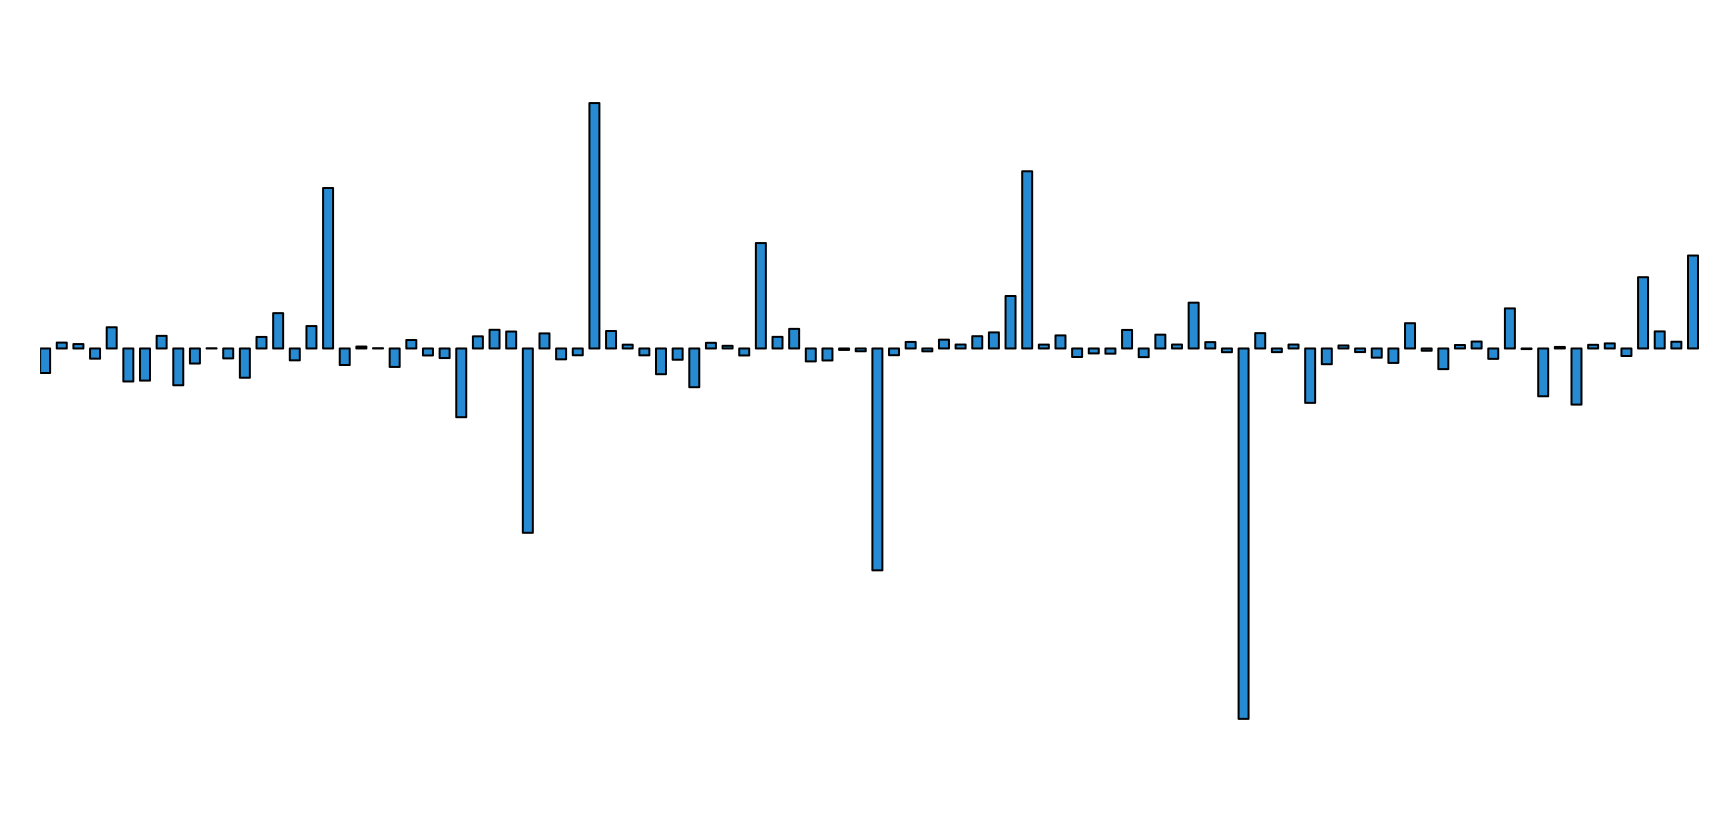
\includegraphics{LevyFlight/levy_length.pdf}
    \end{center}
    \caption{Distribution de 100 tirages aléatoire obéissant à une distribution de Lévy.
             \label{fig:levy_length}}
\end{figure}

\begin{figure}
    \begin{center}
        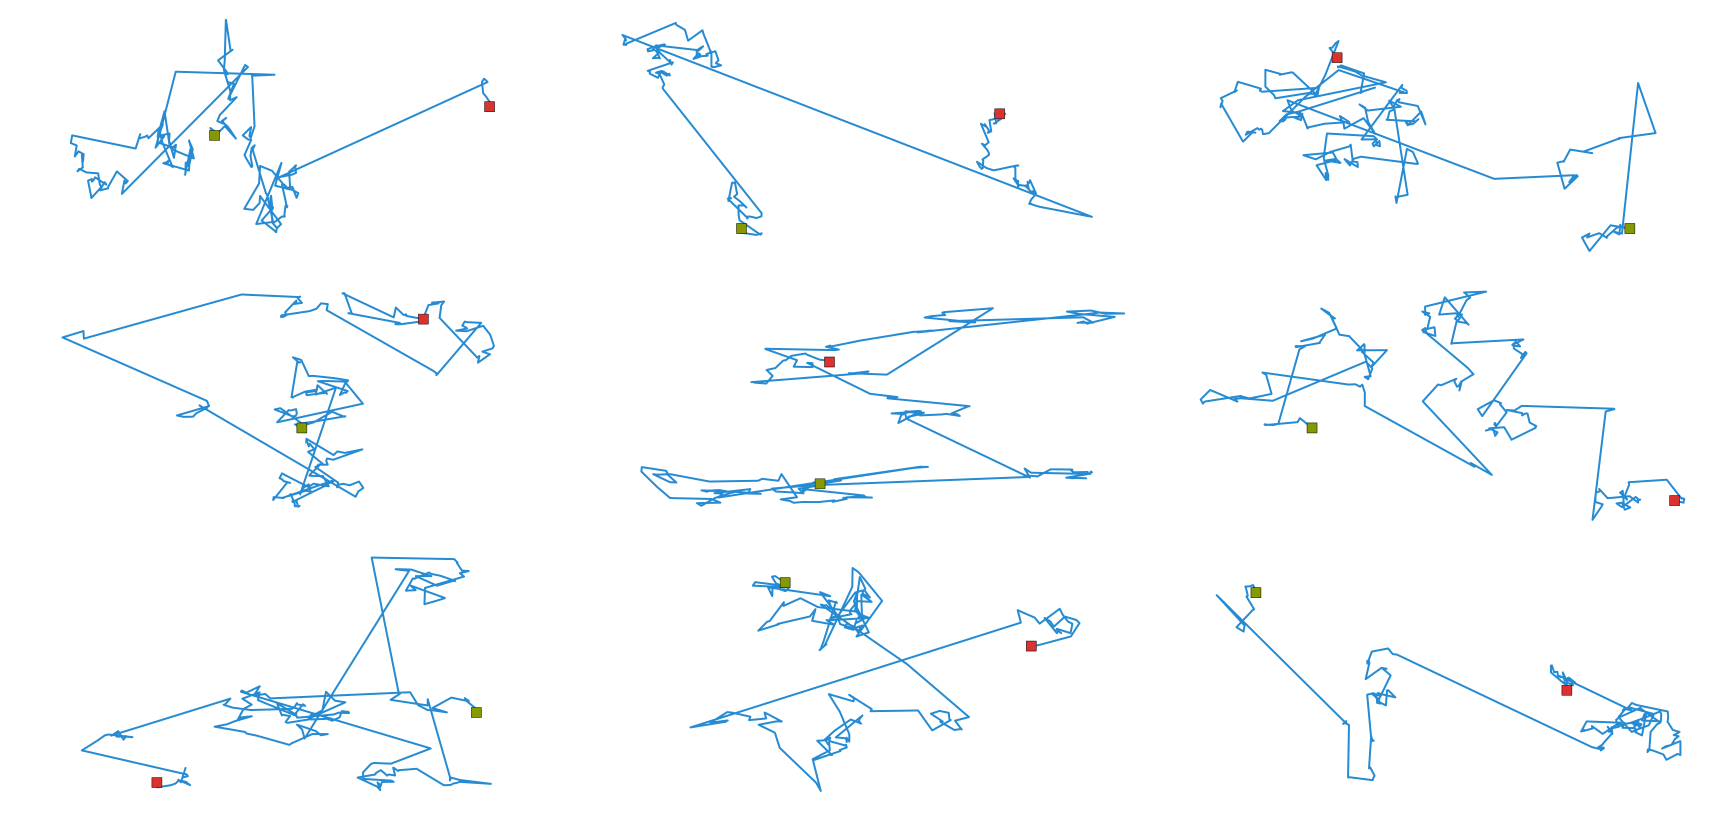
\includegraphics{LevyFlight/levy_flight.pdf}
    \end{center}
    \caption{Multiples vols de Lévy de 200 pas.
             \label{fig:levy_flight}}
\end{figure}

\begin{figure}
    \begin{center}
        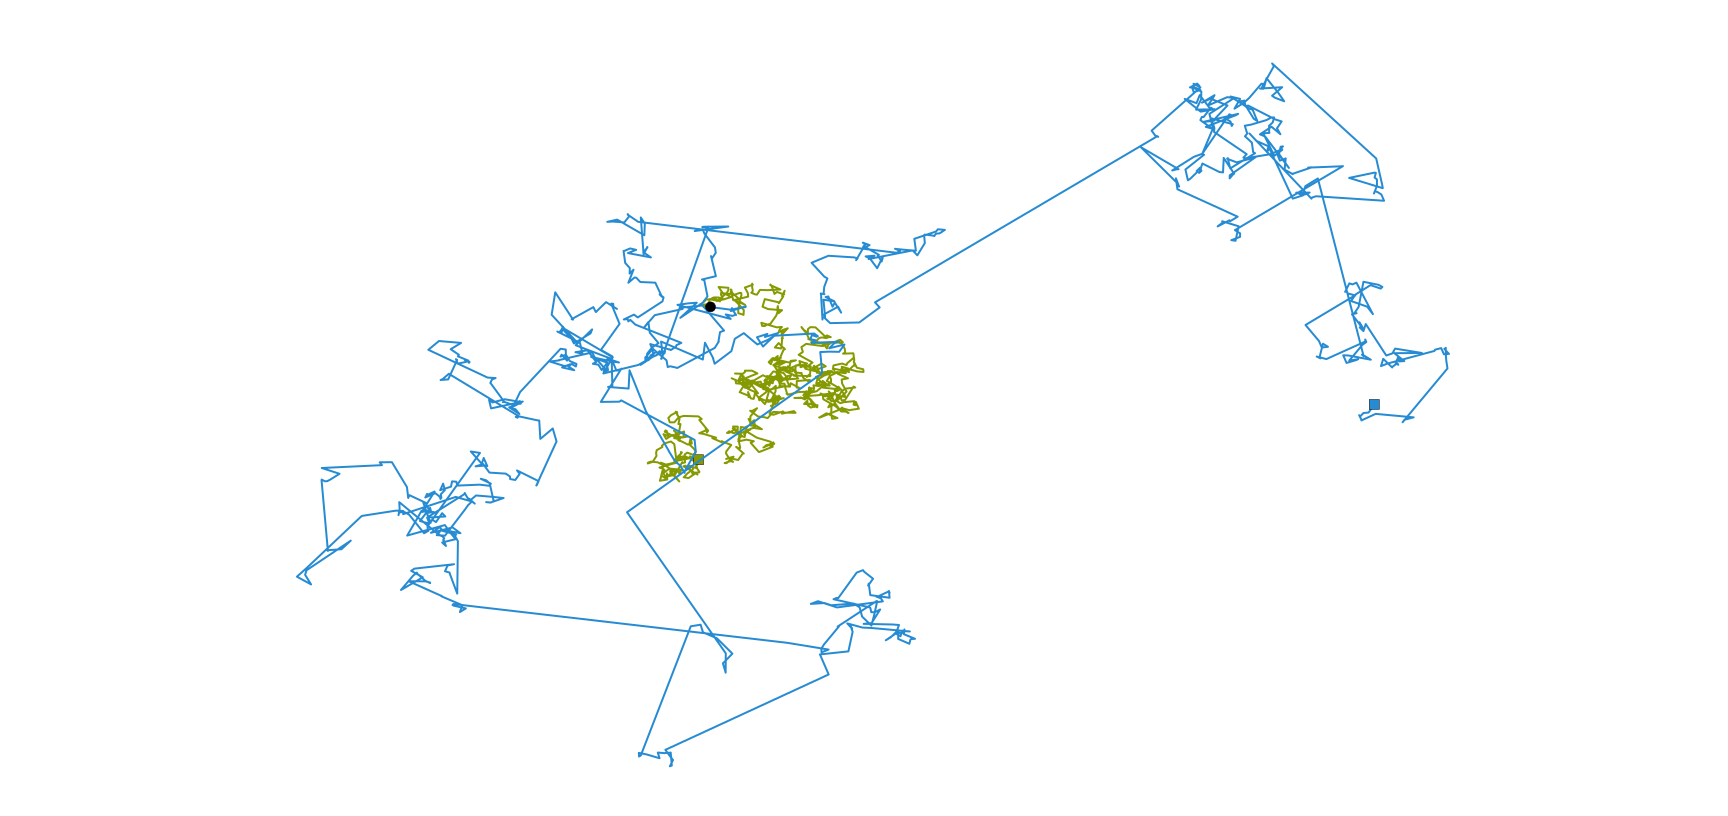
\includegraphics{LevyFlight/levy_vs_gaussian.pdf}
    \end{center}
    \caption{Mouvement browien (en vert) et vol de Lévy (en bleu) pour 200 pas aléatoires.
             \label{fig:levy_vs_gaussian}}
\end{figure}

\itodo{Ajouter des applications aux problèmes multi-objectifs}
Dans \cite{Sharma2012213}, vol de Lévy est employé pour améliorer l’algorithme ABC
pour faire une recherche locale autour de la meilleure solution actuelle. L’auteur
utilise un multiplicateur pour réduire la longueur des pas généré d’après \eqref{eq:step_len}.
De plus la meilleure solution actuelle est utilisée pour guider la recherche aléatoire et
peu être assimilé à un apprentissage. Le vol de Lévy a aussi été utilisé dans un algorithme
d’optimisation approchée, le Cuckko search. Cet algorithme est inspiré du comportement
parasitaire de la reproduction des cuculidés et a était adapté aux problèmes
multi-objectifs (\cite{Yang20131616}).
% subsubsection vol_de_lévy (end)

% - - - - - - - - - - - - - - - - - - - - - - - - - - - - - - - - - - - - - - -
\subsubsection{Apprentissage par opposition} % (fold)
\label{ssub:apprentissage_par_opposition}

La recherche par vecteur opposé (opposition-based learning) a été implémenté pour la première fois
en optimisation par \cite{Tizhoosh2005695,Rahnamayan2008155}. Il propose une méthode permettant de diversifier la
population sans connaissances à-priori.
% Opposite based learning method
\begin{Def}[OBLM~:~Opposition-Based Learning Method]\label{def:oblm}
La recherche par vecteur opposé (Opposition-Based Learning) permet de diversifier la
population sans connaissances à-priori.
Admettons un point de dimension $D$, $P(x_{1}, x_{2}, ..., x_{D})$ avec
$x_{1}, x_{2}, ..., x_{D}$ des valeurs bornées. Si $x_{i} \in [a_{i}, b_{i}]$ pour
$i = 1, 2, ..., D$ alors le point opposée est $\check{P}(\check{x_{1}}, \check{x_{2}}, ..., \check{x_{D}})$ suivant:
\[\check{x_{i}} = a_{i} + b_{i} - x_{i}\]
\end{Def}

Il est important de noter que les solutions sont comparées deux à deux par tournoi binaire, où
seule la meilleure solution entre l’initiale et son opposée est conservée. Admettons une solution
candidate $P(x_{1}, x_{2}, ..., x_{D})$ et son opposée $\check{P}(\check{x_{1}}, \check{x_{2}}, ..., \check{x_{D}})$,
alors si $f(\check{P}) \geq f(P)$ alors la solution $P$ est remplacé par $\check{P}$.
\ftodo{Illustration du tournoi binaire graphiquement}

Cette méthode a ensuite été améliorée (\cite{Rahnamayan2008155}) puis adaptée à
l’algorithme Differential evolution (DE). La méthode reprend la définition de base
mais définit plus clairement les limites et la portée de la méthode.
La méthode est utilisée durant la phase d’initialisation pour améliorer la diversité
en générant une population aléatoire de $n$ individus puis $n$ opposées.
Les solutions les plus performantes étant ensuite conservées pour obtenir une population
finale de $n$ individus.
Ensuite durant l’exécution de l’algorithme de nouvelles populations opposées sont générées.
Un coefficient $J_r$ est utilisé pour contrôler la probabilité de générer cette nouvelle
population opposée pour chaque itération.

La méthode a ensuite été testée sur un jeu de 15 fonctions de références (7 uni-modales
et 8 multi-modales). La nouvelle approche permet alors de trouver de meilleurs
résultats sur 14 des 15 fonctions. Il est aussi montré la supériorité de la
sélection par opposition par rapport au caractère aléatoire (\cite{Rahnamayan2008155,Rahnamayan2008906})
Il est aussi mis en avant que la probabilité de générer une population opposée
doit décroitre au fur et à mesure des itérations. En effet, la méthode permet de
réduire l’espace de recherche mais ralenti la convergence une fois cette intervalle
faible. Finalement il est proposé une intervalle de performance pour le coefficient si le problème
ne permet pas de déterminer un nombre fixe d’itération à-priori: $[0.1 < J_r < 0.4]$.

Cette approche a été appliquée avec succès dans le cas de l’algorithme ABC en couplage
avec un opérateur de mutation (\cite{Bi2011174}) ou encore en coopération avec une marche
aléatoire (\cite{Sharma2012213}).
Il a aussi été appliqué pour résoudre des problèmes plus complexe à objectifs multiples,
en combinaison avec un algorithme évolutionnaire (\cite{Ma201448}), ou encore avec le PSO (\cite{Gao2013114}).

Notre problème ne nous permettant pas d’avoir de connaissance à-priori, il nous est
impossible d’estimer le nombre d’itération nécessaires et l’utilisation d’un coefficient $J_r$
dynamique difficile.
% Au vu des recommandations et des applications déjà faites pour des problèmes mono-critères,
% ce coefficient sera fixé à 0.1 dans un premier temps.

\begin{figure}
    \begin{center}
        \includegraphics{abc/principe_obl.pdf}
    \end{center}
    \caption{Principe de fonctionnement de la recherche par vecteur opposée.
             \label{fig:OBL_method}}
\end{figure}
% subsubsection apprentissage_par_opposition (end)
% subsection ameliorer_l_exploration_et_l_exploitation (end)


% ------------------------------------------------------------------------------
\subsection{Prendre en compte les contraintes: quelle méthode ?} % (fold)
\label{sub:prendre_en_compte_les_contraintes_quelle_methode}
\itodo{Décrire les approches pour tacler les problèmes avec contraintes.
       Homorphous mapping, assimilation à un autre objectif (Voir Karaboga20113021)}

De nombreuses améliorations ont été proposées pour améliorer la vitesse de convergence
vers le ou les optimaux tout en évitant les optimums locaux. Cependant dans certaines
optimisation les objectifs sont dépendant de contraintes. Dans certaines conditions, il
est possible de résoudre ce problème de contrainte en bornant les variables à des solutions
réalisables mais ce n’est pas toujours possible. Lorsque ces contraintes ne peuvent pas être vérifiées
en amont de l’optimisation, il faut alors en tenir compte durant ce processus à l’aide
de méthode plus ou moins complexes.

La pénalité est l’approche la plus souvent retenue (\cite{EfrEnMezura-Montes2003}\munsure{Peut être mettre un vrai article ?}).
Cette approche demande la définition d’un facteur de pénalité qui doit être définie
avec précision pour pouvoir converger vers le/les solutions optimales qui respectent les
contraintes. Ce paramètre est dit: (i) statique si la pénalité est la somme pondérée des contraintes,
(ii) dynamique si le nombre d’itération influence le paramètre, (iii) adaptatif si l’information de la
recherche aide à sa détermination (\cite{Woldesenbet20073077}).
Enfin il est important de noter que une solution respectant toutes les contraintes sera toujours préférée
à une solution violant des contraintes même si l’évaluation des objectifs est meilleur. Il peut ainsi être
difficile d’atteindre certaines optimums\mtodo{Ceux qui sont entourés de violeur de contraintes} particulièrement
dans un espace de solutions faisables limitée.
\cite{Tsai201480} l’utilise avec deux essaims d’abeilles respectant respectivement l’algorithme
ABC et l’algorithme Bee Algorithm (BA) avec une population ajustée dynamiquement ou encore \cite{Karaboga20113021}
qui autorise des solutions ne respectant pas les contraintes à être ajoutées à la population. Ce dernier
utilise une facteur de pénalité déterminer dynamiquement évitant sa détermination empiriquement
(\cite{Deb2000311}\mtodo{Lire cet article !!}) comme les approches plus classiques de pénalité.
\\

\cite{EfrEnMezura-Montes2003} propose une méthode basée sur la sélection par tournoi binaire couplé à un mécanisme
déterministe permettant d’accepter des solutions infaisables. La probabilité de sélectionner une solution
seulement sur la performance des fonctions objectifs évolue est un paramètre adaptatif. Si durant une
certaine intervalle la déviation moyenne évolue faiblement alors la probabilité de pouvoir sélectionner
une solution uniquement sur optimalité des objectifs augmente et inversement.


\cite{Woldesenbet20073077} propose aussi une méthode ne demandant pas de paramètres supplémentaires
qui doivent être déterminé empiriquement. La première étape est de normalisé les objectifs et contraintes
grâce aux minimums et maximums à chaque itération. Ensuite une distance $d_{i}$ est
évaluée et la distance minimale est conservée. Soit $\tilde{f}$ respectivement la fonction objectif $i$ normalisée
et la somme des contraintes normalisées alors la distance s’écrit:
\begin{align}\label{eq:distance_measure}
    d_{i} = \begin{cases}
                v(x),                               \qquad & if\  r_{f} = 0\\
                \sqrt{\tilde{f}(x)^{2} + v(x)^{2}}, \qquad & otherwise\\
            \end{cases}
\end{align}
avec:
\begin{equation*}
    r_{f} = \frac{\text{Nbr de solutions faisable dans la population}}{\text{Taille de la population}}
\end{equation*}
Afin d’orienter la recherche vers un espace de solution faisables, une pénalité adaptative
est utilisé, $p_{i}(x)$, donnant un objectif final modifié de la forme: $F_{i}(x) = d_{i}(x) + p_{i}(x)$.
La population peut ainsi accepter des solutions ne respectant pas les contraintes mais
l’archive (optimisation multi-objectifs) elle n’accepte que des solutions faisables.
% subsection prendre_en_compte_les_contraintes_quelle_methode (end)


% ------------------------------------------------------------------------------
\subsection{Vers un outil d’aide à la décision par optimisation multi-objectif} % (fold)
\label{sub:vers_un_outil_d_aide_à_la_décision_par_optimisation_multi_objectif}
\itodo{Ajouter une vision globale du processus d’optimisation sous forme de graphique
      servant de résumé du chapitre.}

L’algorithme ABC modifié (Fig.~\ref{fig:abc_modifie}) comprend les même phases que l’original. La différence réside
dans le déroulement de ces phases. En effet plusieurs technique présentées ci-avant
ont été implémentées afin d’améliorer l’exploitation et l’exploration de l’algorithme.
Enfin une archive par $\epsilon$-dominance est utilisé pour maintenir les solutions
non-dominées formant le front de Pareto. Cette archive est mise à jour après chaque
évaluation contrairement aux sources qui ne sont mis à jour que après chaque phase.

\begin{figure}
    \begin{center}
        \includegraphics[width=10cm, height=15cm]{abc/algorithme_complet.png}
    \end{center}
    \caption{Description globale de l’algorithme ABC modifié. Chaque phase renvois à un algorithme.
             \label{fig:abc_modifie}}
\end{figure}

Dans un premier temps l’algorithme initialise l’archive grâce aux objectifs et aux valeurs
d’epsilons puis la population est initialisé aléatoirement par OBL afin d’obtenir une meilleure diversité
(Algorithm~\ref{alg:init_phase}). Ensuite on entre dans le processus itératif
tant que la ou les conditions d’arrêts ne sont pas atteintes. Les différentes phases
sont les suivantes: (i) Phase des butineuses (Algorithm~\ref{alg:employed_phase}) qui explore l’espace de décision avec des vols de
Lévy, (ii) Phase des ouvrières (Algorithm~\ref{alg:onlooker_phase}) qui utilisent les informations acquises par les butineuses
et améliorent les sources choisies \eqref{eq:attribution_prob_to_source}, (iii) Phase des éclaireuses
(Algorithm~\ref{alg:scout_phase}) qui réinitialisent une source si elle est non fructueuse.
La longueur du vol de Lévy est définie par:
\begin{equation}\label{eq:levy_flight}
  LevyFlight = scaleFactor \times stepLength \times RandUniform(0, 1)
\end{equation}
avec $stepLength$ définie par \eqref{eq:step_len} et $scaleFactor$ fixé à 0.01.\\


% Attribution des probabilités
La probabilité de choisir une source $k$ par une ouvrière est elle définie comme:
\begin{subequations}\label{eq:attribution_prob_to_source}
  \begin{align}
    prob_{k} = &\frac{Qualite(\vec{x}_{k})}{\sum_{i=1}^{NbrSources} Qualite(\vec{x}_{i})} \\[1em]
    Qualite(\vec{x}_{k}) = &\frac{Dominance(k)}{NbrSources}
  \end{align}
  avec \emph{Dominance(k)} le nombre de source que la source $k$ domine, et \emph{Fitness}
  la qualité de la source en tenant comptes des contraintes comme définies en.
\end{subequations}

% Phase d’initialisation
\begin{algorithm}\label{alg:init_phase}
  \SetAlgoVlined
  \emph{Initialisation des sources sur l’ensemble de l’espace de décision}\;
  \For{$i \leftarrow 0$ \KwTo \ANbrSources}
  {
    \emph{Initialisation des critères pour chaque source}\;
    \For{$j \leftarrow 0$ \KwTo \ANbrCriteria}
    {
      \AComment{Génération aléatoire de la position initiale}
      $x_{ij} = x_{j}^{min} + RandUniform(0, 1) \times (x_{j}^{max} - x_{j}^{min})$\;
      avec $RandUniform$ un tirage aléatoire suivant une loi uniforme, et $x_{j}^{min}$, $x_{j}^{max}$
      respectivement le minimum et le maximum du critère $j$\;
      \vspace{1em}  % Add some space between two blocs
      \AComment{Génération de la position opposée suivant Definition~\ref{def:oblm}}
      $ \check{x_{ij}} = a_{j} + b_{j} - x_{ij}$\;
      avec $a_{j}$, $b_{j}$ respectivement les bornes inférieures et supérieurs du critère
    }
    \If{$\ASource_{i}$ respecte toutes les contraintes}
    {
      \AComment{On ajoute la source initial à l’archive}
      $\AArchive \pluseq \ASource_{i}$\;
    }
    \If{$\check{\ASource_{i}}$ respecte toutes les contraintes}
    {
      \AComment{On ajoute la source opposée à l’archive}
      $\AArchive \pluseq \check{\ASource_{i}}$\;
    }
  }
  \AComment{On ne conserve que une seule position par source}
  Mise à jour de la position des \ASources d’après Algorithm~\ref{alg:maj_phase}\;
  \caption{Initialisation des sources par OBLM (Opposite-Based Learning Method).}
\end{algorithm}

% Maj des sources
\begin{algorithm}\label{alg:maj_phase}
  \SetAlgoVlined
  Récupérer le maximum et minimum pour chaque objectif\;
  Récupérer le maximum pour chaque contrainte\;
  \For{$i \leftarrow 0$ \KwTo \ANbrSources}
  {
    Normaliser les objectifs et les contraintes avec ()\;
    Calculer la valeur de distance $\vec{d_{i}}$ en utilisant \eqref{eq:distance_measure}\;
    Calculer la pénalité $\vec{p_{i}}$ d’après ()\;
    \AComment{Attribuer les nouvelles valeurs d’objectifs aux sources}
    $\vec{F_{i}} = \vec{d_{i}} + \vec{p_{i}}$\;
    \If{$\check{\vec{F_{i}}} \succ \vec{F_{i}}$}
    {
      \AComment{On remplace la position de la source par la nouvelle}
      $\vec{x_{i}} \leftarrow \check{\vec{x_{i}}}$\;
      \AComment{On réinitialise le nombre d’échec pour la source $i$}
      $\ATrial_{i} \leftarrow 0$\;
    }
    \Else
    {
      \AComment{On incrémente le nombre d’échec pour la source $i$}
      $\ATrial_{i} \pluseq 1$\;
    }
    avec $\vec{F_{i}}$, $\check{\vec{F_{i}}}$ respectivement les vecteurs objectifs
    normalisés pour l’ancienne et la nouvelle position.\;
  }
  \caption{Mise à jour des sources}
\end{algorithm}

% Phase des butineuses
\begin{algorithm}\label{alg:employed_phase}
  \SetAlgoVlined
  \AComment{Exploration des sources par les \AEmployed}
  \For{$i \leftarrow 0$ \KwTo \ANbrSources}
  {
    Sélection aléatoire d’une source $k$ dans l’\AArchive\;
    \AComment{Génération d’une nouvelle position pour la \ASource $i$}
    \For{$j \leftarrow 0$ \KwTo \ANbrCriteria}
    {
      \begin{algomathdisplay}
        \check{x_{ij}} =%
          \begin{cases}
            x_{ij} + \ALevyFlight_{ij} \times (x_{ij} - x_{kj}) &\ \ATirage < \AMR \\
            x_{ij}                                      &\ sinon
          \end{cases}
      \end{algomathdisplay}
      avec \ATirage un nombre aléatoire uniforme (entre 0 et 1),
      \AMR un paramètre contrôlant le nombre de modifications
      et \ALevyFlight définie par \eqref{eq:levy_flight}\;
    }
    \If{aucun critère n’a été modifié}
      {
        \AComment{Sélection aléatoire d’un critère $j$ à mettre à jour}
        $\check{x_{ij}} = x_{ij} + \ALevyFlight_{ij} \times (x_{ij} - x_{kj})$\;
      }
    \If{$\ASource_{i}$ respecte toutes les contraintes}
    {
      \AComment{On ajoute la source initial à l’archive}
      $\AArchive \pluseq \ASource_{i}$\;
    }
    \If{$\check{\ASource_{i}}$ respecte toutes les contraintes}
    {
      \AComment{On ajoute la source opposée à l’archive}
      $\AArchive \pluseq \check{\ASource_{i}}$\;
    }
  }
  \AComment{On ne conserve que une seule position par source}
  Mise à jour de la position des \ASources d’après Algorithm~\ref{alg:maj_phase}\;
  \caption{Phase des butineuses.}
\end{algorithm}

% Phase des ouvrières
\begin{algorithm}\label{alg:onlooker_phase}
  \SetAlgoVlined
  \AComment{Exploitation des sources par les \AOnlookers}
  \For{$\ABee \in \AOnlookers$}
    {
      Sélection aléatoire d’une \ASource $i$ selon la probabilité
      définie par l’équation \eqref{eq:attribution_prob_to_source} (Sélection par roulette)\;
      Génération d’une nouvelle position pour la \ASource $i$ selon Algorithm~\ref{alg:employed_phase}
      (lignes 3 à 16)\;
    }
  \AComment{On ne conserve que une seule position par source}
  \AComment{Plusieurs \AOnlookers peuvent modifier la même source}
  Mise à jour de la position des \ASources qui ont été modifiées d’après Algorithm~\ref{alg:maj_phase}\;
  \caption{Phase des ouvrières.}
\end{algorithm}

% Phase des éclaireuses
\begin{algorithm}\label{alg:scout_phase}
  \SetAlgoVlined
  \For{$i \leftarrow 0$ \KwTo \ANbrSources}
  {
    \If{$\ATrial_{i} > \AMaxTrial$ }
    {
      \AComment{Exploration par les \AScouts}
      Génération de deux nouvelles positions suivant Algorithm~\ref{alg:init_phase}
      (lignes 4 à 16)\;
    }
  }
  \AComment{On conserve la meilleure solution parmi les deux nouvelles}
  Mise à jour de la position des \ASources d’après Algorithm~\ref{alg:maj_phase}\;
  \caption{Phase des éclaireuses.}
\end{algorithm}
% subsection vers_un_outil_d_aide_à_la_décision_par_optimisation_multi_objectif (end)
% section construction_d_un_outil_d_aide_à_la_decision (end)


\chapter{Optimisation multi-objectifs d’un \abr{SSC} couplé à une \abr{MEPOS}}
%!TEX root = ../main.tex
% Chapitres/Chap4-OptimisationSystemeSolaire.tex

\iunsure{Description commune de Bordeaux et Strasbourg pour éviter répétition (section 2, 3)}
\iunsure{Relancer les simulations Pareto optimales avec Dymola pour comparaison}

% Pour optimisation
% Par exemple un pas de \num{0.1} avec des bornes min de \num{0} et max de \num{0.5} donnera
% les variations possibles suivantes~: (\num{0} - \num{0.1} - \num{0.2} - \num{0.3} - \num{0.4} - \num{0.5}).



% ..............................................................................
% ..............................................................................
\section{Description de l’étude de cas} % (fold)
\label{sec:description_de_l_etude_de_cas}
% ------------------------------------------------------------------------------
\subsection{Scénarios} % (fold)
\label{sub:scenarios}
L’étude de cas est réalisée sur le bâtiment utilisée pour l’étude paramétrique.
Les scénarios pour les charges internes (équipements, éclairage, et occupants) sont
issues de la simulation de référence (\ref{sub:scenarios_de_reference}). De même
le scénario de référence est retenue pour la consigne de chauffage ($19$-$18$-$16$)
et le scénario de ventilation ($90-20$).
Pour le puisage en $ECS$, le profil $Réaliste$ est retenue avec la prise en compte des
variations hebdomadaires et mensuelles (\ref{ssub:puisage_en_eau_chaude_sanitaire}).
En effet, comme il a été montré, il est important de tenir compte de la variation
du profil de puisage au cours de l’année afin de ne pas sur-estimer la performance
du $SSC$.
% subsection scenarios (end)



% ------------------------------------------------------------------------------
\subsection{Paramètres a priori} % (fold)
\label{sub:parametres_a_priori}
~
\iunsure{Ajouter explication variables discrètes}
\ifix{Vérifier valeurs bornes sensibilité}
\ifix{Vérifier capteurs utilisés dans l’otpimisation}
\itodo{Ajouter différence Strasbourg et Bordeaux}


Comme décrit dans le chapitre précédent, une analyse de sensibilité est nécessaire
afin de réduire la cardinalité du problème, évitant ainsi de simuler des variations
non influentes relativement aux autres paramètres.
L’étude de cas est réalisée pour deux climat différents, Bordeaux et Strasbourg,
et un ensemble de \num{22} paramètres a priori est retenue (\tabref{tab:facteur_sensibilite})
en faisant varier à la fois la performance de l’enveloppe et les caractéristiques du $SSC$.
\itodo{Vérifier sources}
Au niveau des isolants, les bornes inférieures et supérieures représentent respectivement
le niveau recommandé pour la \textit{RT\,2005} et le niveau \textit{MEPOS}.
La plage de variation pour les surfaces vitrées a été fixée arbitrairement à plus ou moins \SI{20}{\percent}
de leur valeur d’origine. L’étude ne cherche pas à évaluer l’impact de l’inclinaison
des capteurs qui est imposée par la géométrie du bâtiment, elle est donc fixée à
\SI{33}{\percent} soit \SI{18.9}{\degree}.


% - - - - - - - - - - - - - - - - - - - - - - - - - - - - - - - - - - - - - - -
\subsubsection{Production d’électricité} % (fold)
\label{ssub:production_d_electricite}
L’étude de cas cherchant à obtenir un bâtiment ayant une consommation très faible, il est
nécessaire d’introduire une production locale d’électricité. Cette production permettra de
couvrir l’énergie consommée par les équipements internes (électroménager et éclairage)
ainsi que la $Conso_{app}$.

La même variation de surface est considérée pour les capteurs $PV$ et thermiques~:
\SI{\approx 7}{\metre\squared}. En effet, seul la production de $PV$ peut
compenser les consommations de charges internes et il est plus intéressant d’évaluer son
influence par rapport à une surface équivalent en solaire thermique. De plus la surface
minimale de $PV$ a été définie afin de couvrir \SI{75}{\percent} (\SI{\approx 2330}{\kWh})
de la consommation des équipements internes (\SI{\approx 3082}{\kWh}).

Afin de d’évaluer correctement la production solaire, la surface disponible en toiture
doit être cependant être correctement partagée. Comme il a été vu au chapitre 2, la
$Prod_{sol}$ dépend fortement de l’orientation des capteurs solaires thermiques. Ils sont
donc prioritaire sur le pan Sud. De plus, il est aussi nécessaire de tenir compte de la
géométrie à la fois de la toiture et des capteurs. La maison comporte une toiture quatre
pans, chaque pan est donc triangulaire, et les capteurs eux sont de forme rectangulaire.
Il apparaît donc clairement que l’approche naïve qui consiste à considérer la surface
totale de la toiture comme disponible n’est pas valable~: seule une partie est réellement
utilisable. Un algorithme de \enquote{packaging} a donc été développé afin d’évaluer le
nombre de capteurs pouvant loger sur chaque pan de toiture et le détail du calcul est
disponible en annexe (\ref{cha:repartition_des_capteurs}).

Finalement, contrairement au $SSC$ qui est évalué uniquement \emph{sur une période
s’étendant du $1^{er}$ octobre au $30$ avril}, la production $PV$ doit être évalué sur
l’année complète. Pour rappel, la période de simulation est limitée à la période de
l’année où le $SSC$ n’est pas complètement indépendant pour les combinaisons de paramètres
les plus défavorables (\ref{par:periode_de_simulation}). Ainsi sur le reste de l’année la
$Conso_{app}$ est équivalente à la $Conso_{pompes}$ qui est négligeable au regard des
résultats de l’analyse paramétrique. L’ensemble des combinaisons existantes entre $PV$ et
capteurs thermiques est donc simulée sur l’année en amont.
% subsubsection production_d_electricite (end)


% - - - - - - - - - - - - - - - - - - - - - - - - - - - - - - - - - - - - - - -
\subsubsection{Variables qualitatives} % (fold)
\label{ssub:variables_qualitatives}
La méthode de Morris nécessite que l’ensemble des variables soient quantitatives et chaque
paramètre varie indépendamment. Il n’est donc pas possible d’évaluer directement
l’influence des capteurs solaires ou des vitrages qui sont des variables qualitatives.

Afin de tenir compte de ces paramètres, leurs caractéristiques principales sont considérés
comme des paramètres indépendants. Dans le cas des capteurs solaires, le rendement optique
$\eta_{0}$ et les coefficients $a_{1}$ et $a_{2}$ sont retenues. Dans le cas des vitrages
les caractéristiques principales souvent utilisées sont le $U_{g}$ et le $g$ permettant
respectivement d’évaluer la résistance au transfert thermique et au passage de l’énergie
solaire. Les vitrages étant définies de manière détaillé, les paramètres $Émis_{ext}$
et $\tau_{sol}$ sont retenues. Bien que la méthode de Morris permettent de
regrouper un jeu de paramètre en un paramètre unique (groupe), les paramètres restent
indépendants et l’approche n’est donc pas retenue. Ainsi les combinaisons réalisées
représentent des capteurs / vitrages hypothétiques dont la faisabilité technique n’est pas
garantie. L’approche permet cependant de mettre en exergue l’importance relative de chaque
caractéristique sur la performance du capteur ou du vitrage et son impact global au niveau
du $SSC$. De plus, les autres paramètres définies a priori peuvent tenir compte de la
forte variabilité des capteurs et des vitrages. En effet, il est possible qu’il existe des
interactions entre les vitrages ou capteurs solaires et les autres facteurs quantitatifs.
% subsubsection variables_qualitatives (end)

\begin{table}
\centering
\caption{Liste des paramètres a priori utilisés pour l’analyse de sensibilité.}
\label{tab:facteur_sensibilite}
\begin{tabular}{l c c l}
  \toprule
  \addlinespace
                                               & Borne min     & Borne max   & Remarques                                                            \\
  \addlinespace
  \multicolumn{4}{l}{\bm{$SSC$}}                                                                           \\
  \midrule
  Nombre capteurs                              & \num{2}       & \num{5}     & \num{4.64} -- \SI{11.6}{\metre\squared}                              \\
  $\eta_{0}$                                   & \num{0.63}    & \num{0.84}  & \multirow{3}{*}{Diversité issue de \href{www.solar-rating.org}{ICC-SRCC}}   \\
  $a_{1}$                                      & \num{0.65}    & \num{6.7}   &                                                                      \\
  $a_{2}$                                      & \num{0.00069} & \num{0.29}  &                                                                      \\
  $Ech_{sol}^{pos}$                            & \num{0.8}     & \num{1.3}   & Position relative à la taille du ballon                              \\
  Volume ballon tampon                         & \num{100}     & \num{500}   & \multirow{2}{*}{Dimensions adaptées proportionnellement}             \\
  Volume ballon $ECS$                          & \num{100}     & \num{500}   &                                                                      \\
  $R$ ballon sanitaire                         & \num{7}       & \num{10}    & \multirow{2}{*}{Variation uniquement de l’épaisseur de l’isolant}    \\
  $R$ ballon tampon                            & \num{7}       & \num{10}    &                                                                      \\
  $Isolant_{réseau}^{épaisseur}$               & \num{0.013}   & \num{0.04}  & Résistance dépendant du nombre de capteurs                           \\
  Consigne solaire                             & \num{18}      & \num{24}    &  -                                                                   \\
  $DeltaT_{sol}$                               & \num{5}       & \num{15}    &  -                                                                   \\
  \\
  \addlinespace[\defaultaddspace]
  \multicolumn{4}{l}{\textbf{Enveloppe du bâtiment}}                                                                              \\
  \midrule
  $R$ plancher                                 & \num{6}       & \num{10}    &  -                                                                   \\
  $R$ murs                                     & \num{4}       & \num{7}     &  -                                                                   \\
  $R$ plafond                                  & \num{6}       & \num{10}    &  -                                                                   \\
  $\tau_{sol}$                                 & \num{0.643}   & \num{0.849} & \multirow{2}{*}{Variation des vitrages Nord et Ouest uniquement}     \\
  $Émis_{ext}$                                 & \num{0.037}   & \num{0.837} &                                                                      \\
  Surface vitrée Est                           & \num{4.3}     & \num{6.46}  & \multirow{4}{*}{Surface totale \SI{26.4}{\metre\squared}}            \\
  Surface vitrée Nord                          & \num{0.46}    & \num{0.684} &                                                                      \\
  Surface vitrée Sud                           & \num{5.42}    & \num{8.13}  &                                                                      \\
  Surface vitrée Ouest                         & \num{2.3}     & \num{3.89}  &                                                                      \\
  \\
  \addlinespace[\defaultaddspace]
  \multicolumn{4}{l}{\textbf{Production d’électricité}}                                                                     \\
  \midrule
  Surface $PV$                                 & \num{12}       &  \num{19}   &  Capteurs thermiques prioritaires sur le pan Sud                                                             \\
  \bottomrule
  \end{tabular}
\end{table}
% subsection parametres_a_priori (end)



% ------------------------------------------------------------------------------
\subsection{Objectifs et contraintes} % (fold)
\label{sub:objectifs_et_contraintes}
% - - - - - - - - - - - - - - - - - - - - - - - - - - - - - - - - - - - - - - -
\subsubsection{Approche naïve} % (fold)
\label{ssub:approche_naive}
Fort de l’expérience acquise à travers l’étude paramétrique, les objectifs sont formalisés
de la manière suivante~:
\begin{itemize}
  \item Augmenter le $F_{sol}^{ECS}$
  \item Augmenter le $F_{sol}^{CH}$
  \item Réduire la $Conso_{app}$
\end{itemize}
De plus une contrainte est introduite afin de vérifier que le bâtiment final
est un bâtiment passif~: $|Conso_{totale}| \leq \SI{300}{kWh}$ \eqref{eq:conso_totale}.
De cette manière, les bâtiments produisant localement respectivement trop ou pas assez d’énergie sont
écartés. De plus cette restriction permet de guider la recherche vers un le front de
Pareto.

\begin{equation} \label{eq:conso_totale}
  Conso_{totale} = Conso_{app} + Conso_{équipements} + Conso_{éclairage} - Prod_{PV}
\end{equation}

Cependant formulé de cette manière, l’approche comporte plusieurs failles. Premièrement,
il est clair que même si les \num{3} objectifs ne sont pas impactés par les mêmes
paramètres, une tendance commune est identifiable. Ainsi, sans objectifs évoluant de
manière \enquote{contradictoires} l’optimisation risque de converger vers un ensemble
de solution très réduites voir une solution unique.

Deuxièmement, l’approche introduit un biais important sur la surface de $PV$. Afin de
respecter la contrainte, deux configurations extrêmes sont possibles~:
\begin{itemize}
  \item Avoir beaucoup de $PV$ et peu de capteurs thermiques
  \item Avoir beaucoup de capteurs thermiques et suffisamment de $PV$ pour couvrir
        les consommations des équipements internes.
\end{itemize}
Cependant, une fois que la surface de $PV$ permettant d’obtenir une $Conso_{totale}$
a atteinte la limite basse imposée par la contrainte (\SI{300}{kWh}), elle ne peut plus
augmenter car la contrainte serait violée (production trop importante d’électricité). De plus,
augmenter la surface de $PV$ impacte aucun des objectifs, les solutions avec une surface
de $PV$ plus importante seront toujours rejetées.

Afin que la surface de $PV$ soit influente sur au moins un objectif il est possible
de minimiser la $Conso_{totale}$ au lieu de minimiser la $Conso_{app}$.
Cependant, il a été vu au chapitre précédent que la dominance de Pareto implique que une solution
est meilleure qu’une autre si et seulement si elle est meilleure sur un objectif et au moins
aussi bonne sur les autres (\defref{def:dominance_de_pareto}). Il est donc clair que
cette modification ne permet pas de corriger ce biais qui réduit fortement l’espace
de décision comme celui des solutions.
% subsubsection approche_naive (end)


% - - - - - - - - - - - - - - - - - - - - - - - - - - - - - - - - - - - - - - -
\subsubsection{Approche retenue} % (fold)
\label{ssub:approche_retenue}
Afin de palier aux difficultés rencontrées, une autre formulation est proposée où les objectifs
sont~:
\begin{itemize}
  \item Augmenter le $F_{sol}^{ECS}$
  \item Augmenter le $F_{sol}^{CH}$
  \item Réduire la $Prod_{PV}$
\end{itemize}
De plus la contrainte est exprimée comme~: $|Conso_{totale}| \leq 300$

Dans cette nouvelle formulation, l’ensemble des paramètres influence au minimum un des
objectifs. Il est aussi clair que les deux premiers objectifs sont en contradiction nette
avec le dernier et le biais n’existe donc plus. En effet, il est maintenant possible en
théorie d’obtenir des solutions avec une surface de $PV$ importante et une surface de
capteur thermique faible et inversement.
Le problème est maintenant correctement formulé pour explorer l’espace de décision et
répondre au problème initial~: réaliser une maison passive dont les besoins sont couverts
par l’énergie solaire.
% subsubsection approche_retenue (end)
% subsection objectifs_et_contraintes (end)
% section description_de_l_etude_de_cas (end)





% ..............................................................................
% ..............................................................................
\section{Vers un modèle simplifié} % (fold)
\label{sec:vers_un_modele_simplifie}
% ------------------------------------------------------------------------------
\subsection{Réduction de la cardinalité} % (fold)
\label{sub:reduction_de_la_cardinalite}
~
\itodo{Décrire les résultats obtenues Bordeaux et Strasbourg}
\iunsure{Faire en même temps ou faire des sections}

L’analyse de Morris a été réalisée en considérant \num{15} trajectoires uniques à travers
\num{4} niveaux. Les résultats sont analysés sur les indicateurs caractéristiques d’un $SSC$
(le $F_{sol}^{CH}$, le $F_{sol}^{ECS}$, et la $Conso_{app}$) mais aussi sur les parts
actives et passives du chauffage solaire, respectivement notées $Prod_{sol}^{active}$ et
$Prod_{sol}^{passive}$. En effet, les ballons étant dans le bâtiment, une partie de
l’énergie solaire est fournie par leurs déperditions.

\itodo{Faire en détail la description avec des chiffres pour moyenne et écart type}
\itodo{$Conso_{app}$}
Les résultats (\figref{fig:morris_analysis_indicateurs}) sur la $Conso_{app}$ montrent
que les paramètres $a_{1}$, $a_{2}$, $\eta_{0}$, $Émis_{ext}$, le volume du ballon $ECS$,
la surface vitrée à l’Est et au Sud, la résistance thermique des murs et du plafond, ainsi que le nombre de capteurs thermiques,
sont tous influents. L’ensemble des paramètres influents on un impact linéaire à l’exception
du volume du ballon $ECS$ dont l’influence est ou non-linéaire ou avec des interactions.
Il apparaît aussi que le niveau d’isolation des ballons comme des canalisations ne soit pas
très impactant.

Ainsi au regard de ces premiers résultats le performance thermique des vitrage doit être
considéré tout comme le type de capteur solaire utilisé car ces trois indicateurs caractéristiques
sont influents.

\itodo{$F_{sol}^{ECS}$}
Sur l’indicateur $F_{sol}^{ECS}$ les facteurs ayant une influence linéaire sont
peu nombreux~: la surface de capteur et ces caractéristiques ($a_{1}$, $a_{2}$, $\eta_{0}$)
ainsi que le volume du ballon sanitaire. La $Ech_{sol}^{pos}$ quand à elle a une influence
non-linéaire ou avec des interactions.


\itodo{$F_{sol}^{CH}$}
Sur l’indicateur $F_{sol}^{CH}$ les facteurs ayant une influence linéaire sont~: la
surface des capteurs thermiques, le volume des deux ballons, les \num{3} coefficients
caractéristiques des capteurs solaires ($a_{1}$, $a_{2}$, et $\eta_{0}$), la performance
des vitrages ($Émis_{ext}$), la résistance thermique des murs et du plafond, ainsi que le
$DeltaT_{sol}$. Le coefficient $a_{1}$ est important car il a un $\sigma$ et un $\mu^{*}$
moyens alors que les autres sont caractérisés par un $\mu^{*}$ important mais un $\sigma$
faible. Le volume du ballon sanitaire et le $DeltaT_{sol}$ ont quand à eux une influence
non linéaire ou avec des interactions.
Il est aussi observé que les paramètres n’influence pas de la même manière le $F_{sol}^{CH}$.
Certains paramètres comme la performance thermique des mur, du plancher et de la consigne solaire
influencent uniquement la $Prod_{sol}^{active}$ alors que
d’autres comme la résistance thermique des ballons influence uniquement la $Prod_{sol}^{passive}$.
Il peut aussi être noté que le volume du ballon tampon influence plus fortement la
$Prod_{sol}^{passive}$ alors que l’on observe l’inverse pour la performance thermique
des vitrages.


\itodo{$Conso_{totale}$}
Si on s’intéresse à l’indicateur de $Bilan_{pos}$ ($\nicefrac{Prod_{PV}}{Conso_{totale}}$)
il est observé une très forte influence linéaire de la surface de $PV$. Les autres paramètres
ayant une influence modéré~: surface des capteurs, isolation des vitrages, $a_{1}$, $\eta_{0}$
et le ballon sanitaire qui encore une fois a un impact non-linéaire ou avec des interactions.
En effet, la surface de $PV$ est le seul facteur permettant de couvrir les consommations
électriques des équipements internes qui représente la majorité des consommations. Il est donc
évident que ce paramètre est fortement influent.


Au regard de cette analyse il apparaît important de considérer les caractéristiques des capteurs et
des vitrages. Ainsi, pour l’optimisation un jeu de capteurs solaires et de vitrages représentatifs
des variations étudiées est retenu (\tabref{tab:capteurs_specs}, \tabref{tab:carac_vitrages}).
L’ensemble des paramètres conservés est récapitulé dans la \figref{fig:graphe_influence} où il
apparaît que les variations retenus sont à la fois sur l’enveloppe et le système.
\itodo{Expliquer que c’est intéressant donc de les étudier ensembles}
Il existe ainsi des compromis intéressants entre la qualité de l’enveloppe, la surface de $PV$, et
les caractéristiques du $SSC$. De plus cette méthode de criblage a permise de passer de
\num{19} paramètres à \num{12} réduisant ainsi fortement la cardinalité du problème.




\begin{figure}
    \begin{center}
        \ftodo{$\sigma$ et $\mu^{*}$ colonne Bordeaux et Strasbourg}
        % \includegraphics{Ressources/Images/Modelisation/air_modes.pdf}
    \end{center}
    \caption{Résultat de l’analyse de Morris pour différent indicateurs.
             \label{fig:morris_analysis_indicateurs}}
\end{figure}


\begin{landscape}
    \begin{figure}
      \begin{center}
          \ftodo{Ajouter le graphe d’influence complet}
          \includegraphics{Ressources/Images/Sensibilite/graphInfluence.pdf}
      \end{center}
      \caption{Résultat de l’analyse de Morris pour différent indicateurs.
               \label{fig:graphe_influence}}
  \end{figure}
\end{landscape}

\begin{table}
\centering
\caption{Liste des paramètres retenus pour l’optimisation.}
\label{tab:facteur_retenues}
\begin{tabular}{l c c c c l}
  \toprule
  \addlinespace
                       & Min        & Max         & Catégorie  & Pas        & Remarques                                \\
  \addlinespace
  \multicolumn{5}{l}{\bm{$SSC$}}         \\
  \midrule
  Nombre capteurs      & \num{2}    & \num{5}     & Discrète    & \num{1}    & \num{4.64} -- \SI{11.6}{\metre\squared}   \\
  Type de capteur      & -          &  -          & Qualitative & -          & Voir \tabref{tab:capteurs_specs}   \\
  $Ech_{sol}^{pos}$    & \num{0.8}  &  \num{1.3}  & Continue    & -          & Position relative à la taille du ballon     \\
  Volume ballon tampon & \num{100}  &  \num{500}  & Discrète    & \num{50}   & \multirow{2}{*}{Dimensions adaptées proportionnellement}   \\
  Volume ballon $ECS$  & \num{100}  &  \num{500}  & Discrète    & \num{50}   &    \\
  $DeltaT_{sol}$       & \num{5}    &  \num{15}   & Continue    & -          &        \\
  \\
  \addlinespace[\defaultaddspace]
  \multicolumn{4}{l}{\textbf{Enveloppe du bâtiment}}             \\
  \midrule
  $R$ murs             & \num{4}    &  \num{7}    & Discrète    & \num{0.5}  & -                                  \\
  $R$ plafond          & \num{6}    &  \num{10}   & Discrète    & \num{0.5}  & -                                                                      \\
  Surface vitrée Sud  & \num{5.42} &  \num{8.13} & Continue    &  -         & \multirow{2}{*}{Surface totale \SI{26.4}{\metre\squared}}       \\
  Surface vitrée Est  & \num{4.3}  &  \num{6.46} & Continue    &  -         &   \\
  Type de vitrage      & -          &  -          & Qualitative &  -         & Voir \tabref{tab:carac_vitrages} \\
  \\
  \addlinespace[\defaultaddspace]
  \multicolumn{5}{l}{\textbf{Production d’électricité}}      \\
  \midrule
  Surface PV           & \num{14}   &  \num{30}   & Discret    &  \num{1}   & Capteurs thermiques prioritaires sur le pan Sud   \\
  \bottomrule
\end{tabular}
\end{table}

\begin{table}
\itodo{Ajouter variations des capteurs DIMA voir optimisation}
\centering
\caption{Caractéristiques des panneaux solaires.
\label{tab:capteurs_specs}}
\begin{tabular}{l c c c c r}
    \toprule
                                 & IDMK\,25             & 308C\,HP             & 12\,CPC58      & ECO 25        & Unité                       \\
    \midrule
    Fabricant                    & Sonnenkraft          & Radco                & Sky Pro        & Dima          & -                           \\
    Type                         & Plan vitrée          & Plan vitrée          & Tubulaire      & Plan vitrée   & -                           \\
    Surface nette                & \num{2.32}           & \num{2.193}          & \num{2.28}     & \num{2.312}   & \si{m^{2}}                  \\
    Poids à vide                 & \num{54}             & \num{36}             & \num{53}       & \num{41}      & \si{kg}                     \\
    Contenance                   & \num{1.35}           & \num{3.5}            & \num{1.83}     & \num{1.9}     & \si{\litre}                 \\
    $\eta_{0}$                   & \num{78}             & \num{83.4}           & \num{63}       & \num{66.4}    & \si{\percent}                     \\
    $a_{1}$                      & \num{3.796}          & \num{1.4539}         & \num{0.9249}   & \num{4.9510}  & \si{W/(m^{2}\period K)}     \\
    $a_{2}$                      & \num{0,013}          & \num{0.0589}         & \num{0.00069}  & \num{0.01527} & \si{W/(m^{2}\period K^{2})} \\
    $IMDiff$                     & \num{100}            & \num{96}             & \num{102}      & \num{93}      & \si{\percent}                     \\
    \bottomrule
\end{tabular}
\end{table}

\begin{table}
\centering
\begin{tabular}{l c c c r}
  \toprule
                     & Planitherm XN       & Planitherm ONE       & OptiwhiteKGlass       & Unité                        \\
  \midrule
  Fabricant    & \href{http://fr.saint-gobain-glass.com/product/2422/sgg-planitherm-xn}{%
                       St Gobain}
               & \href{http://eg.saint-gobain-glass.com/product/1659/}{%
                       St Gobain}
               & \href{https://www.pilkington.com/en-gb/uk/products/product-categories/thermal-insulation/pilkington-k-glass-range/pilkington-k-glass}{%
                       Pilkington}                                                              & -                             \\
  Construction & \num{4}-16-4              & \num{4}-16-4            & \num{4}-16-4             & -                             \\
  Gaz          & Argon                     & Argon                   & Argon                    & -                             \\
  $U_{g}$      & \num{1}.1                 & \num{1}.0               & \num{1}.5                & \si{W/(m^{2}\period \kelvin)} \\
  $g$          & \num{82}                  & \num{49}                & \num{78}                 & \si{\percent}                 \\
  \bottomrule
    \end{tabular}
\caption{Descriptif des caractéristiques (suivant \cite{NFEN410} et \cite{NFEN673}) des différents vitrages envisagés.
         \label{tab:carac_vitrages}}
\end{table}

% subsection reduction_de_la_cardinalite (end)

% ------------------------------------------------------------------------------
\subsection{Construction d’un modèle de substitution} % (fold)
\label{sub:construction_d_un_modele_de_substitution}
Afin de réduire la durée de simulation le modèle détaillée peut être substitué à un méta-modèle. Comme décrit dans le
chapitre précédent un ensemble représentatif des combinaisons
possibles est nécessaire afin de construire un modèle valide. Il est donc important
spécialement dans notre cas de réduire le nombre de variables en amont grâce à une
méthode de criblage afin de réduire
la taille de l’échantillon nécessaire pour construire le modèle.
L’échantillon a été construit par une méthode de pseudo-Monte-Carlo avec la suite
de Halton comme générateur. Les solutions construites sont donc équitablement réparties
, assurant une bonne représentativité de l’espace de décision.

\itodo{Décrire la création de l’échantillon et résultats (erreur relative)}
\itodo{Expliquer la variable utilisé pour vitrages et capteurs}
\ftodo{Régression entre modèle et méta-modèle}

% subsection construction_d_un_modele_de_substitution (end)
% section vers_un_modele_simplifie (end)





% ..............................................................................
% ..............................................................................
\section{Vers une solution adaptée} % (fold)
\label{sec:vers_une_solution_adaptee}
% ------------------------------------------------------------------------------
\subsection{Optimisation multi-objectif} % (fold)
\label{sub:optimisation_multi_objectif}
~
\itodo{Décrire l’évolution du front et le panel de solution obtenue}
\itodo{Décrire l’exploration de l’espace}
\ftodo{Représentation 3D}
\ftodo{Représentation 2D}
\ftodo{Évolution du front en fonction des itérations}
\ftodo{Identification de sous-groupe par couleur}
% ------------------------------------------------------------------------------
\subsection{Aide à la décision a posteriori} % (fold)
\label{sub:aide_a_la_decision_a_posteriori}
~
\itodo{Description des critères qui rentre en jeu~: coût, Suface disponible,
       fournisseurs locaux, type de clientèle, réglementation, ...}
\itodo{Ajouter un exemple avec XDAT}
\itodo{Tableau ou figure}
\ftodo{Ajouter screenshot de XDAT avec la/les solutions retenues}
\ttodo{Ajouter tableau avec caractéristiques des solutions retenues}

% subsection aide_a_la_decision_a_posteriori (end)
% subsection optimisation_multi_objectif (end)
% section vers_une_solution_adaptee (end)













% \section{Formulation du problème d’optimisation} % (fold)
% \label{sec:formulation_du_probleme_d_optimisation}
% \itodo{\num{Décrire.objectifs},\num{.contraintes,} variables ...}
% % ------------------------------------------------------------------------------
% \subsection{Définition des objectifs et des contraintes} % (fold)
% \label{sub:definition_des_objectifs_et_des_contraintes}

% % - - - - - - - - - - - - - - - - - - - - - - - - - - - - - - - - - - - - - - -
% \subsubsection{Les objectifs de l’étude} % (fold)
% \label{ssub:les_objectifs_de_l_etude}
% \itodo{Les objectifs: \\
%        - Maximiser couverture solaire sur l’ECS \\
%        - Maximiser couverture solaire sur le chauffage \\
%        - Minimiser le coût de l’installation \\
%        - Minimiser le retour sur investissement}
% Dans cette étude on considère trois fonctions objectifs. On cherche dans un premier
% temps à évaluer la performance du système solaire. Pour ce faire on évalue sa
% performance sur le chauffage et sur la production d’ECS séparément. Il en a enfin
% été noté dans ~\autoref{sub:approche_monozone} que certaines variations impactent
% de manière différentes la part de chauffage et d’ECS. Enfin on a vu dans
% ~\autoref{sec:modelisation_des_systemes} que la production d’ECS reste prioritaire
% sur \num{le.chauffage}, la modification du profil de puisage aura donc un impact différent
% sur le chauffage et l’ECS.
% \itodo{Il est aussi nécessaire de mettre en valeur l’impact de l’algorithme sur
%       les rendements}

% Le dernier objectif qui sera pris en compte est l’\textbf{impact économique}. Il
% est important de ne pas seulement se focaliser sur la performance du système afin
% de filtrer les solutions certes très performantes mais non-réalisable dans les années
% proches. Il est ainsi important de rappeler que ces travaux se focalise sur une
% technologie innovante mais pouvant être implémentées aujourd’hui.
% Ainsi ce facteur bien que discutable du fait de son caractère changeant est indispensable
% dans notre étude pour guider la recherche et donner un ordre de prix pour une solution
% type.
% L’optimisation se portera ainsi sur la maximisation de la couverture solaire pour
% (i) \num{le.chauffage}, (ii) la production d’eau \num{chaude.sanitaire}, et la minimisation
% du coût d’installation et du temps de retour sur investissement.
% \itodo{Décrire les différents objectifs retenues avec plus de bla bla}
% % subsubsection les_objectifs_de_l_etude (end)

% % - - - - - - - - - - - - - - - - - - - - - - - - - - - - - - - - - - - - - - -
% \subsubsection{Le choix des variables de décision} % (fold)
% \label{ssub:le_choix_des_variables_de_decision}
% \itodo{Choix des variables de décisions: \\
%        - Propre au bâtiment \\
%        - Propre au système \\
%        - Propre à l’algorithme}

% Dans cette partie sera décrit les différentes variables qui ont été sélectionnées
% en amont du **screening**.
% \itodo{Décrire l’ensemble des variables considérées en amont de l’étude de sensibilité
%       classée \num{par.groupe},\num{.système,\num}{.contrôle,\num}{.enveloppe,} scénarios}
% \itodo{Définir chaque variables \num{avec.type}, plage \num{de.variation},\num{.unité,} description}
% \itodo{Dresser une liste des caractéristiques de chaque critère}
% \itodo{Faire apparaître clairement (graphiquement) l’impact de chaque variables
%       sur les différents objectifs peut être pas à mettre ici mais plus dans
%       ~\autoref{sub:reduction_de_la_cardinalite_par_screening}}
% % subsubsection le_choix_des_variables_de_decision (end)

% % - - - - - - - - - - - - - - - - - - - - - - - - - - - - - - - - - - - - - - -
% \subsubsection{Les contraintes de l’étude} % (fold)
% \label{ssub:les_contraintes_de_l_etude}
% \itodo{Définition des contraintes: \\
%        - Équilibre prod/conso \\
%        - Toiture limité entre photo et thermique}
% Les objectifs sont maintenant clairement définies mais l’étude comporte plusieurs
% contraintes qui doivent être prises en compte durant le processus d’optimisation.
% La première contrainte est la surface de toiture qui est limitée et doit donc être
% partagée entre les panneaux photovoltaïques et thermiques. Comme nous l’avons définie
% (~\autoref{sec:modelisation_des_systemes}) le cas d’étude étudié comporte des pans
% de toiture avec diverses orientations ce qui complète la première contrainte.
% On a donc une \num{double.contrainte}, à savoir
% partager la surface de toiture pour chaque orientation entre les différents capteurs.
% Des études ont déjà été réalisées pour évaluer le meilleur ratio entre photovoltaïque
% et thermique\mtodo{Ajouter citation} mais traite le problème sans tenir compte des combinaisons
% entre \num{les.équipements}, \num{la.structure}, \num{la.régulation}, ... Ces travaux permettront donc
% d’obtenir plus d’informations sur cet aspect encore aujourd’hui faiblement exploré.
% \itodo{Retrouver la publication qui parle de ratio thermique/photovoltaïque}

% La seconde contrainte est la place disponible dans la maison pour accueillir les
% équipements.
% \itodo{Bla bla bla}

% Enfin la contrainte principale est sur l’équilibre entre production et consommation
% d’énergie primaire. En effet l’approche MEPOS ou encore NZEB définit comme requit
% pour une maison passive d’avoir un équilibre entre production et consommation.
% On a donc ici une contrainte forte au niveau énergétique.
% \itodo{Bla bla bla}
% \itodo{Décrire les contraintes et la méthode utilisée pour les traiter}
% % subsubsection les_contraintes_de_l_etude (end)
% % subsection definition_des_objectifs_et_des_contraintes (end)
% % section formulation_du_probleme_d_optimisation (end)




% % ..............................................................................
% % ..............................................................................
% \section{Étude de sensibilité} % (fold)
% \label{sec:etude_de_sensibilite}
% \itodo{Présenter l’état avant avec les critères choisis}
% \itodo{Décrire le processus}
% \itodo{Sélection des critères en aval de l’étude}
% % section etude_de_sensibilite (end)




% % ..............................................................................
% % ..............................................................................
% \section{Optimisation} % (fold)
% \label{sec:optimisation}
% \itodo{Description résumé de la methode}
% \itodo{Discussion sur le front de Pareto obtenu: \num{Analyse.répartition},\num{.convergence,} ...}
% % section optimisation (end)



\chapter*{Conclusions et Perspectives}
\addcontentsline{toc}{chapter}{Conclusions et Perspectives}%
\markboth{Conclusions et Perspectives}{Conclusions et Perspectives}%
%!TEX root = ../main.tex


\itodo{Vérifier définition maître oeuvre et ouvrage}
\itodo{Vérifier définition des phases de construction APD, ...}
\itodo{Renseigner plus sur PAC CO2 et absorption}



Cette thèse s’est intéressée aux \abr{MEPOS} solaires et en particulier au développement
d’une méthodologie multi-critères et multi-objectifs permettant d’accompagner les concepteurs dans leur prise de décision
pour le dimensionnement couplée du \abr{SSC} et du bâtiment. Le choix a en
effet été fait de considérer le bâtiment, le \abr{SSC} et son algorithme de contrôle comme
un ensemble cohérent et fonctionnant de concert. S’inspirant de la norme
\abr{PREN\,$15603$} et basée sur une d’aide à la décision a posteriori, la méthodologie
s’est montrée pertinente à la fois pour évaluer les interactions existantes mais
aussi pour proposer un large choix de solutions optimales. Parmi ces solutions, des
compromis intéressants ont été identifiés, invitant à repenser les choix de conception
lors du développement de \abr{SSC} couplés à des \abr{MEPOS}.

\paragraph{} % (fold)
Il a été vu que la construction d’un \abr{MEPOS} est un problème multi-objectif complexe
faisant intervenir de nombreux facteurs. De plus il n’existe pas encore à l’heure actuelle
de définition précise en France même si un cadre européen se construit à travers la norme
\abr{PREN\,$15603$}. Cette norme invitent à favoriser l’utilisation des énergies renouvelables
sur site afin de favoriser une part importante d’auto-consommation et ainsi limiter le
déséquilibre des réseaux. De part sa simplicité, le solaire thermique et par extension
le \abr{SSC} est un candidat pertinent pour couvrir une part importante des besoins
en adéquation avec la demande, favorisant ainsi l’auto-consommation. Pourtant cette
technologie n’est pas utilisée pour la constructions de \abr{BEPOS} et il n’existe
pas de travaux cherchant à caractériser le potentiel d’un tel couplage en tenant
compte à la fois, de l’enveloppe, du système, et de l’algorithme de contrôle.
Il est pourtant nécessaire avec l’augmentation de la complexité de tenir compte
des interactions existantes mais il est aussi important de tenir compte des contraintes
de temps disponibles pour la conception d’un bâtiment. Il est alors mis en évidence les
points suivants~:
\begin{itemize}
    \item La logique de contrôle doit faire partie du processus de décision.
    \item La conception d’une \abr{MEPOS} solaire doit être le compromis entre qualité
          de l’enveloppe et performance du \abr{SSC}.
    \item La taille des équipements du \abr{SSC} doit être réduite afin d’être viable
          économiquement.
    \item Un regard neuf est nécessaire pour repenser la conception des \abr{SSC}
          afin de les revaloriser dans le cadre des \abr{MEPOS}.
\end{itemize}

Ainsi fort de l’expérience acquise à travers l’analyse de l’état de l’art et des tendances
au niveau industriel, un bâtiment couplé à un \abr{SSC} a été dans un premier temps
modélisé les principaux composants validés analytiquement. Le langage \textit{Modelica} et le logiciel \textit{Dymola} ont été retenus car
ils sont particulièrement adaptés au processus de développement itératif nécessaire pour
cette application. Pour le bâtiment, un modèle mono-zone a été retenu après une
comparaison avec une approche multi-zone plus précise sous \textit{EnergyPlus}.
Concernant le \abr{SSC}, le système retenu utilise l’air comme vecteur de chaleur afin
d’améliorer la réactivité du bâtiment et éviter l’installation d’un système de chauffage
conventionnel. De plus, le choix a été fait de retenir une modélisation détaillée afin de
pouvoir contrôler l’ensemble des facteurs influents que ce soit sur les caractéristiques
du système ou sur les paramètres de la logique de contrôle et ainsi pouvoir affiner la
logique de contrôle pour favoriser la production solaire. Les premiers résultats sont
obtenus en suivant la méthodologie couramment utilisée dans les bureaux d’études, à savoir
une approche paramétrique~: chaque évaluation est réalisée à partir de l’expérience
acquise en amont et l’enveloppe du bâtiment est fixée. Bien que les résultats aient permis
d’identifier le potentiel du couplage d’une \abr{MEPOS} à un \abr{SSC}, l’approche ne
permet pas d’évaluer de manière complète le domaine de définition. Ainsi ces premiers
résultats confirment en majeure partie les observations déjà documentées par la
littérature comme la nécessité d’opter pour des volumes importants ou de favoriser en
priorité la production d’\abr{ECS}. Il est cependant aussi mis en avant un comportement
caractéristique du système étudié. Le \abr{SSC} développé est capable de répartir
l’énergie solaire disponible en fonction des caractéristiques des équipements retenus,
soit pour réduire la consommation sur la production d’\abr{ECS}, soit sur la consommation
du chauffage.

Une fois le potentiel du \abr{SSC} développé et les limites de l’approche paramétrique
mis en exergue, il est proposer une méthodologie plus adaptée permettant d’accompagner
le concepteur dans son choix. La méthodologie favorise
le temps machine afin de couvrir l’ensemble du domaine de définition tout
en libérant le temps humain et est définie suivant trois étapes principales~:
\begin{itemize}
    \item Réduire la complexité du problème et le temps nécessaire pour une évaluation.
    \item Explorer l’espace de décision grâce à processus automatisée afin d’obtenir
          un large choix de solutions optimales pour un temps humain très court.
    \item Accompagner le concepteur dans le choix de la solution la plus adaptée
          de manière simple et interactive.
\end{itemize}
Pour la première étape, la méthode de \textit{Morris} permet de sélectionner uniquement
les critères de décisions les plus influents grâce à un tri qualitatif. Suit la
création d’un modèle de substitution afin de réduire fortement le temps d’évaluation
nécessaire pour chaque évaluation. Cette approche s’est montrée particulièrement adaptée
pour le modèle développée dans ces travaux pour lequel le temps de simulation initial
était un facteur limitant.
Afin d’explorer le domaine de décision, une approche d’aide à la décision a posteriori
est retenu afin de ne introduire un caractère préférentiel. Celle-ci nécessite dans un premier temps la réalisation d’une optimisation
multi-objectifs pour obtenir un ensemble de solutions optimales. Après une
analyse de la littérature et toujours dans l’optique de proposer une approche simplifiée,
l’optimisation est réalisée par méta-heuristique basé sur le comportement des abeilles
mellifères principalement car il ne nécessite la détermination de peu de paramètres. Tenant compte
des résultats de la littérature, l’approche est améliorée afin d’offrir un bon équilibre entre
exploration et exploitation sans sacrifier pour autant la simplicité. Finalement, la dernière
étape consiste à assister le ou les décideurs dans le choix de la solution la plus adaptée.
Dans ces travaux, le choix a été fait d’utiliser une approche interactive simple d’utilisation
afin que chaque intervenant puisse participer et être acteur de leur décision.

La méthodologie développée est finalement illustrée à travers l’étude de deux cas
d’études, Bordeaux avec un climat propice et Strasbourg où le climat est plus rude durant
la période hivernale. L’évaluation est réalisé en faisant varier de manière concomitante
les paramètres caractéristiques de l’enveloppe, du \abr{SSC} et de sa logique de contrôle.
La définition de \abr{MEPOS} intègre ici les consommations internes (équipements
domestiques et éclairage) et les consommation propres à la couverture des besoins pour la
production d’\abr{ECS} et du chauffage. Ainsi, la toiture est partagée entre des capteurs
photovoltaïques et des capteurs solaires thermiques en tenant compte de la géométrie
triangulaire caractéristique d’une toiture quatre pans. L’approche s’est montrée
particulièrement pertinente à la fois pour évaluer les interactions existantes mais aussi
pour proposer un large choix de solutions optimales. Il est en effet trouvé des solutions
diverses permettant toutes d’obtenir un taux d’économie important. Grâce à une approche
itérative à partir des solutions du premier front de \textit{Pareto}, il est aussi identifié des
solutions similaires pour des volumes de ballons très faibles, ou encore pour une surface de
capteur réduite. Ainsi contrairement aux premiers résultats obtenus par une approche
paramétrique, l’exploration sans préférence a priori a permis d’identifier des solutions
encourageant pour le développement de \abr{MEPOS} solaires. En effet en plus de libérer une place conséquente, réduire la taille des
ballons permet de limiter les risques de surchauffes mais surtout de limiter le coût d’investissement.
Finalement, au regard des résultats, il semble que l’utilisation d’un \abr{SSC} soit plus pertinent
dans un climat rude où les besoins en chauffage restent important malgré une isolation
importante comme sur Strasbourg.


\paragraph{} % (fold)
Dans la continuité de ces travaux, il est identifié trois axes principaux~: la validation
expérimentale, une évaluation économique détaillée, et la caractérisation du potentiel
d’un \abr{SSC} en période hivernale comme estivale.

Comme explicité dès le second chapitre, les réponses et observations faites au cours de
cette thèse nécessitent d’être confrontées aux résultats d’une expérimentation à échelle
$1$. En effet même si les composants du modèle ont fait pour la plupart l’objet d’une
vérification analytique, le modèle dans son ensemble nécessitent d’être validés
expérimentalement afin de corroborer les conclusions de ces travaux. La méthodologie
développée par contre reste valable et elle a d’ailleurs montrée sa capacité à explorer le
domaine de définition pour proposer de nombreuses combinaisons pertinentes. Il serait
alors uniquement nécessaire de vérifier que le modèle traduit correctement le comportement
du réel du \abr{SSC}. En plus de la validation, il serait intéressant d’évaluer les
risques de surchauffes et de caractériser les méthodes existantes pour évacuer la chaleur.
soit en la valorisant pour une autre application comme le chauffage d’une piscine, soit
en déchargeant le système par exemple en faisant circuler l’eau du \abr{SSC} dans les
capteurs solaires en période nocturne.

Afin de compléter l’étude, il semble pertinent d’intégrer la prise en compte de manière
quantitative du critère économique à travers le coût d’investissement et le temps de
retour. Il est cependant nécessaire de rester très prudent quand à leur implémentation en
particulier pour le temps de retour sur investissement qui doit tenir compte de la
complexité inhérente à ce type d’analyse comme explicité à travers le chapitre précédent.
De plus, comme noté à travers le premier chapitre, les résultats obtenus sont fortement
dépendant des données météos utilisées. Le rayonnement solaire en particulier est très
changeant d’une année à l’autre, il serait alors pertinent d’évaluer la variation de la
performance du \abr{SSC} pour une période étendue de simulation. Cette analyse peut être
réalisée avec l’aide de données météorologiques existantes mais une étude prospective sur
l’évolution du climat futur est plus profitable. En effet afin d’être complète, l’analyse
du retour sur investissement doit tenir compte de l’évolution du coût des énergies mais
aussi des besoins du bâtiment en partie liée à l’évolution du climat. Il apparaît ainsi
judicieux de coupler la construction de fichiers météorologiques prospectifs à la
construction de scénarios économiques afin de pouvoir quantifier le potentiel énergétique
et économique du \abr{SSC} selon différents scénarios tout en tenant compte du
vieillissement des équipements. Afin de répondre à ces perspectives, il peut être envisagé
un couplage entre la méthodologie développée et une approche par clustering afin de
réduire chaque année à un jeu de semaines représentatives et donc limiter le temps de
simulation nécessaire. Ainsi les résultats issus de la comparaison entre les deux
approches pourrait ainsi amener à revoir les moyens à mettre en œuvre pour évaluer la
performance d’un \abr{SSC} de manière plus complète.

Ces travaux ont permis d’identifier des solutions techniques permettant d’obtenir un taux
d’économie important en réduisant la surface de capteurs mais surtout la taille des
ballons, levant ainsi les principales contraintes qui freinent l’adoption de tels
systèmes. Cependant avec l’amélioration de l’enveloppe des bâtiments et l’augmentation des
consommations dues aux charges internes, le confort estival est aussi un facteur clé. Le
solaire étant abondant durant l’été, un travail approfondie sur le dimensionnement d’un
\abr{SSC} à la fois pour couvrir les besoins hivernaux et estivaux apparaît comme une suite
logique à ces travaux et viendrait en complément à la tâche $53$ actuellement en cours.
Parmi les technologies potentielles, il serait intéressant d’investiguer le couplage entre
un système solaire et une \abr{PAC} à $CO_{2}$ plus respectueuse de l’environnement que
que les \abr{PAC} plus classiques qui nécessitent l’utilisation d’un fluide frigorigène
polluant. Ce couplage présente aussi un avantage énergétique, grâce à l’énergie solaire,
le coefficient de performance (\abr{COP} pour le chauffage ou \abr{EER} pour le
refroidissement) d’une \abr{PAC} peut être maintenue à un niveau important durant
l’ensemble de l’année. Ainsi le potentiel solaire est double et permet à la fois de
réduire la consommation en se substituant à l’énergie électrique mais aussi en améliorant
la performance de la \abr{PAC}~: le gain énergétique est donc potentiellement plus
important que avec une batterie électrique. Une autre alternative possible serait
l’utilisation d’une pompe à absorption. Le principe est similaire à celui d’une \abr{PAC}
mais le compresseur est remplacé par un bouilleur limitant ainsi la consommation
électrique, le bruit, et améliorant la robustesse du système. Il n’existe cependant pas
actuellement sur le marché de pompe à absorption de puissance assez faible pour convenir à
une application pour une \abr{MEPOS}. De plus, le bouilleur nécessite une source chaude à
une température plus élevée que une \abr{PAC} classique et des capteurs solaires
cylindro-paraboliques pourraient être plus adaptés. La méthodologie développée dans ces travaux
pourrait ainsi être étendue afin de caractériser le potentiel du couplage avec une
\abr{PAC} ou d’une pompe à absorption. Bien sur dans cet optique, il apparaît pertinent de
tenir compte du confort d’été en s’orientant vers une modélisation du bâtiment plus
détaillée.



% ------------------------------------------------------------------------------
% Bibliography
% ------------------------------------------------------------------------------
\clearpage
\thesisPrintbibliography



% ------------------------------------------------------------------------------
% Appendix
% ------------------------------------------------------------------------------
\begin{thesisAppendices}

\chapter{Énergie} % (fold)
\label{cha:energie}
%!TEX root = ../main.tex
% Annexes/primaire_finale_coefs.tex

\begin{table}
\centering
\caption[Coefficients conventionnels de passage en énergie primaire non renouvelable]
         {Coefficients conventionnels de passage en énergie primaire non renouvelable
          d’après \textcite{Effinergie2015}.}
\label{tab:coef_finale_primaire}
\begin{tabular}{L{5cm} C{5cm} c}
    \toprule
    Énergie                   & Coefficient pour l’énergie entrant                      & Coefficient pour l’énergie sortante \\
    \midrule
    Électricité               & \num{2.58}                                              & \num{-2.58}                         \\
    Bois                      & \num{0}                                                 & -                                   \\
    Réseau de chaleur lorsque la chaleur est produite au moins à \SI{50}{\percent} à partir
    de la biomasse, de géothermie, d’incinération de déchets ou d’énergie de
    récupération              & \num{0.5} ou la part de non-\abr{EnR} si celle-ci est
                                certifiée par un organisme indépendant                  & -                                   \\
    Autres réseaux de chaleur & \num{1}                                                 & -                                   \\
    Gaz, fioul, autres        &  \num{1}                                                & -                                   \\
    \bottomrule
\end{tabular}
\end{table}


\chapter{Construction d’un bâtiment} % (fold)
\label{cha:construction_batiment}
%!TEX root = ../main.tex
% Annexes/meta-modele.tex

\vspace{-1cm}
\noindent Les étapes de construction d’un bâtiment public sont définies à travers la loi
\href{https://www.legifrance.gouv.fr/affichTexte.do?cidTexte=JORFTEXT000000693683}{$85$-$704$ du $12$ juillet $1985$}~:
\begin{blockdescription}{Programmation}
    \item[Programmation] Aussi appelée phase de Faisabilité, elle fait principalement intervenir la
          maîtrise d’ouvrage qui établit le cahier des charges avec les tiers. Les besoins
          du client, l’objet de la construction, la faisabilité, et les appels d’offres
          sont réalisés.
    \item[Conception] Elle fait intervenir la \abr{MOA} et la maîtrise d’œuvre (\abr{MOE}).
          Des études technique et architecturales permettent de définir plus finement le cahier des charges.
          \begin{blockdescription}{ESQ}
              \item [\abr{ESQ}] L’ESQuisse ou AVant Projet vérifie la faisabilité technique du projet au regard
                    des différentes contraintes (économique, technique, réglementaire). Durant cette
                    phase sont définis~: les paramètres d’usages
                    (charges internes, scénarios), le cadre réglementaire (thermique, acoustique, mécanique),
                    les objectifs d’exemplarité à travers l’obtention de labels ($E+C-$,
                    \abr{BBCA}\dots) et les caractéristiques de l’implémentation
                    (données climatiques, étude du sol\dots).
              \item [\abr{APS}] L’Avant Projet Sommaire consiste à définir la géométrie générale
                    du projet à travers la définition des principaux volumes et les coûts prévisionnels.
              \item [\abr{APD}] L’Avant Projet Définitif permet d’affiner la géométrie du bâtiment
                    à partir des résultats des différentes études techniques. Les caractéristiques de
                    l’enveloppe et les systèmes techniques sont
                    arrêtés, les coûts prévisionnels découpés par lot.
              \item [\abr{PRO}] La phase de PROjet permet de finaliser l’étude et d’estimer
                     à la fois le coût des travaux et d’exploitation. Le planning des travaux
                     doit aussi être réalisé et le détail de chaque lot réalisé. Ces éléments
                     sont décrits à travers un dossier des Spécificités Techniques
                     détaillées (\abr{STD}) et un Dossier de Consultation des Entreprises (\abr{DCE}).
          \end{blockdescription}
    \item[Réalisation] Aussi appelée phase de construction, elle fait intervenir l’ensemble des acteurs
          du bâtiment, \abr{MOA}, \abr{MOE}, entreprises, tiers\dots\ Le cahier des charges, défini
          en phase de programmation puis affiné en phase de conception, est suivi. Cette
          phase comprend alors le suivi technique et financier du chantier mais aussi sa
          réception et mise en service.
\end{blockdescription}


\chapter{Bâtiment} % (fold)
\label{cha:batiment}
\clearpage
%!TEX root = ../main.tex
% Annexes/vitrages.tex

\begin{table}
    \caption{Description détaillée des vitrages du bâtiment.}
    \label{tab:caracteristiques_vitrages}
    \begin{tabular}{l *7{c}}
    \toprule
    \addlinespace
    Orientation     & Hauteur    & Largeur    & $U_{w}$   & $U_{f}$    & $U_{g}$                   & Fraction chassis & Composition \\
    ~[\si{\degree}] & [\si{m}]   & [\si{m}]   & \multicolumn{3}{c}{[\si{W/(m^{2}\period\kelvin)}]} & -                & -           \\
    \addlinespace
    \midrule
    Nord            & \num{0.95} & \num{0.6}  & \num{1.3} & \num{2.09} & \num{1.1}                 & \num{0.2}        & PVC         \\
    Ouest           & \num{1.35} & \num{1.2}  & \num{1.2} & \num{2.09} & \num{1.1}                 & \num{0.1}        & PVC         \\
    Ouest           & \num{1.35} & \num{1.2}  & \num{1.2} & \num{2.09} & \num{1.1}                 & \num{0.1}        & PVC         \\
    Est             & \num{2.15} & \num{0.9}  & \num{1.2} & \num{2.09} & \num{1.1}                 & \num{0.1}        & PVC         \\
    Est             & \num{2.15} & \num{1.6}  & \num{1.6} & \num{3.6}  & \num{1.1}                 & \num{0.2}        & ALU         \\
    Sud             & \num{2.15} & \num{2.4}  & \num{1.6} & \num{3.6}  & \num{1.1}                 & \num{0.2}        & ALU         \\
    Sud             & \num{1.2}  & \num{1.35} & \num{1.2} & \num{2.09} & \num{1.1}                 & \num{0.1}        & PVC         \\
    Horizontal      & \num{1.18} & \num{1.14} & \num{1.5} & \num{2.17} & \num{1.21}                & \num{0.3}        & BOIS        \\
    \bottomrule
    \end{tabular}
\end{table}


\begin{table}
    \caption{Caractéristiques des vitrages en façades.}
    \label{tab:compo_vitrage}
    \begin{tabular}{l *8{c}}
        \toprule
        \addlinespace
        Matériaux          & $e$         & $\lambda$                  & $\tau_{sol}$ & $\tau_{IR}$ & $\acute Emis_{ext}$ & $\acute Emis_{int}$ & $R\acute eflec_{ext}$ & $R\acute eflec_{ext}$ \\
                           & [\si{m}]    & [\si{W/(m\period\kelvin)}] & -            & -           & -                   & -                   & -                     & -                     \\
        \addlinespace
        \midrule
        SGG Planilux       & \num{0.04}  & \num{1}                    & \num{0.849}  & \num{0}     & \num{0.837}         & \num{0.837}         & \num{0.076}           & \num{0.076}           \\
        Argon              & \num{0.016} & -                          & -            & -           & -                   & -                   & -                     & -                     \\
        SGG PlaniTherm One & \num{0.04}  & \num{1}                    & \num{0.591}  & \num{0}     & \num{0.037}         & \num{0.837}         & \num{0.312}           & \num{0.264}           \\
        \bottomrule
    \end{tabular}
\end{table}

\begin{table}
    \caption{Caractéristiques de la fenêtre de toit.}
    \label{tab:compo_velux}
    \begin{tabular}{l *8{c}}
        \toprule
        Matériaux & $e$       & $\lambda$      & $\tau_{sol}$ & $\tau_{IR}$ & Émis$_{ext}$ & Émis$_{int}$ & Réflec$_{ext}$ & Réflec$_{int}$  \\
                  & [\si{m}]  & [\si{W/(m\period\kelvin)}] & -              & -         & -          & -          & -            & -             \\
        \midrule
        Verre ext & \num{0.01}      & \num{1}              & \num{0.44}             & \num{0}           & \num{0.88}        & \num{0.88}         & \num{0.075}          & \num{0.075}           \\
        Air       & \num{0.016}     & -                    & -                      & -                 & -                 & -            & -              & -               \\
        Verre int & \num{0.01}      & \num{1}              & \num{0.44}             & \num{0}           & \num{0.88}        & \num{0.88}         & \num{0.075}          & \num{0.075}           \\
        \bottomrule
    \end{tabular}
\end{table}

\begin{table}
    \raggedright
    \caption{Caractéristiques des gaz}
    \label{tab:compo_gaz}
    \begin{tabular}{l *5{c}}
        \toprule
        \addlinespace
        Gaz   & $a_{k}$                     & $b_{k}$                        & $a_{mu}$                & $b_{mu}$                                      & $a_{c}$                \\
              & [\si{W/(m\period\kelvin)}]  & [\si{W/(m\period\kelvin^{2})}] & [\si{\pascal\period s}] & [\si{\newton\period s/(m^{2}\period\kelvin)}] & [\si{\joule/(kg\period\kelvin)}]   \\
        \addlinespace
        \midrule
        Argon & \num{2.285e-3}              & \num{5.149e-5}                 & \num{3.379e-6}          & \num{6.451e-8}                                & \num{521.9285}         \\
        Air   & \num{2.873e-3}              & \num{7.760e-5}                 & \num{3.723e-6}          & \num{4.940e-8}                                & \num{1002.737}         \\
        \bottomrule
    \end{tabular}
    \bigskip
    \begin{tabular}{l *3{c}}
        \addlinespace[1em]
              & $b_{c}$                     & $MM$                  & $P0$       \\
              & [\si{\joule/(kg\period\kelvin^{2})}]    & [\si{kg/mol}]           & [\si{\bar}] \\
        \addlinespace
        \midrule
        Argon & \num{0}                     & \num{39.948e-3}       & \num{101325}     \\
        Air   & \num{1.2324e-2}             & \num{28.97e-3}        & \num{101325}     \\
        \bottomrule
    \end{tabular}
\end{table}

\begin{table}
    \caption{Description des parois de l’extérieur vers l’intérieur.}
    \label{tab:compo_parois}
    \begin{tabular}{l *4{c}}
        \toprule
        \addlinespace
                                & e               & $\lambda$            & $C_{p}$               & $\rho$          \\
                                & [\si{m}]          & [\si{W/(m\period \kelvin)}]  & [\si{J/(kg\period \kelvin)}]  & [\si{kg/m^{3}}]   \\
        \addlinespace
        \multicolumn{5}{l}{\bf{Parois verticales}} \\
        \midrule
        Enduit                  & \num{0.01}      & \num{1.15}           & \num{850}             & \num{2000}            \\
        Optibric (R=\SI{1.32}{\meter\squared\period\kelvin\per\watt})    & \num{0.2}       & \num{0.1515}         & \num{1000}            & \num{685}             \\
        Laine de verre          & \num{0.14}      & \num{0.03218}        & \num{840}             & \num{20}              \\
        Plâtre                  & \num{0.01}      & \num{0.25}           & \num{1000}            & \num{820}             \\
        \\
        \addlinespace[\defaultaddspace]
        \multicolumn{5}{l}{\bf{Parois du puit de jour}}                                                                                                                              \\
        \midrule
        Laine de verre          & \num{0.16}      & \num{0.032}        & \num{840}             & \num{20}              \\
        Plâtre                  & \num{0.01}      & \num{0.25}           & \num{1000}            & \num{820}             \\
        \\
        \addlinespace[\defaultaddspace]
        \multicolumn{5}{l}{\bf{Parois du vide sanitaire}}                                                                                                                              \\
        \midrule
        Béton                   & \num{0.2}       & \num{1.13}           & \num{1000}            & \num{2000}            \\
        Terre                   & \num{4}         & \num{0.52}           & \num{50}              & \num{2050}            \\
        \\
        \addlinespace[\defaultaddspace]
        \multicolumn{5}{l}{\bf{Plancher}}                                                                                                                              \\
        \midrule
        Chape béton            & \num{0.05}       &  \num{0.92}          & \num{880}             & \num{2300}            \\
        Polyuréthane           & \num{0.1}        &  \num{0.0215}        & \num{1590}            & \num{35}              \\
        Hourdis + polystyrène  & \num{0.12}       &  \num{0.0276}        & \num{1450}            & \num{35}              \\
        Chape béton            & \num{0.05}       &  \num{0.92}          & \num{880}             & \num{2300}            \\
        \\
        \addlinespace[\defaultaddspace]
        \multicolumn{5}{l}{\bf{Plafond sous combles}}                                                                                                                              \\
        \midrule
        Laine de roche soufflée & \num{0.365}     & \num{0.045}          & \num{1030}               & \num{150}                 \\
        Plâtre                  & \num{0.01}      & \num{0.25}           & \num{1000}               & \num{820}                 \\
        \\
        \addlinespace[\defaultaddspace]
        \multicolumn{5}{l}{\bf{Toiture}}                                                                                                                              \\
        \midrule
        Tuile                   & \num{0.04}      & \num{1}              & \num{800}             & \num{2000}            \\
        \\
        \addlinespace[\defaultaddspace]
        \multicolumn{5}{l}{\bf{Cloisons internes}}                                                                                                                              \\
        \midrule
        Plâtre                  & \num{0.025}     & \num{0.25}           & \num{1000}            & \num{900}             \\
        Air (R=\SI{0.15}{\meter\squared\period\kelvin\per\watt})         & -                     & -                    & -                     & -               \\
        Plâtre                  & \num{0.025}     & \num{0.25}           & \num{1000}            & \num{900}             \\
        \addlinespace[\defaultaddspace]
        \bottomrule
    \end{tabular}
\end{table}


\chapter{Modélisation du système solaire combiné} % (fold)
\label{cha:systeme_solaire}
%!TEX root = ../main.tex
% Annexes/ssc.tex

\begin{landscape}

\begin{figure}
    \centering
    \includegraphics[height=0.83\textheight]{Ressources/Images/Modelisation/Captures/SSC_capture.pdf}
    \caption[Représentation de l’ensemble du \abr{SSC} et du bâtiment sous \textit{Dymola}]
            {Représentation de l’ensemble du \abr{SSC} (partie hydraulique et aéraulique)
             et du bâtiment sous \textit{Dymola}.}
             \label{fig:dymola_ssc_batiment}
\end{figure}

\begin{figure}
    \centering
    \includegraphics[height=0.95\textheight]{Ressources/Images/Modelisation/Captures/controleur_capture.pdf}
    \caption[Représentation de l’algorithme de contrôle sous \textit{Dymola}]
            {Représentation de l’algorithme de contrôle sous \textit{Dymola}. Chaque \abr{FSM}
             pointe vers un sous-modèle décrivant de manière détaillée le fonctionnement de l’algorithme.}
             \label{fig:dymola_ssc_controle}
\end{figure}

\end{landscape}


Description des modèles de la bibliothèque \fnref{https://github.com/lbl-srg/modelica-buildings}{\textit{Buildings}}
retenus pour chaque composant du système modélisé dans ce manuscrit~: \label{modele_solaires_list}
\begin{blockdescription}{Combles et Vide sanitaire}
    \item [Ballon] \textit{Fluid.Storage.StratifiedEnhancedInternalHex} qui modélise
                   un ballon avec stratification.
    \item [Échangeur interne] \textit{Fluid.Storage.BaseClasses.IndirectTankHeatExchanger}.
    \item [Vase d’expansion] \textit{Buildings.Fluid.Storage.ExpansionVessel}.
    \item [Pompes] \textit{Fluid.Movers.SpeedControlled\_Nrpm} permettant
                   de contrôler le indirectement le débit par modulation de la vitesse
                   de rotation normalisée de la pompe.
    \item [Ventilateurs] \textit{Fluid.Movers.FlowControlled\_m\_flow}.
                          permettant de contrôler le débit directement.
    \item [Parseur météo] \textit{BoundaryConditions.WeatherData.ReaderTMY3}.
                          Nécessite de transformer le fichier météo dans un format propre au modèle.
                          Un outil en \textit{Java} est disponible pour convertir un fichier de
                          type \textit{.epw} dans le format supporté \textit{.mos}.
    \item [Capteur solaire] \textit{Fluid.SolarCollectors.EN12975} implémentant
          l’équation quasi-dynamique décrite en \ref{par:approche_quasi_dynamique}.
    \item [Rayonnement diffus] \textit{BoundaryConditions.SolarIrradiation.DiffusePerez} permettant
          de calculé le rayonnement diffus ($G_{dif,\,inc}$) suivant le modèle développé par \textcite{Perez1990271}.
    \item [rayonnement direct] \textit{BoundaryConditions.SolarIrradiation.DirectTiltedSurface}
          permettant de calculer le rayonnement direct ($G_{dir,\,inc}$) selon \eqref{eq:rayonnement_surf_incline}.
    \item [Échangeur eau/air] \textit{Fluid.HeatExchangers.ConstantEffectiveness} qui
          modélise un échangeur avec une efficacité constante fixée à \SI{80}{\percent}.
    \item [Zone chauffée] \textit{Rooms.MixedAir} qui assume une zone où l’air est
          complètement mixé. Le modèle calcule séparément les échanges radiatifs
          et conductifs et permet de modéliser des fenêtres et des scénarios
          internes \parencite{Wetter2011}.
    \item [Combles et Vide sanitaire] Une version simplifiée de \textit{Rooms.MixedAir}
          ne permettant pas l’ajout de fenêtres ni d’apports internes.
    \item [Fenêtres] \textit{Rooms.Constructions.ConstructionWithWindow} séparant
          les apports radiatifs des apports convectifs nécessitant donc une description
          détaillée des composants de la fenêtre.
    \item [Vanne $\bm{3}$ voies] \textit{Fluid.Actuators.Valves.ThreeWayEqualPercentageLinear}
    \item [Vanne $\bm{2}$ voies] \textit{Fluid.Actuators.Valves.TwoWayEqualPercentage}
    \item [Canalisation extérieures] \textit{Fluid.FixedResistances.Pipe} permettant
          de discrétiser le volume de fluide afin de mieux évaluer les déperditions.
    \item [Puisage] À partir d’une loi de mélange, le volume d’eau du ballon nécessaire
          pour obtenir une température de puisage de \SI{40}{\celsius} est puisé
          par une pompe hors du ballon sanitaire.
\end{blockdescription}
\clearpage


\begin{figure}
    \centering
    \includegraphics[width=\textwidth, page=4]{Ressources/Images/Modelisation/circulateur.pdf}
    \caption[Fiche technique du circulateur \textit{Wilo-YonosECO 25/1-5 BMS}]
            {Fiche technique du circulateur \textit{Wilo-YonosECO 25/1-5 BMS}.}
    \label{fig:caracs_pompes}
\end{figure}

\begin{figure}
    \centering
    \includegraphics[width=\textwidth]{Ressources/Images/Modelisation/Capteurs/SkyPro/din_skyPro.pdf}
    \caption[Certification \textit{Solar Keymark} pour le capteur \textit{Kloben Sky Pro 12 CPC58}]
            {Certification \textit{Solar Keymark} pour le capteur \textit{Kloben Sky Pro 12 CPC58}.}
    \label{fig:caracs_skypro}
\end{figure}


\begin{figure}
    \centering
    \includegraphics[width=\textwidth]{Ressources/Images/Modelisation/Capteurs/IDMK/din_idmk.pdf}
    \caption[Certification \textit{Solar Keymark} pour le capteur \textit{Sonnenkraft IDMK-25AL}]
            {Certification \textit{Solar Keymark} pour le capteur \textit{Sonnenkraft IDMK-25AL}.}
    \label{fig:caracs_idmk}
\end{figure}


\begin{figure}
    \centering
    \includegraphics[width=\textwidth]{Ressources/Images/Modelisation/Capteurs/Eco/din_eco.pdf}
    \caption[Certification \textit{Solar Keymark} pour le capteur \textit{Dima Energy + Eco}]
            {Certification \textit{Solar Keymark} pour le capteur \textit{Dima Energy + Eco}.}
    \label{fig:caracs_eco}
\end{figure}


\begin{figure}
    \centering
    \includegraphics[width=\textwidth]{Ressources/Images/Modelisation/Capteurs/CPCStar/din_CPCStar.pdf}
    \caption[Certification \textit{Solar Keymark} pour le capteur \textit{Ritter CPC $14$ Star}]
            {Certification \textit{Solar Keymark} pour le capteur \textit{Ritter CPC $14$ Star}.}
    \label{fig:caracs_star}
\end{figure}

\include{Annexes/modeles}

\chapter{Répartition des capteurs} % (fold)
\label{cha:repartition_des_capteurs}
%!TEX root = ../main.tex
% Annexes/packaging.tex

\iunsure{Ajouter code source}

\blockquote{Combien de rectangles sans chevauchements ni rotations peut contenir le triangle $ABC$ ?}

\begin{figure}
    \centering
    \includegraphics{Ressources/Images/Demonstration/repartition_capteur.pdf}
    \caption[Représentation schématique du problème de \enquote{packaging}]
            {Représentation schématique du problème de \enquote{packaging} pour
             un triangle aïgue (gauche) et un triangle obtue (droite).
             \label{fig:rects_in_triangle}}
\end{figure}

Considérons un rectangle de dimensions $l \times h$ et un triangle $ABC$ (\figref{fig:rects_in_triangle}).
D’après la \textit{loi des cosinus (Théorême de Al Kashi)} il est possible d’écrire:
\begin{equation}
        \alpha = \arccos \left[\frac{AC^{2} + BC^{2} - AB^{2}}{2 \times AC \times BC}\right]
    \label{eq:loi_cosinus}
\end{equation}
\noindent On peut alors définir la hauteur du triangle $ABC$ en utilisant la trigonométrie et
\eqref{eq:loi_cosinus}:
\begin{equation}
        H = \sin (\arccos[\alpha]) \times BC%
          =\sin \left(\arccos \left[\frac{AC^{2} + BC^{2} - AB^{2}}{2 \times AC \times BC}\right]\,\right) \times BC
    \label{fig:height_triangle}
\end{equation}

\noindent En utilisant le \textit{théorême de Thalès} dans $ABC$ et A’BC on peut ainsi définir la longueur DE
en fonction de $H$.
\begin{equation}
    DE = \frac{BE \times AC}{BC} = \frac{(H - h) \times AC}{H}
\end{equation}

\noindent Le nombre total de rectangle sans chevauchement peut alors être définie suivant \eqref{eq:nb_rects_in_triangle}:
\begin{equation}
    N_{rect} = \sum_{n = 1}^{\floor*{\frac{H}{h}}} \, \floor*{\frac{(H - n \times h) \times AC}{l \times H}}
    \label{eq:nb_rects_in_triangle}
\end{equation}


\chapter{Analyse de sensibilité} % (fold)
\label{cha:analyse_de_sensibilite}
%!TEX root = ../main.tex
% Annexes/sensibilite.tex

\itodo{Mettre à jour les résultats pour prendre en compte le style final}

\begin{landscape}

\begin{figure}
    \centering
    \includegraphics{Ressources/Images/Sensibilite/sigma_mu_objectifs.pdf}
    \caption{Résultat de l’analyse de Morris pour les objectifs principaux
             ($f(\mu) = \sigma$).
             \label{fig:objectifs_mu}}
\end{figure}

\begin{figure}
    \centering
    \includegraphics{Ressources/Images/Sensibilite/sigma_mu_star_chauffage_sol.pdf}
    \caption{Résultat de l’analyse de Morris sur le détail de la
             $Prod_{sol}^{CH}$ ($f(\mu^{*}) = \sigma$).
             \label{fig:prod_sol_chauffage_mu_star}}
\end{figure}

\begin{figure}
    \centering
    \includegraphics{Ressources/Images/Sensibilite/sigma_mu_chauffage_sol.pdf}
    \caption{Résultat de l’analyse de Morris sur le détail de la
             $Prod_{sol}^{CH}$ ($f(\mu) = \sigma$).
             \label{fig:prod_sol_chauffage_mu}}
\end{figure}


\begin{figure}
    \centering
    \includegraphics{Ressources/Images/Sensibilite/sigma_mu_star_conso.pdf}
    \caption{Résultat de l’analyse de Morris sur le détail de la
             $Conso_{app}$ ($f(\mu^{*}) = \sigma$).
             \label{fig:conso_app_mu_star}}
\end{figure}

\begin{figure}
    \centering
    \includegraphics{Ressources/Images/Sensibilite/sigma_mu_conso.pdf}
    \caption{Résultat de l’analyse de Morris sur le détail de la
             $Conso_{app}$ ($f(\mu) = \sigma$).
             \label{fig:conso_app_mu}}
\end{figure}

\begin{figure}
    \centering
    \includegraphics{Ressources/Images/Sensibilite/sigma_mu_star_prod_sol.pdf}
    \caption{Résultat de l’analyse de Morris sur le détail de la
             $Prod_{sol}^{valorisée}$ ($f(\mu^{*}) = \sigma$).
             \label{fig:prod_sol_valorisee_mu_star}}
\end{figure}

\begin{figure}
    \centering
    \includegraphics{Ressources/Images/Sensibilite/sigma_mu_prod_sol.pdf}
    \caption{Résultat de l’analyse de Morris sur le détail de la
             $Prod_{sol}^{valorisée}$ ($f(\mu) = \sigma$).
             \label{fig:prod_sol_valorisee_mu}}
\end{figure}

\end{landscape}


\chapter{Création des méta-modèles} % (fold)
\label{cha:creation_des_meta_modeles}
%!TEX root = ../main.tex
% Annexes/meta-modele.tex

\begin{figure}
    \centering
    \includegraphics[width=\textwidth]{Ressources/Images/MetaModele/MAE.pdf}
    \includegraphics[width=\textwidth]{Ressources/Images/MetaModele/RMSE.pdf}
    \caption[Évolution de la fidélité des méta-modèles pour le \abr{SSC}]
            {Évolution de l’erreur quadratique moyenne ($RMSE$) et de l’erreur absolue
             maximale ($MAE$) pour le \abr{SSC} en fonction de la taille de
             l’échantillon.}
    \label{fig:mae_rmse_ssc}
\end{figure}

% \begin{figure}
%     \centering
%     \includegraphics[height=0.31\textheight]{Ressources/Images/MetaModele/RMSE_ref.pdf}
%     \includegraphics[height=0.31\textheight]{Ressources/Images/MetaModele/MAE_ref.pdf}
%     \includegraphics[height=0.31\textheight]{Ressources/Images/MetaModele/validite_meta_ref_400.pdf}
%     \caption[Évolution de la fidélité du méta-modèle pour le système de référence]
%             {Évolution de l’erreur quadratique moyenne ($RMSE$) et de l’erreur absolue
%              maximale ($MAE$) pour le système de référence en fonction de la taille de
%              l’échantillon.}
%     \label{fig:mae_rmse_qualite_ref}
% \end{figure}



\chapter{Optimisation multi-objectifs} % (fold)
\label{cha:optimisation_multi_objectifs}
%!TEX root = ../main.tex
% Annexes/optimization.tex

\begin{landscape}

\begin{figure}
% volume_collector_factorplot
    \centering
    \includegraphics[height=0.82\textheight]{Ressources/Images/EtudeDeCas/bordeaux_tanks_variations.pdf}
    \caption[Réparitition des solutions en fonction des sous-groupes de taille de
             ballon pour Bordeaux.]
            {Réparitition des solutions sur Bordeaux en fonction du volume des ballons
             pour $4$ indicateurs~: la $Conso_{app}$, le $F_{sav,\, ext}$,
             le $F_{sav}^{CH}$, et le $F_{sav}^{ECS}$.}
    \label{fig:tanks_variations_bordeaux}
\end{figure}

\begin{figure}
% volume_collector_factorplot
    \centering
    \includegraphics[height=0.82\textheight]{Ressources/Images/EtudeDeCas/strasbourg_tanks_variations_cum.pdf}
    \caption[Réparitition des solutions en fonction des sous-groupes de taille de
             ballon pour Strasbourg.]
             {Réparitition des solutions sur Strasbourg en fonction du volume des ballons
             pour $4$ indicateurs~: la $Conso_{app}$, le $F_{sav,\, ext}$,
             le $F_{sav}^{CH}$, et le $F_{sav}^{ECS}$. Représente les solutions cumulées
             de deux optimisations dont une n’autorisant qu’un faible volume pour les
             ballons.}
    \label{fig:tanks_variations_strasbourg}
\end{figure}

\begin{figure}
% volume_collector_factorplot
    \centering
    \includegraphics[height=0.82\textheight]{Ressources/Images/EtudeDeCas/strasbourg_smalltanks_variations.pdf}
    \caption[Réparitition des solutions en fonction de faibles volumes de ballons.]
            {Réparitition des solutions sur Strasbourg en fonction du volume des ballons ($100$, $150$,
             ou \SI{200}{\litre}) pour $4$ indicateurs~: la $Conso_{app}$, le
             $F_{sav,\, ext}$, le $F_{sav}^{CH}$, et le $F_{sav}^{ECS}$.}
    \label{fig:tanks_small_variations_strasbourg}
\end{figure}

\end{landscape}


\end{thesisAppendices}


% ------------------------------------------------------------------------------
% ------------------------------------------------------------------------------
% Document end here
\end{document}
% ------------------------------------------------------------------------------
% ------------------------------------------------------------------------------
